%AMRITA UNIVERSITY latex template...Created by Chungath, CYS-CBE%
% Adapted for the B.Tech thesis "Causal Graph Discovery and Graph-Guided
% Mixture-of-Experts for Climate and Regional Weather Forecasting".
% Build:  latexmk -pdf mythesis.tex     (see README.md)

\documentclass[a4paper, 12pt]{report}
% ---------------------------------------------------------------------
% Preamble. The first block reproduces the Amrita template packages
% exactly; the second block adds what the thesis needs (figures, tables,
% algorithms, cross-references). See README.md for the package list.
% ---------------------------------------------------------------------

% ---- Template packages (unchanged) ----------------------------------
\usepackage[margin=0.8in]{geometry}
\usepackage{bold-extra}
\usepackage{amsmath}
\usepackage{amsfonts}
\usepackage{amssymb}
\usepackage{graphicx}
\usepackage[english]{babel}
\usepackage[autostyle, english = american]{csquotes}
\MakeOuterQuote{"}
\usepackage{setspace}
\onehalfspacing
\graphicspath{{images/}{figures/}}
\usepackage{amsthm}
\usepackage{array}
\usepackage{cite}
\usepackage{longtable}
\usepackage{fancyhdr}
\usepackage{titletoc}
\theoremstyle{definition}
\newtheorem{Definition}{Definition}[section]

% ---- Additions for this thesis ---------------------------------------
\usepackage[T1]{fontenc}
\usepackage{lmodern}
\usepackage{microtype}
\usepackage{bm}
\usepackage{mathtools}
\usepackage{booktabs}
\usepackage{tabularx}
\usepackage{multirow}
\usepackage{makecell}
\usepackage[table]{xcolor}
\usepackage{float}
\usepackage{caption}
\usepackage{subcaption}
\usepackage{enumitem}
\usepackage{listings}
\usepackage{algorithm}
\usepackage{algpseudocode}
\usepackage{tikz}
\usetikzlibrary{arrows.meta,positioning,shapes.geometric,shapes.misc,fit,backgrounds,calc,decorations.pathreplacing}
\usepackage{url}
\usepackage[hidelinks,hypertexnames=false]{hyperref}

\captionsetup{font=small,labelfont=bf,format=hang}
\setlist{itemsep=2pt,topsep=4pt}
\setlength{\headheight}{15pt}

% Page style: chapter name on the left, page number on the right.
\fancypagestyle{fancy}{%
  \fancyhf{}%
  \fancyhead[L]{\small\nouppercase{\leftmark}}%
  \fancyhead[R]{\small\thepage}%
  \renewcommand{\headrulewidth}{0.4pt}}
\renewcommand{\chaptermark}[1]{\markboth{\chaptername\ \thechapter.\ #1}{}}

\theoremstyle{definition}
\newtheorem{Hypothesis}{Hypothesis}
\newtheorem{Assumption}{Assumption}

% Listings: plain monospace, no colour, wraps long lines.
\lstset{basicstyle=\ttfamily\footnotesize,breaklines=true,columns=fullflexible,
        frame=single,framerule=0.3pt,showstringspaces=false,upquote=true}

% Algorithms numbered within chapters.
\numberwithin{algorithm}{chapter}
\renewcommand{\listalgorithmname}{List of Algorithms}

% ---- Notation macros (Appendix A lists all symbols) -------------------
\newcommand{\dg}{\ensuremath{^\circ}}
\newcommand{\ms}{\,m\,s\ensuremath{^{-1}}}
\newcommand{\E}{\mathbb{E}}
\newcommand{\R}{\mathbb{R}}
\newcommand{\indep}{\mathrel{\perp\!\!\!\perp}}
\newcommand{\nindep}{\mathrel{\not\!\perp\!\!\!\perp}}
\newcommand{\Pa}{\mathcal{P}}
\newcommand{\Ttrain}{\mathcal{T}_{\mathrm{dev}}}
\newcommand{\Ttest}{\mathcal{T}_{\mathrm{test}}}
\newcommand{\Tseason}{\mathcal{S}}
\newcommand{\taumax}{\tau_{\max}}
\newcommand{\taumin}{\tau_{\min}}
\newcommand{\MCI}{\hat{\rho}^{\,\mathrm{MCI}}}
\newcommand{\var}{\operatorname{Var}}
\newcommand{\cov}{\operatorname{Cov}}
\newcommand{\MSE}{\operatorname{MSE}}
\newcommand{\status}[1]{\textsc{#1}}

% Small status tags used in tables.
\newcommand{\done}{\textbf{measured}}
\newcommand{\planned}{\textit{planned}}

% TikZ styles shared by all schematic figures.
\tikzset{
  box/.style={draw, rounded corners=2pt, align=center, font=\footnotesize, minimum height=0.9cm, text width=2.6cm, fill=white},
  wbox/.style={box, text width=3.6cm},
  sbox/.style={box, text width=1.9cm, minimum height=0.7cm},
  arr/.style={-{Stealth[length=2.2mm]}, thick},
  darr/.style={-{Stealth[length=2.2mm]}, thick, dashed},
  grp/.style={draw, dashed, rounded corners=4pt, inner sep=6pt},
  lbl/.style={font=\scriptsize, align=center},
  node0/.style={circle, draw, minimum size=6.5mm, inner sep=0pt, font=\scriptsize},
}

% =====================================================================
%  Thesis details -- EDIT THIS FILE ONLY to fill in personal/official
%  information. Every field in [square brackets] is a placeholder that
%  must be confirmed before submission. Nothing here was copied from the
%  sample thesis.
% =====================================================================

\newcommand{\ThesisTitle}{Causal Graph Discovery and Graph-Guided Mixture-of-Experts for Climate and Regional Weather Forecasting}
\newcommand{\ThesisTitleCaps}{CAUSAL GRAPH DISCOVERY AND GRAPH-GUIDED MIXTURE-OF-EXPERTS FOR CLIMATE AND REGIONAL WEATHER FORECASTING}

% Students (name, roll / registration number). Add or remove lines in the
% title page, certificate and declaration if the team size differs.
\newcommand{\StudentA}{[STUDENT NAME 1]}
\newcommand{\RollA}{[Roll No.]}
\newcommand{\StudentB}{[STUDENT NAME 2]}
\newcommand{\RollB}{[Roll No.]}
\newcommand{\StudentC}{[STUDENT NAME 3]}
\newcommand{\RollC}{[Roll No.]}
\newcommand{\StudentD}{[STUDENT NAME 4]}
\newcommand{\RollD}{[Roll No.]}

\newcommand{\TeamNumber}{[TEAM NUMBER]}

% Thesis advisor
\newcommand{\AdvisorName}{[Name of the Thesis Advisor]}
\newcommand{\AdvisorDesignation}{[Designation of the Thesis Advisor]}

% Submission month and year
\newcommand{\SubmissionDate}{[Month Year]}


\begin{document}
%-------------------------------------------------------------
% title page (template layout)
	\pagenumbering{gobble}
	\thispagestyle{empty}
	\begin{large}
		\begin{center}
			{\Large\bfseries{\ThesisTitleCaps}}\\
			\vspace{1.3cm}
			A Thesis \\
			\vspace{.1cm}
			Submitted in partial fulfilment for the Degree of\\
			\vspace{.1cm}
			BACHELOR OF TECHNOLOGY\\
			\vspace{.1cm}
            in
            \vspace{.1cm}
            \\ ARTIFICIAL INTELLIGENCE AND DATA SCIENCE \\
			\vspace{1cm}
			by\\ \vspace{0.2cm}
			\vspace{.1cm}
			{\Large\bfseries{\StudentA\ (\RollA)}} \\
            {\Large\bfseries{\StudentB\ (\RollB)}} \\
            {\Large\bfseries{\StudentC\ (\RollC)}} \\
            {\Large\bfseries{\StudentD\ (\RollD)}} \\
            \vspace{0.4cm}
            Team Number: \TeamNumber
            \vspace{2cm}

			
\includegraphics[scale=0.8]{univA.png}\\
			\vfill
			DEPARTMENT OF ARTIFICIAL INTELLIGENCE\\
			\Large{\textbf{AMRITA VISHWA VIDYAPEETHAM}}\\
			{\large COIMBATORE CAMPUS (INDIA)}\\
			\vspace*{.3cm}
			\SubmissionDate
		\end{center}
	\end{large}
		%------------------------------------------------------------------------------------
	% bonafide certificate (template wording; only the bracketed fields change)
	\newpage
	\begin{center}
		{\large DEPARTMENT OF ARTIFICIAL INTELLIGENCE}\\
		\Large{ \textbf{AMRITA VISHWA VIDYAPEETHAM}}\\
			{\large COIMBATORE CAMPUS}\\
		\vspace*{2.2cm}
		
\includegraphics[scale=0.8]{univA.png}\\
		\vspace*{1.5cm}
		{\Large \textbf{BONAFIDE CERTIFICATE}}
	\end{center}
	\vspace*{.8cm}
	\noindent This is to certify that the thesis entitled \enquote{\textbf{\ThesisTitle}} submitted by \textbf{\StudentA\ (\RollA)}, \textbf{\StudentB\ (\RollB)}, \textbf{\StudentC\ (\RollC)} and \textbf{\StudentD\ (\RollD)} for the award of the \textbf{Degree of Bachelor of Technology} under the \textbf{Faculty of Engineering} is a bonafide record of the work carried out by them under my guidance and supervision at \enquote{Department of Artificial Intelligence}, Amrita Vishwa Vidyapeetham, Coimbatore Campus.\\
    \vfill
    Submitted for the examination held on .........
    \vfill
    \textbf{INTERNAL EXAMINER}    \hspace{5cm}      \textbf{EXTERNAL EXAMINER}
    \vfill
\begin{center}
	\textbf{\AdvisorName}\\
	\AdvisorDesignation,\\
	Department of Artificial Intelligence,\\
	Amrita Vishwa Vidyapeetham,\\
	Coimbatore Campus,\\
	India.
\end{center}

		%-------------------------------------------------------------------------------
	% Declaration page (template wording; only the bracketed fields change)
	\newpage
	\begin{center}
	{\large DEPARTMENT OF ARTIFICIAL INTELLIGENCE}\\
	\Large{ \textbf{AMRITA VISHWA VIDYAPEETHAM}}\\
	{\large COIMBATORE CAMPUS}\\
		\vspace*{2.5cm}
		\large {\textbf{DECLARATION}}
		\vspace*{.3cm}
	\end{center}

	\noindent We, \textbf{\StudentA} (\textbf{Reg. No: \RollA}), \textbf{\StudentB} (\textbf{Reg. No: \RollB}), \textbf{\StudentC} (\textbf{Reg. No: \RollC}) and \textbf{\StudentD} (\textbf{Reg. No: \RollD}) hereby declare that this thesis entitled \enquote{\textbf{\ThesisTitle}} is the record of the original work done by us under the guidance of \textbf{\AdvisorName}, \AdvisorDesignation, Department of Artificial Intelligence, Amrita Vishwa Vidyapeetham, Coimbatore Campus. To the best of our knowledge, this work has not formed the basis for the award of any degree/diploma/associateship/fellowship or a similar award to any candidate in any University.\\\\

	\vspace*{1cm}
	\noindent{\bf Place: Coimbatore \hfill Signature of the Students} \\
	\noindent {\bf Date: }
	\vfill
	\begin{center}
		\large{COUNTERSIGNED}\\
	\end{center}
	\vspace{0.6in}

\begin{center}
	\textbf{Dr. K.P. Soman}\\
	Professor and Dean, \\
	Department of Artificial Intelligence \\ Amrita Vishwa Vidyapeetham,\\
	Coimbatore Campus,\\
	India.
\end{center}


	%-----------------------------------------------------------------------------
	\clearpage
	\pagenumbering{roman}
	\pagestyle{plain}
	\chapter*{Acknowledgements}
\addcontentsline{toc}{chapter}{Acknowledgements}

We express our sincere gratitude to our thesis advisor, \AdvisorName, \AdvisorDesignation, Department of Artificial Intelligence, Amrita Vishwa Vidyapeetham, Coimbatore Campus, for guidance, critical discussion, and constructive review throughout the course of this work. [Advisor-specific acknowledgement to be written by the students.]

We thank Dr.~K.P.~Soman, Professor and Dean, Department of Artificial Intelligence, for the academic environment and computational facilities of the department, and the faculty members and staff of the department for their reviews and feedback during the project evaluations.

We acknowledge the developers and maintainers of the open-source scientific software on which this work depends, in particular the authors of the Tigramite causal-discovery package, against which our vectorised PCMCI implementation was verified, and the NumPy, SciPy, pandas, scikit-learn, PyTorch, PyTorch Geometric, river and Matplotlib projects. We also acknowledge the agencies and research groups that produce and openly distribute the reanalysis and satellite-derived climate data on which tropical intraseasonal research rests.

Finally, we thank our parents, families and friends for their patience, encouragement and support during our B.Tech programme.

\vspace{1cm}
\begin{flushright}
	\MakeUppercase{\StudentA}\\
	\MakeUppercase{\StudentB}\\
	\MakeUppercase{\StudentC}\\
	\MakeUppercase{\StudentD}
\end{flushright}

	\tableofcontents
	\listoffigures
	\addcontentsline{toc}{chapter}{List of Figures}
	\listoftables
	\addcontentsline{toc}{chapter}{List of Tables}
	\listofalgorithms
	\addcontentsline{toc}{chapter}{List of Algorithms}
	\chapter*{Abbreviations}
\addcontentsline{toc}{chapter}{Abbreviations}
\begin{tabular}{lll}
ADWIN   & -- & ADaptive WINdowing drift detector\\
BH      & -- & Benjamini--Hochberg false-discovery-rate procedure\\
BSISO   & -- & Boreal Summer Intraseasonal Oscillation\\
DIR     & -- & Discovering Invariant Rationales\\
ENSO    & -- & El Ni\~{n}o--Southern Oscillation\\
EOF     & -- & Empirical Orthogonal Function\\
ERA5    & -- & Fifth-generation ECMWF reanalysis\\
FDR     & -- & False Discovery Rate\\
GNN     & -- & Graph Neural Network\\
h850    & -- & Geopotential height at 850 hPa\\
IMDAA   & -- & Indian Monsoon Data Assimilation and Analysis reanalysis\\
ISD     & -- & NOAA Integrated Surface Database\\
MCI     & -- & Momentary Conditional Independence\\
MJO     & -- & Madden--Julian Oscillation\\
MoE     & -- & Mixture of Experts\\
MSE     & -- & Mean Squared Error\\
OLR     & -- & Outgoing Longwave Radiation\\
OOD     & -- & Out-of-Distribution\\
ParCorr & -- & Partial-correlation independence test\\
PCMCI   & -- & PC condition selection + Momentary Conditional Independence\\
PW      & -- & Precipitable Water\\
RMSE    & -- & Root-Mean-Square Error\\
SST     & -- & Sea Surface Temperature\\
STARS   & -- & Sequential T-test Analysis of Regime Shifts\\
u200, u850 & -- & Zonal wind at 200 and 850 hPa\\
\end{tabular}

	\chapter*{List of Symbols}
\addcontentsline{toc}{chapter}{List of Symbols}
\begin{tabular}{p{2.5cm}p{0.3cm}p{11.5cm}}
$R,\ N$ & -- & Number of regions (50) and of time-series nodes ($N=6R=300$)\\
$X^{i}_t$ & -- & Standardised anomaly of node $i=(r,v)$ (region $r$, variable $v$) on day $t$\\
$Y^{r}_{t+L}$ & -- & OLR target of region $r$ at lead $L$ days ($L=7$ or $1$)\\
$\tau,\ \tau_{\max}$ & -- & Lag in days; maximum lag tested (60)\\
$\mathcal{S}$ & -- & Set of BSISO-season target days\\
$\hat{\mathcal{P}}(X^j_t)$ & -- & Estimated lagged parents of $X^j_t$\\
$\hat\rho^{\,\mathrm{MCI}}$ & -- & MCI partial correlation (link strength)\\
$q$ & -- & Benjamini--Hochberg adjusted $p$-value\\
$\delta$ & -- & Decoy rate: fraction of surrogate nodes selected as parents\\
$s_e$ & -- & Implied propagation speed of link $e$ (distance / lag)\\
$\Pi_r$ & -- & Resolution-persistence score of target region $r$\\
$\pi_r(r')$ & -- & Graph prior strength of source region $r'$ for target $r$\\
$a_{r'r}$ & -- & Splitter score of candidate edge $r'\to r$\\
$\sigma_a$ & -- & Spread of a target's splitter scores (informative if $\ge 0.02$)\\
$\lambda$ & -- & Weight of the variance-across-interventions penalty\\
$S_{\mathrm{pers}},\ R^2_{\mathrm{clim}}$ & -- & MSE skill relative to persistence and to climatology\\
$\Delta_w$ & -- & Causal-signature distance between consecutive windows\\
\end{tabular}

	\chapter*{Abstract}
\addcontentsline{toc}{chapter}{Abstract}

Data-driven forecasting models select their predictors by statistical association, yet in the tropical atmosphere most associations are inflated by autocorrelation, shared seasonal cycles and common drivers. This thesis asks whether a \emph{validated} graph of lagged climate dependencies, found by causal discovery and frozen before any test year is seen, can tell a forecasting model which source regions to use. The setting is daily outgoing longwave radiation (OLR), a proxy for deep tropical convection, forecast for 50 tropical regions centred on the Indo-Pacific during the boreal summer intraseasonal oscillation (BSISO) season.

Phase~1, the primary contribution, represents the climate system as 300 time-series nodes (50 regions $\times$ six variables: SST, 850\,hPa geopotential height, 200 and 850\,hPa zonal wind, precipitable water and OLR) over 1979--2022, with 1979--2012 reserved for discovery and training and 2013--2022 held out. A BSISO index reproduced from the project's own data (leading modes explaining 11.2\% and 7.7\% of variance, close to published values) defines an activity-based season that restricts target days only. PCMCI with partial-correlation tests and Benjamini--Hochberg false-discovery-rate control is run over 18{,}000 lagged candidates per OLR target (lags 1--60 days) using a vectorised implementation verified link-for-link against Tigramite. The resulting graph of 536 links is passed through four independent checks: phase-randomised decoys (0 of 250 decoys selected), a physical propagation-speed mask (3 of 536 links rejected), data-driven top-$k$ selection, and persistence at doubled spatial resolution (mean persistence 0.62; 33 of 48 scored targets at or above 0.5). The validated graph is sparse, short-lag and largely regional: a median outside-link lag of one day and about two source regions per target.

The frozen graph is then used as a source-selection prior for an invariance-trained causal splitter and per-region expert within a Mixture-of-Experts forecasting framework. In the full 50-region candidate pool the graph-restricted splitter becomes discriminative (informative splitters rise from 0 to 24 of 50 regions at a 7-day lead and from 0 to 36 at a 1-day lead). Seven-day forecast skill is unchanged relative to the no-prior model (mean skill against persistence $+0.416$ versus $+0.415$), whereas at a 1-day lead skill improves in 32 of 50 regions (mean skill $-1.33$ versus $-1.53$; mean $R^2$ against climatology $0.745$ versus $0.720$). Because the graph links act on time scales of one to two days, the evidence locates the graph's value at short leads, and attributing the gain to the graph's choice of regions, rather than to pool size, requires the matched random- and correlation-prior controls defined in the experimental design. A sliding-window analysis shows that changes in the causal structure do not align with ENSO phase changes at one- and three-season window lengths.

Phase~2 extends the framework to hourly, kilometre-scale near-surface forecasting over India, combining a shared backbone, causally gated regional experts and drift-triggered expert adaptation, and specifies the data, baselines and shift-aware evaluation it requires. The thesis contributes a reproducible build--validate--freeze--use protocol for causal graphs in forecasting, a validated graph with full diagnostics, and an evaluation design that separates a graph's credibility from its predictive usefulness.

\vspace{0.4cm}
\noindent\textbf{Keywords:} causal discovery, PCMCI, BSISO, outgoing longwave radiation, surrogate testing, mixture of experts, graph prior, subseasonal forecasting, concept drift.


\clearpage
\pagenumbering{arabic}
\setcounter{page}{1}
\pagestyle{fancy}
\chapter{Introduction}
\label{chap:intro}

\section{Climate Variability and the Need for Useful Regional Forecasts}
\label{sec:intro-motivation}

Weather forecasts are traditionally separated into two regimes. At short range, up to roughly ten days, numerical weather prediction (NWP) integrates the equations of atmospheric motion forward from an analysed initial state, and its skill has grown steadily for four decades~\cite{bauer2015quiet}. At seasonal range, predictability comes mainly from slowly varying boundary conditions such as sea surface temperature (SST), most prominently through the El Ni\~{n}o--Southern Oscillation (ENSO)~\cite{trenberth1998progress}. Between the two lies the \emph{subseasonal} window of about two weeks to two months. It is too long for the initial atmospheric state to be remembered in detail, because small errors grow chaotically~\cite{lorenz1963deterministic}, and too short for the boundary forcing to dominate. This window has been called a predictability desert, and it has become a priority of the operational and research community through coordinated efforts such as the Subseasonal-to-Seasonal (S2S) prediction project~\cite{vitart2017s2s,vitart2018s2s}.

The window matters in practice. Agricultural planning, reservoir operation, heat-health warnings and disaster preparedness need advance notice of weeks rather than days, and the most valuable information is regional: whether convection and rainfall will be enhanced or suppressed over a particular part of South Asia or the Maritime Continent in the coming week. In the tropics, the main physical source of skill in this window is organised, slowly propagating convection: the Madden--Julian Oscillation (MJO) in boreal winter~\cite{madden1971detection,madden1972description,zhang2005mjo} and the Boreal Summer Intraseasonal Oscillation (BSISO) in boreal summer~\cite{yasunari1979cloudiness,wang1997model,lee2013realtime}. A forecasting system that recognises where these organised disturbances are, and which regions they are about to influence, has a physical basis for skill beyond persistence.

Machine learning has transformed medium-range forecasting. Graph neural networks and transformers trained on reanalysis now match or exceed operational NWP on many headline scores~\cite{keisler2022forecasting,lam2023learning,bi2023accurate,price2025probabilistic}. These models are, however, trained to minimise an average error over all their inputs. They do not state which inputs carry information about a given target, and they are not designed to detect when that dependence changes. For scientific understanding, for trust and for adaptation to a changing climate, it is useful to have an explicit, testable statement of \emph{which} source regions and variables influence a target, and with what delay. This thesis investigates whether such a statement can be built from data, validated independently, and then used to improve a forecasting model.

\section{The Boreal Summer Intraseasonal Oscillation and Tropical Convection}
\label{sec:intro-bsiso}

The BSISO is the dominant mode of intraseasonal variability over the Asian summer monsoon region between roughly May and October~\cite{lee2013realtime,kikuchi2012bimodal}. Its convective envelope forms over the equatorial Indian Ocean and then propagates both eastward along the equator and northward over the Indian subcontinent and the Bay of Bengal, producing a characteristic north-west to south-east tilted rain band that also moves northward over the western North Pacific~\cite{wang1997model,jiang2004structures,lau1986aspects}. Its dominant period is 30--60 days, with a secondary 10--20-day component~\cite{lee2013realtime,annamalai2001active}. Over India it modulates the alternation of active and break spells of the monsoon~\cite{goswami2001intraseasonal,annamalai2001active,webster1998monsoons}.

The BSISO is related to, but distinct from, the boreal-winter MJO. The MJO propagates predominantly eastward along the equator and is well described by the Wheeler--Hendon index~\cite{wheeler2004allseason}. The BSISO's northward propagation, its coupling to the monsoon trough and its seasonal timing make a summer-specific description necessary. Lee \emph{et al.}~\cite{lee2013realtime} therefore proposed BSISO indices based on a multivariate empirical orthogonal function (EOF) analysis of outgoing longwave radiation (OLR) and 850\,hPa zonal wind over 10\dg S--40\dg N, 40\dg--160\dg E during May--October. This thesis reproduces that index from its own data (Chapter~\ref{chap:data}) and uses it to define the season in which forecasts are evaluated. Throughout the thesis, the boreal-summer phenomenon is not conflated with winter intraseasonal variability; where results from MJO studies are used, the transfer is stated explicitly.

\section{OLR as a Forecasting Target and a Proxy for Convection}
\label{sec:intro-olr}

OLR is the thermal infrared radiation leaving the top of the atmosphere, observed by polar-orbiting satellites since the 1970s~\cite{liebmann1996description}. Its value depends on the temperature of the emitting surface. Over the tropical oceans, deep convective clouds have cold, high tops and emit little, so low OLR indicates active deep convection. Clear skies or shallow clouds allow emission from the warm lower troposphere and surface, so high OLR indicates suppressed convection. Because of this relation, OLR is a standard proxy for large-scale tropical convective rainfall~\cite{arkin1987relationship} and was the primary field in the original detection of intraseasonal convection~\cite{lau1986aspects}.

OLR is a proxy and not a measurement of precipitation. Thick non-precipitating cirrus also lowers OLR, and the relation between OLR and rainfall varies with region and cloud regime. In this thesis an OLR forecast is therefore described as a forecast of convective activity, and statements about rainfall are interpretations rather than verified results. OLR is a demanding target: its day-to-day autocorrelation decays quickly, so after a week a naive "no change" forecast retains almost no information and any skill must come from the evolution of the larger system.

\section{Challenges of Multivariate, Lagged Climate Dependencies}
\label{sec:intro-challenges}

The future OLR of a region depends on the past state of many variables in many regions. Moisture is advected by low-level winds; convective heating excites equatorial Kelvin and Rossby waves that carry signals thousands of kilometres within days~\cite{matsuno1966quasi,gill1980simple,kiladis2009convectively}; SST anomalies modify the surface fluxes that sustain convection over weeks. A forecasting model that is given every variable of every region at every lag faces a very large and highly redundant input space. In the representation used here, 50 regions with six variables give 300 time series. If each of them is considered as a possible source for each OLR target at each lag between 1 and 60 days, there are $300\times 60 = 18{,}000$ lagged candidates per target, $50\times 18{,}000=900{,}000$ candidates for the 50 OLR targets, and $300\times 299\times 60 \approx 5.4$ million ordered source--target--lag combinations if every distinct node pair were considered (Section~\ref{sec:data-candidates}).

Three properties of climate data make selection among these candidates difficult. First, every series is strongly \emph{autocorrelated}, so the effective sample size is much smaller than the number of days and spurious correlations between unrelated series are common~\cite{wilks2011statistical,bretherton1999effective}. Second, many series share \emph{common drivers}: an active BSISO phase simultaneously changes winds, moisture and OLR over large areas, so two regions can be correlated at a lag without either influencing the other. Third, relations are \emph{non-stationary}: the monsoon--ENSO relationship, for example, has varied over decades~\cite{kumar1999weakening}.

\section{Limitations of Correlation-Based Source Selection}
\label{sec:intro-correlation}

The simplest way to choose predictors is to rank candidate sources by their lagged correlation with the target. Runge \emph{et al.}~\cite{runge2014quantifying} showed that lagged cross-correlation in climate data is ambiguous in both strength and delay: autocorrelation of the source and target inflates and broadens the correlation function, indirect pathways appear as direct links, and a common driver produces correlation at a lag determined by the driver's own delays rather than by any interaction between the two series. A correlation-ranked shortlist therefore tends to contain redundant sources that carry the same information and sources whose apparent relevance arises only from a common driver. Such sources may still forecast well within the training period, but their relevance can disappear when the driver's behaviour changes.

\section{Motivation for Causal Discovery and Graph-Guided Forecasting}
\label{sec:intro-causal}

Causal discovery for time series replaces "is $X$ correlated with $Y$ at lag $\tau$?" with "does $X_{t-\tau}$ still carry information about $Y_t$ after conditioning on the other relevant past values?"~\cite{spirtes2000causation,runge2018causal}. The PCMCI algorithm~\cite{runge2019detecting} implements this idea at scale. It first screens each target's candidate parents with a fast condition-selection stage and then tests each surviving candidate with a momentary conditional-independence (MCI) test that conditions on the parents of both the target and the source. PCMCI has been used to study Arctic--midlatitude interactions~\cite{kretschmer2016using}, monsoon teleconnections~\cite{dicapua2020tropical,dicapua2020dominant} and climate-model evaluation~\cite{nowack2020causal}, and it is the reference method in reviews of causal inference in the Earth sciences~\cite{runge2019inferring,runge2023causal}.

A conditional-independence graph is not a proof of causation. It depends on assumptions such as causal sufficiency, stationarity and the adequacy of the test~\cite{runge2018causal}. Its value as a \emph{forecasting prior} is also not guaranteed: a graph can be statistically credible and still not help a model whose bottleneck lies elsewhere. This thesis therefore separates two questions that are often merged: whether the graph is credible, which is tested by independent validation checks, and whether it is useful, which is tested by a controlled forecasting comparison.

\section{Problem Statement}
\label{sec:intro-problem}

The research problem addressed by this thesis is:

\begin{quote}
\emph{Can a data-driven, independently validated graph of lagged climate dependencies, frozen before the test period, improve the selection of source regions for OLR forecasting during the BSISO season, relative to a model without such a prior and to random and lagged-correlation priors of matched size?}
\end{quote}

Answering this question requires a reproducible pipeline that builds the graph only from development years, validates it with checks that can fail, freezes it, and then evaluates it on held-out years under matched forecasting conditions.

\section{Aim and Objectives}
\label{sec:intro-objectives}

The aim of this thesis is to design, implement and evaluate a \emph{build--validate--freeze--use} protocol for causal graphs in forecasting, applied to BSISO-season OLR, and to set out how its findings shape an India-focused regional forecasting extension. The objectives are:
\begin{enumerate}[label=\textbf{O\arabic*.}]
  \item \textbf{Data representation.} Construct a 300-node daily representation (50 regions, six variables, 1979--2022) with a strict development/test separation and an activity-based BSISO season derived from the project's own data.
  \item \textbf{Graph discovery.} Apply PCMCI to all 50 OLR targets over a full candidate pool of 300 nodes and lags of 1--60 days, with false-discovery-rate control, using an implementation fast enough for this scale and verified against a reference implementation.
  \item \textbf{Graph validation.} Test the graph with four independent checks in a fixed order: surrogate decoys, physical lag masking, data-driven top-$k$ selection, and persistence across spatial resolution.
  \item \textbf{Graph use.} Convert the validated graph into a region-level prior for a graph-guided Mixture-of-Experts (MoE) source splitter, implement the restrict, initialise and regularise modes of use, and define no-prior, random-prior and correlation-prior controls.
  \item \textbf{Forecast evaluation.} Evaluate the effect of the prior on held-out 2013--2022 BSISO-season days at 7-day and 1-day leads, measuring both forecast skill and the discrimination of the splitter's source scores.
  \item \textbf{Temporal stability.} Measure whether the causal structure changes over time in step with known climate regimes, as a candidate signal for adaptive experts.
  \item \textbf{Extension design.} Translate the Phase~1 findings into the design of an India-focused, hourly forecasting system with causal gating and drift-triggered expert adaptation.
\end{enumerate}

\section{Research Questions}
\label{sec:intro-rq}

The objectives are organised around five research questions. Table~\ref{tab:rq} lists, for each, the method that addresses it and the evidence that would count as a positive, neutral or negative answer. Defining these outcomes before reporting results protects against reinterpreting a weak result as a success.

\begin{description}[style=nextline,leftmargin=1.2cm]
  \item[RQ1 -- Causal discovery] Can PCMCI identify meaningful conditional lagged dependencies among the six climate variables across the 50 regions?
  \item[RQ2 -- Graph credibility] How robust are the discovered relationships under surrogate-decoy testing, physically justified lag checks, top-$k$ selection and spatial-resolution comparison?
  \item[RQ3 -- Predictive usefulness] Does a validated causal graph improve seven-day OLR forecasting when used as a prior for the MoE splitter?
  \item[RQ4 -- Value of causal structure] Does the causal prior outperform a no-prior model, a comparable random prior and a lagged-correlation prior under matched evaluation conditions?
  \item[RQ5 -- Generalisation and adaptation] How can the Phase~1 findings inform an India-focused forecasting system that responds to temporal distribution shift and changing regional climate relationships?
\end{description}

\begin{table}[htbp]
\centering
\caption{Research questions, methods and the evidence that determines their answer.}
\label{tab:rq}
\footnotesize
\renewcommand{\arraystretch}{1.25}
\begin{tabularx}{\textwidth}{>{\raggedright\arraybackslash}p{1.0cm}>{\raggedright\arraybackslash}p{2.6cm}>{\raggedright\arraybackslash}X>{\raggedright\arraybackslash}X}
\toprule
\textbf{RQ} & \textbf{Method} & \textbf{Positive outcome} & \textbf{Neutral or negative outcome} \\
\midrule
RQ1 & PCMCI with ParCorr and BH-FDR (Ch.~\ref{chap:pcmci}) & A sparse set of significant links whose fields, lags and distances are physically interpretable & Very dense graph (FDR failing), or links dominated by implausible fields or lags \\
RQ2 & Checks B1--B4 (Ch.~\ref{chap:validation}) & Decoy rate below the pre-set warning line; few speed violations; links persist at doubled resolution & Decoys selected at rates comparable to real nodes; many impossible speeds; low persistence \\
RQ3 & Graph prior in the splitter, 7-day lead (Ch.~\ref{chap:experiments}) & Higher held-out skill with the prior in most regions & No change (neutral) or lower skill (negative) \\
RQ4 & Random and correlation priors of equal size & Causal prior better than both controls & Random or correlation prior equally good: the gain is due to pool size or association, not causal structure \\
RQ5 & Design synthesis and drift analysis (Ch.~\ref{chap:phase2}) & Clear transfer of validated components; a drift signal aligned with known regimes & Components that do not transfer; a drift signal dominated by sampling noise \\
\bottomrule
\end{tabularx}
\end{table}

\section{Testable Hypotheses}
\label{sec:intro-hypotheses}

The research questions are made operational by the following hypotheses. Each is stated so that it can be rejected by the experiments described in Chapter~\ref{chap:experiments}.

\begin{Hypothesis}[Sparsity and credibility]\label{hyp:h1}
After FDR control, PCMCI selects a graph in which phase-randomised decoys are selected at a rate below 30\% and in which fewer than 5\% of links require a propagation speed above the per-variable limit.
\end{Hypothesis}

\begin{Hypothesis}[Resolution persistence]\label{hyp:h2}
For the majority of targets with outside drivers, at least half of the validated outside links reappear, with the same field and a lag within $\pm 2$ days, when the regions are split to double the spatial resolution.
\end{Hypothesis}

\begin{Hypothesis}[Predictive usefulness]\label{hyp:h3}
Restricting the splitter's candidate pool to the validated graph increases held-out forecast skill relative to the no-prior model at the lead for which the forecast is designed (7 days).
\end{Hypothesis}

\begin{Hypothesis}[Causal specificity]\label{hyp:h4}
Any skill gain from the causal prior exceeds the gain from a random prior and from a lagged-correlation prior of the same size per target.
\end{Hypothesis}

\begin{Hypothesis}[Regime sensitivity]\label{hyp:h5}
The distance between causal parent sets in consecutive seasonal windows is larger when the ENSO phase changes between the windows than when it does not.
\end{Hypothesis}

\section{Scope and Technical Boundaries}
\label{sec:intro-scope}

\begin{itemize}
  \item \textbf{Target and season.} Phase~1 forecasts the regional mean OLR anomaly of each of 50 regions. Only target days inside the BSISO active season are scored; source history before the season is retained.
  \item \textbf{Spatial domain.} The data lie on a 2.5\dg\ grid covering 30\dg S--30\dg N at all longitudes. The 50 regions tile this tropical belt; the Indo-Pacific sector, where the BSISO is active, is the physical focus.
  \item \textbf{Statistical model of dependence.} Graph discovery uses linear partial correlation. Nonlinear dependence and contemporaneous (lag-0) links are outside the scope of Phase~1.
  \item \textbf{Causal claims.} All links are statistical statements of conditional dependence at the scale of region means. They are not claims of mechanism.
  \item \textbf{Forecast model.} The forecaster is deliberately small, so that the effect of source selection is not hidden by model capacity. Building a competitive operational OLR forecast is not an aim of Phase~1.
  \item \textbf{Phase~2.} The India-focused extension is specified as a design with its data, components and evaluation protocol. Its experiments are future work, and global-scale forecasting is discussed only as a long-term direction.
\end{itemize}

\section{Contributions}
\label{sec:intro-contrib}

The contributions of this thesis, and the evidence that supports each, are:
\begin{enumerate}
  \item \textbf{A build--validate--freeze--use protocol} for using causal graphs in forecasting, in which the graph is built and validated only on development years and frozen before any test year is used (Chapters~\ref{chap:pcmci}--\ref{chap:validation}).
  \item \textbf{A fast, verified PCMCI implementation.} A vectorised PCMCI with partial-correlation tests and Benjamini--Hochberg FDR that agrees link-for-link with Tigramite on test cases and processes 18{,}000 candidates per target for 50 targets in about 23 minutes (Chapter~\ref{chap:experiments}).
  \item \textbf{A validated lagged graph for BSISO-season OLR.} 536 links, of which none involve a decoy, 3 violate the propagation-speed limits, and 62\% of outside links on average persist at doubled resolution (Chapter~\ref{chap:results}).
  \item \textbf{A reproduced BSISO index and activity-based season} computed from the project's own fields, with leading-mode variances of 11.2\% and 7.7\%, close to the published 10\% and 7\% (Chapter~\ref{chap:data}).
  \item \textbf{A first controlled assessment of the graph as a splitter prior.} The restrict prior makes full-pool splitter scores discriminative and improves 1-day skill over the no-prior model in 32 of 50 regions, with no measurable effect at 7 days (Chapter~\ref{chap:results}).
  \item \textbf{A negative result on causal-structure drift.} Seasonal changes in parent sets do not track ENSO phase changes at one- and three-season windows (Chapter~\ref{chap:results}).
  \item \textbf{A design for the India-focused extension} with explicit transfer of the validated components (Chapter~\ref{chap:phase2}).
\end{enumerate}
Contributions~1--4 and~6 are fully supported by the experiments reported here. Contribution~5 is an established comparison against the no-prior model; whether the gain is specific to the causal graph is the subject of the matched-control experiments defined in Section~\ref{sec:exp-grid}.

\section{Overview of the Complete System}
\label{sec:intro-overview}

Figure~\ref{fig:roadmap} shows the two phases of the research programme. Phase~1 builds the climate graph (Stage~A), validates it (Stage~B), uses it as a source-selection prior (Stage~C), and measures its stability over time (Stage~D). Phase~2 carries the components that pass these tests into an India-focused hourly forecasting system with causal gating and adaptive experts.

\begin{figure}[htbp]
\centering
\resizebox{\textwidth}{!}{%
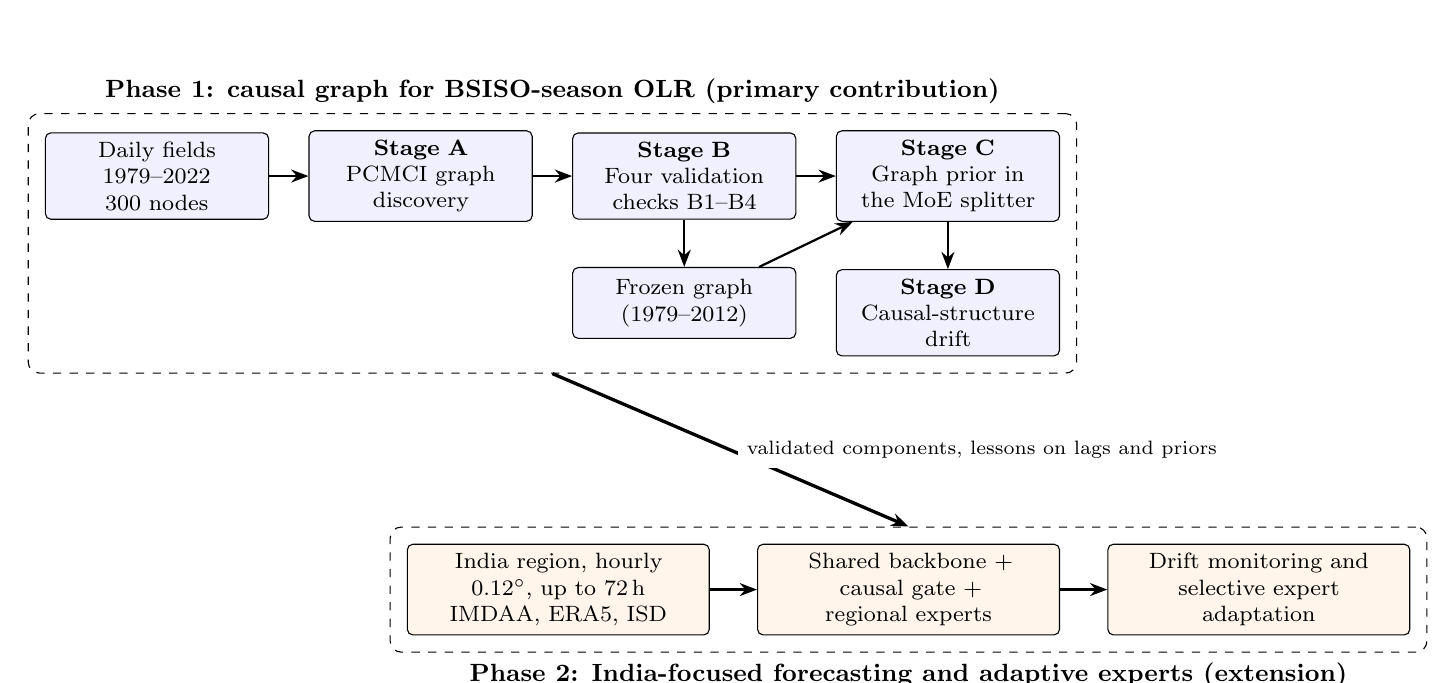
\begin{tikzpicture}[node distance=0.45cm and 0.5cm]
\node[box, fill=blue!6] (data) {Daily fields\\1979--2022\\300 nodes};
\node[box, fill=blue!6, right=of data] (A) {\textbf{Stage A}\\PCMCI graph\\discovery};
\node[box, fill=blue!6, right=of A] (B) {\textbf{Stage B}\\Four validation\\checks B1--B4};
\node[box, fill=blue!6, right=of B] (C) {\textbf{Stage C}\\Graph prior in\\the MoE splitter};
\node[box, fill=blue!6, below=0.6cm of C] (D) {\textbf{Stage D}\\Causal-structure\\drift};
\node[box, fill=blue!6, below=0.6cm of B] (F) {Frozen graph\\(1979--2012)};
\draw[arr] (data) -- (A); \draw[arr] (A) -- (B); \draw[arr] (B) -- (C);
\draw[arr] (B) -- (F); \draw[arr] (F) -- (C); \draw[arr] (C) -- (D);
\node[grp, fit=(data)(A)(B)(C)(D)(F), label={[font=\small\bfseries]above:Phase 1: causal graph for BSISO-season OLR (primary contribution)}] (p1) {};
\node[wbox, fill=orange!8, below=2.6cm of F, xshift=-1.6cm] (P2a) {India region, hourly\\0.12\dg, up to 72\,h\\IMDAA, ERA5, ISD};
\node[wbox, fill=orange!8, right=0.6cm of P2a] (P2b) {Shared backbone +\\causal gate +\\regional experts};
\node[wbox, fill=orange!8, right=0.6cm of P2b] (P2c) {Drift monitoring and\\selective expert\\adaptation};
\draw[arr] (P2a) -- (P2b); \draw[arr] (P2b) -- (P2c);
\node[grp, fit=(P2a)(P2b)(P2c), label={[font=\small\bfseries]below:Phase 2: India-focused forecasting and adaptive experts (extension)}] (p2) {};
\draw[arr, line width=1.2pt] (p1.south) -- node[lbl, right, xshift=2pt, fill=white]{validated components, lessons on lags and priors} (p2.north);
\end{tikzpicture}%
}
\caption{Two-phase research roadmap. Phase~1 builds, validates, freezes and uses a causal graph for BSISO-season OLR forecasting and measures its stability. Phase~2 transfers the components that pass these tests to an India-focused hourly forecasting system. Global-scale forecasting is treated as future work.}
\label{fig:roadmap}
\end{figure}

\section{Organization of the Thesis}
\label{sec:intro-org}

\begin{itemize}
  \item \textbf{Chapter~\ref{chap:lit}} reviews tropical convection and the BSISO, causal discovery for time series, multiple testing and surrogate methods, Mixture-of-Experts models, machine-learning weather forecasting and drift detection, and identifies the research gaps.
  \item \textbf{Chapter~\ref{chap:data}} formalises the forecasting task and describes the data, regional partition, BSISO season, preprocessing and leakage controls.
  \item \textbf{Chapter~\ref{chap:pcmci}} presents the PCMCI methodology, its statistical tests, FDR correction and computational design.
  \item \textbf{Chapter~\ref{chap:validation}} develops the four validation checks and the graph-guided MoE, including the three modes of using the graph and the control priors.
  \item \textbf{Chapter~\ref{chap:experiments}} describes the implementation, the experimental grid, the metrics and the statistical analysis.
  \item \textbf{Chapter~\ref{chap:results}} reports and discusses the results, organised by research question, together with threats to validity.
  \item \textbf{Chapter~\ref{chap:phase2}} presents the India-focused Phase~2 extension.
  \item \textbf{Chapter~\ref{chap:conclusion}} summarises the findings, assesses each objective and outlines future work.
  \item \textbf{Appendices~A--C} give the notation, derivations, configuration tables, experiment registry, reproducibility instructions and decision log.
\end{itemize}

\chapter{Literature Review and Technical Background}
\label{chap:lit}

\section{Introduction and Review Scope}
\label{sec:lit-scope}

This thesis lies at the intersection of four bodies of work that are rarely combined: the dynamics of tropical intraseasonal convection, causal discovery for multivariate time series, conditional-computation models such as the Mixture of Experts, and data-driven weather forecasting under distribution shift. Each field has its own standards of evidence. Atmospheric dynamics asks whether a relationship is physically possible; causal discovery asks whether it survives conditioning on alternative explanations; machine learning asks whether it improves out-of-sample prediction; and the drift literature asks whether it remains valid over time. The review below is organised around these questions rather than paper by paper. It closes with a comparative table (Table~\ref{tab:lit}) and a statement of the research gaps that the thesis addresses.

\section{Tropical Convection and OLR}
\label{sec:lit-olr}

Deep convection in the tropics is organised on scales from individual cumulonimbus to planetary-scale envelopes. Satellite OLR has been the principal large-scale observable of this organisation since the interpolated NOAA record became available~\cite{liebmann1996description}. The physical basis of OLR as a convection proxy is the dependence of emitted infrared flux on cloud-top temperature: the colder the top, the deeper the cloud. Arkin and Meisner~\cite{arkin1987relationship} established the empirical link between cold-cloud fraction and large-scale convective rainfall, and this link underlies the use of OLR in intraseasonal indices~\cite{wheeler2004allseason,lee2013realtime}.

The convection--moisture relationship gives a second physical constraint relevant to this thesis. Bretherton \emph{et al.}~\cite{bretherton2004relationships} showed that tropical oceanic precipitation rises sharply, approximately exponentially, with column water vapour once it exceeds a threshold. Precipitable water (PW) is therefore both a precursor and a consequence of convection, and its relation with OLR is expected to be strong at short lags within a region. The 850\,hPa zonal wind (u850) captures low-level moisture convergence and the westerly flow beneath active monsoon convection; the 200\,hPa zonal wind (u200) captures upper-level outflow and the large-scale baroclinic structure of the convective envelope; the 850\,hPa geopotential height (h850) captures the low-level pressure and wave response; and SST supplies the slowly varying surface boundary condition. The six Phase~1 variables were chosen because each has a documented role in the life cycle of intraseasonal convection.

\section{BSISO Dynamics and Propagation}
\label{sec:lit-bsiso}

Early observational studies identified northward-moving cloud bands over India with periods of 30--50 days~\cite{yasunari1979cloudiness} and 40--50-day OLR variability in northern summer~\cite{lau1986aspects}. Wang and Xie~\cite{wang1997model} provided a theoretical model in which an equatorial Kelvin--Rossby wave packet, modified by the monsoon mean flow, produces the observed north-west to south-east tilted band and its northward movement. Jiang \emph{et al.}~\cite{jiang2004structures} attributed the northward propagation to vertical wind shear and moisture--convection feedback. Goswami and Ajaya Mohan~\cite{goswami2001intraseasonal} and Annamalai and Slingo~\cite{annamalai2001active} linked these oscillations to the active and break phases of the Indian monsoon.

For monitoring and prediction, Lee \emph{et al.}~\cite{lee2013realtime} defined two indices from a multivariate EOF of OLR and u850 anomalies over 10\dg S--40\dg N, 40\dg--160\dg E in May--October. BSISO1, given by the first two principal components, describes the canonical 30--60-day northward and eastward propagating mode; BSISO2, from the third and fourth components, describes the 10--30-day mode. The first two modes explain about 10\% and 7\% of the filtered variance in their analysis, and the index is constructed without a non-causal band-pass filter by removing the mean of the preceding 120 days, which makes it usable in real time. Kikuchi \emph{et al.}~\cite{kikuchi2012bimodal} proposed a bimodal representation distinguishing the MJO-like winter mode from the BSISO summer mode. Sperber and Annamalai~\cite{sperber2008coupled} documented that coupled models struggle to reproduce BSISO propagation, which motivates statistical and data-driven approaches.

Two facts from this literature shape the methodology. First, the BSISO is seasonal, so a graph estimated over all days of the year mixes summer and winter regimes. Second, its envelope propagates at a few metres per second while equatorial waves embedded in it travel faster, which sets the physical speed scales used in Chapter~\ref{chap:validation}.

\section{Climate Teleconnections and Delayed Dependencies}
\label{sec:lit-teleconnections}

Teleconnections are dependencies between distant regions. Classical theory explains how a localised tropical heat source excites a Kelvin-wave response to its east and a Rossby-wave response to its west~\cite{matsuno1966quasi,gill1980simple}, and how tropical SST anomalies force extratropical wave trains~\cite{trenberth1998progress}. Wheeler and Kiladis~\cite{wheeler1999convectively} and Kiladis \emph{et al.}~\cite{kiladis2009convectively} documented convectively coupled equatorial waves in OLR spectra, with Kelvin waves travelling eastward at roughly 15--20\ms when coupled to convection and faster when dry~\cite{kiladis2009convectively}. These results matter because they establish that legitimate dependencies between regions thousands of kilometres apart can act within one or two days, and that a geographic-distance cutoff would wrongly remove them.

Teleconnections also change over time. Krishna Kumar \emph{et al.}~\cite{kumar1999weakening} reported a weakening of the ENSO--Indian monsoon relationship in the late twentieth century. Any data-driven graph is therefore an estimate for a particular period, and its stability must be tested.

\section{Correlation, Autocorrelation and Conditional Independence}
\label{sec:lit-ci}

Atmospheric statistics has long recognised that autocorrelation reduces the effective number of independent samples and inflates the apparent significance of correlations~\cite{wilks2011statistical,bretherton1999effective,wilks1997resampling}. Runge \emph{et al.}~\cite{runge2014quantifying} made a sharper point for lagged relationships: the lagged cross-correlation between two autocorrelated series is not a reliable estimate of either the strength or the delay of their interaction, because it mixes the coupling with the memory of each series. They proposed measures based on graphical models that condition on the past of both series.

Conditional independence is the formal tool behind this idea. Two variables $X$ and $Y$ are conditionally independent given $Z$, written $X\indep Y\mid Z$, if knowing $X$ adds no information about $Y$ once $Z$ is known. Under the causal Markov and faithfulness assumptions, the conditional-independence relations among variables identify the edges of the underlying causal graph up to an equivalence class~\cite{spirtes2000causation,pearl2009causality}. For time series with only lagged links, time order fixes the edge direction, which removes much of that ambiguity~\cite{runge2018causal}. Granger causality~\cite{granger1969investigating} is the time-series special case in which $X$ "Granger-causes" $Y$ if the past of $X$ improves the prediction of $Y$ beyond the past of $Y$ and other variables; it coincides with conditional dependence on the full past under linear-Gaussian assumptions.

\section{Causal Discovery in Multivariate Time Series}
\label{sec:lit-cd}

Methods for causal discovery in time series fall into four families~\cite{runge2019inferring,runge2023causal,camps2023discovering}.

\paragraph{Granger and regression approaches.} Vector autoregression with significance tests, possibly with lasso regularisation~\cite{tibshirani1996regression}, estimates all lagged coefficients jointly. With 300 nodes and 60 lags there are 18{,}000 regressors per target and the regression is ill-conditioned; regularisation helps but makes the significance of individual links hard to interpret. Neural Granger causality~\cite{tank2022neural} extends the idea to nonlinear models with sparsity penalties.

\paragraph{Constraint-based methods.} The PC algorithm~\cite{spirtes2000causation} removes edges by testing conditional independence with conditioning sets of increasing size. In autocorrelated time series a naive application has low power, because the strong autocorrelation of the source makes conditioning sets large and the test statistic noisy~\cite{runge2019detecting}. PCMCI addresses this; PCMCI$^+$~\cite{runge2020discovering} adds contemporaneous links, and LPCMCI~\cite{gerhardus2020high} relaxes causal sufficiency to allow latent confounders.

\paragraph{Score-based and continuous-optimisation methods.} NOTEARS~\cite{zheng2018dags} recasts DAG learning as continuous optimisation with an acyclicity constraint, and DYNOTEARS~\cite{pamfil2020dynotears} extends it to time series. These methods scale with gradient-based solvers but do not provide link-level significance and are sensitive to variable scaling.

\paragraph{Learned and amortised methods.} Neural relational inference~\cite{kipf2018neural} and amortised causal discovery~\cite{lowe2022amortized} train a network to infer interaction graphs from many examples of a system. They can be fast at inference time but need training data with known graphs, which do not exist for the real atmosphere.

\paragraph{Nonlinear state-space methods.} Convergent cross mapping~\cite{sugihara2012detecting} detects coupling in deterministic dynamical systems, and transfer entropy~\cite{schreiber2000measuring} is an information-theoretic analogue of Granger causality. Both are attractive for nonlinear systems but are expensive and data-hungry at the scale considered here.

For this thesis the decisive requirements are link-level significance with error control, explicit lags, scalability to thousands of candidates per target, and an established record in climate applications. PCMCI is the method that satisfies all four.

\section{PCMCI and Related Methods in Climate Science}
\label{sec:lit-pcmci}

Runge \emph{et al.}~\cite{runge2019detecting} introduced PCMCI and showed in numerical experiments that it achieves higher detection power than PC and lasso-Granger approaches at a controlled false-positive rate, particularly for strongly autocorrelated, high-dimensional systems. Its key idea is to separate a condition-selection step (PC1), which finds a small superset of each variable's parents, from the final momentary conditional-independence (MCI) test, which conditions on the parents of both the target and the lagged source. Conditioning on the source's parents removes the influence of the source's own autocorrelation, which is the main cause of false positives and of poorly calibrated tests in climate data. The method is described in detail in Chapter~\ref{chap:pcmci}.

Applications in climate science have used causal-effect networks built with PCMCI to study drivers of the winter stratospheric polar vortex~\cite{kretschmer2016using}, the tropical and mid-latitude drivers of Indian summer monsoon rainfall~\cite{dicapua2020tropical}, and the time-scale dependence of tropical--extratropical interactions in boreal summer~\cite{dicapua2020dominant}. Nowack \emph{et al.}~\cite{nowack2020causal} used causal networks among sea-level pressure modes as fingerprints to evaluate climate models. Saggioro \emph{et al.}~\cite{saggioro2020reconstructing} extended the approach to regime-dependent graphs. Tibau \emph{et al.}~\cite{tibau2022spatiotemporal} built a stochastic climate model with known teleconnections to benchmark such methods. Earlier, Ebert-Uphoff and Deng~\cite{ebert2012causal} applied constraint-based graphical models to atmospheric indices.

Two features distinguish these studies from the present work. First, most target a small number of indices or a handful of dimension-reduced modes, typically tens of variables, whereas this thesis tests a full pool of 300 regional nodes at 60 lags for every target. Second, they use the graph as an end in itself, for understanding or for model evaluation, and do not test whether it improves a forecasting model under matched controls.

\section{Multiple Testing, Surrogate Tests and Graph Robustness}
\label{sec:lit-robust}

\paragraph{Multiple testing.} When thousands of hypotheses are tested, a per-test threshold of 0.05 guarantees many false positives. Benjamini and Hochberg~\cite{benjamini1995controlling} introduced the false discovery rate (FDR), the expected fraction of false positives among rejections, and a step-up procedure controlling it under independence. Benjamini and Yekutieli~\cite{benjamini2001control} showed that the procedure remains valid under positive regression dependence and provided a conservative version for arbitrary dependence. In climatology, Ventura \emph{et al.}~\cite{ventura2004controlling} and Wilks~\cite{wilks2016stippling} argued that FDR control should replace naive per-gridpoint testing, which routinely overstates field significance.

\paragraph{Surrogate data.} Theiler \emph{et al.}~\cite{theiler1992testing} introduced surrogate data to test a null hypothesis by generating series that share chosen properties of the data but are otherwise random. Phase-randomised surrogates preserve the power spectrum, and hence the autocorrelation function, of a series while destroying any phase relation with other series. Schreiber and Schmitz~\cite{schreiber2000surrogate} and Lancaster \emph{et al.}~\cite{lancaster2018surrogate} reviewed refinements such as amplitude-adjusted and iterated surrogates and emphasised that the validity of any surrogate test depends on whether the preserved properties match the null hypothesis of interest. Block bootstrap methods~\cite{kunsch1989jackknife,efron1993introduction} provide an alternative for autocorrelated data.

\paragraph{Robustness of discovered graphs.} Causal-discovery studies typically report the sensitivity of their graphs to significance levels, lag ranges or test choice~\cite{runge2019inferring}. Using surrogate series as \emph{decoy nodes} inside the candidate pool, so that the discovery algorithm itself must reject them alongside the real candidates, is a less common check. It provides a direct empirical estimate of how often a series with realistic autocorrelation but no real coupling is selected under the full pipeline, including FDR correction. Spatial-scale robustness, testing whether links persist when the same field is aggregated differently, is rarely reported, although aggregation is known to change the dependence structure of climate fields~\cite{bretherton1999effective}.

\section{Physical Constraints and Scientific Priors in Causal Discovery}
\label{sec:lit-physics}

Physical knowledge can enter causal discovery as constraints on admissible links, as priors on link probability, or as a post-hoc plausibility check. Di Capua \emph{et al.}~\cite{dicapua2020tropical} used a "theory-guided" approach in which candidate variables were chosen from prior knowledge of monsoon dynamics. Karpatne \emph{et al.}~\cite{karpatne2017theory} and Reichstein \emph{et al.}~\cite{reichstein2019deep} argued more broadly for combining physical knowledge and data-driven learning in Earth system science. A distinctive question for lagged graphs is whether the implied propagation speed of a link, the distance between source and target divided by the lag, is achievable by any physical process carried by the source variable. This turns wave-speed knowledge from equatorial dynamics~\cite{matsuno1966quasi,wheeler1999convectively,kiladis2009convectively} into a link-level test. The literature reviewed did not use it as a systematic check of a discovered graph; Chapter~\ref{chap:validation} develops it as a diagnostic.

\section{Mixture-of-Experts Architectures and Gating Networks}
\label{sec:lit-moe}

The Mixture of Experts was introduced by Jacobs \emph{et al.}~\cite{jacobs1991adaptive} as a set of expert networks combined by a gating network that assigns input-dependent weights, so that each expert specialises in a region of input space. Jordan and Jacobs~\cite{jordan1994hierarchical} extended it to hierarchies trained with expectation--maximisation. In deep learning, sparsely gated MoE layers~\cite{shazeer2017outrageously}, GShard~\cite{lepikhin2021gshard} and Switch Transformers~\cite{fedus2022switch} route each token to one or a few experts, which decouples parameter count from computation; these works also documented load imbalance and the need for auxiliary balancing losses. For graphs, Graph MoE~\cite{wang2023graph} routes nodes to experts with different aggregation behaviour.

In these architectures the gate is learned purely from data and is judged only by downstream loss. In the present work, the role of the gate is played by a \emph{splitter} that decides which source regions feed each target's expert. Such a splitter can be given external information about which sources are plausible, and the question of whether a causal graph is a good form of that information is the subject of Phase~1.

\section{Invariant Learning and Graph Rationales}
\label{sec:lit-invariance}

Invariant causal prediction~\cite{peters2016causal} rests on the observation that the conditional distribution of a target given its causal parents is invariant across environments, whereas relations with non-causal variables can change. Invariant risk minimisation~\cite{arjovsky2019invariant} and risk extrapolation~\cite{krueger2021out} translate this into training objectives that penalise variation of the risk across environments. Wu \emph{et al.}~\cite{wu2022discovering} adapted the idea to graph neural networks as Discovering Invariant Rationales (DIR): a rationale generator splits each input graph into a causal and a non-causal subgraph, the non-causal parts are exchanged between examples to create interventional environments, and the model is trained to minimise the mean and the variance of the risk across those environments. The splitter used in this thesis adapts DIR from graph classification to spatiotemporal regression (Section~\ref{sec:moe-splitter}).

\section{Graph-Guided Learning and Structured Predictor Selection}
\label{sec:lit-graph}

Graph neural networks~\cite{kipf2017semi,battaglia2018relational} propagate information along a given graph and are widely used for spatiotemporal forecasting, for example in traffic~\cite{li2018diffusion}. When no graph is given, models such as MTGNN~\cite{wu2020connecting} learn an adjacency matrix jointly with the forecaster. Learned adjacencies optimise prediction but are not tested for statistical credibility, and fixed geographic adjacencies are credible but may omit remote influences. Structured sparsity methods such as the lasso~\cite{tibshirani1996regression} select predictors by penalised fitting. A causal graph offers a third option: a sparse, explicitly tested, lag-resolved candidate structure that is fixed before training. Whether it helps is an empirical question, and the answer may depend on how the graph enters the model: as a hard restriction, as an initialisation, or as a soft penalty.

\section{Machine Learning for Weather Forecasting}
\label{sec:lit-mlwp}

Data-driven global weather models have advanced rapidly. WeatherBench~\cite{rasp2020weatherbench} and WeatherBench~2~\cite{rasp2024weatherbench2} provide common evaluation protocols. Keisler~\cite{keisler2022forecasting} showed that a graph neural network can produce competitive multi-day global forecasts; FourCastNet~\cite{pathak2022fourcastnet}, Pangu-Weather~\cite{bi2023accurate} and GraphCast~\cite{lam2023learning} matched or exceeded deterministic operational NWP on many variables and lead times; GenCast~\cite{price2025probabilistic} extended this to probabilistic ensemble forecasting; and ECMWF has deployed a data-driven system, AIFS~\cite{lang2024aifs}. Ben~Bouall\`egue \emph{et al.}~\cite{benbouallegue2024rise} assessed such models in an operational-like setting, and Schultz \emph{et al.}~\cite{schultz2021can} discussed the conditions under which deep learning could replace NWP. Oskarsson \emph{et al.}~\cite{oskarsson2023graph} adapted graph-based neural forecasting to limited-area domains, which is directly relevant to the regional focus of Phase~2.

These models are trained on reanalyses such as ERA5~\cite{hersbach2020era5} and are evaluated mainly at medium range. Their inputs are entire global states, and the dependence between regions is learned implicitly. They neither expose a tested statement of which remote regions drive a given target nor adapt to changes in such dependence. The present work does not compete with them on scale; it studies a complementary question about explicit, validated source selection.

\section{Distribution Shift, Regime Detection and Online Adaptation}
\label{sec:lit-drift}

Machine-learning models assume that training and deployment data share a distribution; when the joint distribution of inputs and targets changes, performance degrades~\cite{quinonero2009dataset}. In the streaming setting this is called concept drift~\cite{gama2014survey,lu2019learning}. Detectors such as CUSUM~\cite{page1954continuous} and ADWIN~\cite{bifet2007learning} monitor an error or statistic stream and signal when its distribution changes. In climatology, Rodionov's sequential t-test analysis of regime shifts (STARS)~\cite{rodionov2004sequential} detects shifts in the mean of a time series as they occur, with prewhitening to handle autocorrelation~\cite{rodionov2006use}.

Adapting to drift raises the problem of catastrophic forgetting~\cite{kirkpatrick2017overcoming}. Progressive networks~\cite{rusu2016progressive} and Expert Gate~\cite{aljundi2017expert} avoid forgetting by adding new modules or experts rather than overwriting old ones, and route inputs to the most relevant expert. For climate forecasting, regimes such as ENSO phases recur, which suggests archiving experts and reactivating them when a familiar regime returns. A detector based on forecast error reacts only after skill has degraded; a detector based on the causal structure itself could in principle react earlier, but only if the estimated structure is stable enough between windows that real changes stand out from sampling noise. That condition is tested in Stage~D.

\section{Related Datasets and Benchmarks}
\label{sec:lit-data}

The interpolated OLR record~\cite{liebmann1996description} and atmospheric reanalyses are the standard sources for BSISO research. ERA5~\cite{hersbach2020era5} provides hourly global fields at about 31\,km from 1940 onward. For India, the IMDAA regional reanalysis~\cite{rani2021imdaa} provides hourly fields at about 12\,km for the satellite era. The NOAA Integrated Surface Database~\cite{smith2011integrated} provides hourly station observations worldwide, including Indian stations. WeatherBench~2~\cite{rasp2024weatherbench2} is the most widely used benchmark for global data-driven models. These datasets are the basis of the Phase~2 design (Chapter~\ref{chap:phase2}).

\section{Comparative Summary of Related Work}
\label{sec:lit-table}

Table~\ref{tab:lit} compares representative works along the dimensions that matter for this thesis: whether the method discovers lagged structure, whether that structure is validated independently, whether it is used in a forecasting model, and whether the method addresses temporal change.

\begin{small}
\renewcommand{\arraystretch}{1.2}
\begin{longtable}{>{\raggedright\arraybackslash}p{3.0cm}>{\raggedright\arraybackslash}p{3.3cm}>{\centering\arraybackslash}p{1.15cm}>{\centering\arraybackslash}p{1.15cm}>{\centering\arraybackslash}p{1.15cm}>{\centering\arraybackslash}p{1.15cm}>{\raggedright\arraybackslash}p{2.9cm}}
\caption{Comparison of related work. Columns: \textbf{Lag} = discovers explicit lagged dependencies; \textbf{Val.} = validates the discovered structure with an independent check; \textbf{Fcst.} = uses the structure in a forecasting model; \textbf{Drift} = addresses temporal change. \checkmark\ = yes; $\circ$ = partly; -- = no.}\label{tab:lit}\\
\toprule
\textbf{Work} & \textbf{Approach} & \textbf{Lag} & \textbf{Val.} & \textbf{Fcst.} & \textbf{Drift} & \textbf{Relevance / gap} \\
\midrule
\endfirsthead
\toprule
\textbf{Work} & \textbf{Approach} & \textbf{Lag} & \textbf{Val.} & \textbf{Fcst.} & \textbf{Drift} & \textbf{Relevance / gap} \\
\midrule
\endhead
\bottomrule
\endfoot
Granger~\cite{granger1969investigating} & Predictive causality via regression & \checkmark & -- & $\circ$ & -- & Foundational; no control for common drivers beyond included variables \\
Runge et al.~\cite{runge2014quantifying} & Graph-based coupling measures & \checkmark & -- & -- & -- & Shows lagged correlation is ambiguous in climate data \\
Runge et al.~\cite{runge2019detecting} & PCMCI & \checkmark & $\circ$ & -- & -- & Core method; validated on synthetic systems \\
Runge~\cite{runge2020discovering} & PCMCI$^+$ & \checkmark & $\circ$ & -- & -- & Adds lag-0 links; not needed for forecasting \\
Gerhardus \& Runge~\cite{gerhardus2020high} & LPCMCI & \checkmark & $\circ$ & -- & -- & Handles latent confounders; higher cost \\
Kretschmer et al.~\cite{kretschmer2016using} & Causal effect networks & \checkmark & $\circ$ & $\circ$ & -- & Climate drivers from a few indices \\
Di Capua et al.~\cite{dicapua2020tropical} & Theory-guided CEN, monsoon & \checkmark & $\circ$ & -- & -- & Monsoon drivers; small variable set \\
Saggioro et al.~\cite{saggioro2020reconstructing} & Regime-dependent PCMCI & \checkmark & $\circ$ & -- & \checkmark & Regime-specific graphs; known regimes \\
Nowack et al.~\cite{nowack2020causal} & Causal fingerprints & \checkmark & $\circ$ & -- & -- & Uses graphs to evaluate models \\
Tank et al.~\cite{tank2022neural} & Neural Granger & \checkmark & -- & $\circ$ & -- & Nonlinear; no link-level error control \\
Pamfil et al.~\cite{pamfil2020dynotears} & DYNOTEARS & \checkmark & -- & -- & -- & Scalable; no significance testing \\
Kipf et al.~\cite{kipf2018neural} & NRI & $\circ$ & -- & \checkmark & -- & Learned interactions; needs graph-labelled data \\
Wu et al.~\cite{wu2022discovering} & DIR-GNN rationales & -- & $\circ$ & -- & -- & Invariance-trained selection; adapted here \\
Shazeer et al.~\cite{shazeer2017outrageously} & Sparse MoE & -- & -- & \checkmark & -- & Data-learned gating only \\
Wang et al.~\cite{wang2023graph} & Graph MoE & -- & -- & \checkmark & -- & Experts on graphs; no causal prior \\
Wu et al.~\cite{wu2020connecting} & MTGNN learned graph & $\circ$ & -- & \checkmark & -- & Learned adjacency not tested for credibility \\
Lam et al.~\cite{lam2023learning} & GraphCast & -- & -- & \checkmark & -- & Global ML NWP; implicit dependence \\
Price et al.~\cite{price2025probabilistic} & GenCast & -- & -- & \checkmark & -- & Probabilistic ML NWP \\
Oskarsson et al.~\cite{oskarsson2023graph} & Limited-area graph NWP & -- & -- & \checkmark & -- & Regional ML forecasting \\
Rodionov~\cite{rodionov2004sequential} & STARS & -- & -- & -- & \checkmark & Regime-shift test used in Stage~D \\
Bifet \& Gavald\`a~\cite{bifet2007learning} & ADWIN & -- & -- & $\circ$ & \checkmark & Error-stream drift detection \\
Aljundi et al.~\cite{aljundi2017expert} & Expert Gate & -- & -- & \checkmark & \checkmark & Adding experts without forgetting \\
\midrule
\textbf{This thesis} & PCMCI + four checks + graph prior in MoE + structural drift & \checkmark & \checkmark & \checkmark & \checkmark & Tests credibility and usefulness separately under matched controls \\
\end{longtable}
\end{small}

\section{Research Gaps and Positioning}
\label{sec:lit-gaps}

The comparison identifies four gaps that this thesis addresses.

\begin{enumerate}[label=\textbf{G\arabic*.}]
  \item \textbf{Scale of the candidate pool.} Climate applications of PCMCI typically use tens of pre-selected indices or modes. Running PCMCI over a full pool of 300 regional nodes at 60 lags for every target, without pre-selecting variables by hypothesis, has practical cost and statistical-power implications that have not been documented for intraseasonal OLR.
  \item \textbf{Independent validation of the discovered graph.} Studies report sensitivity to parameters, but a fixed sequence of checks that can each fail, combining decoys inside the discovery pool, a propagation-speed test, data-driven sparsification and persistence across spatial resolution, is not standard practice.
  \item \textbf{Credibility versus usefulness.} Causal graphs in climate science are used for understanding or model evaluation; MoE gates and learned adjacencies in machine learning are judged only by loss. No study among those reviewed tests whether a validated causal graph improves a forecaster's source selection against matched random and correlation priors.
  \item \textbf{Causal structure as a drift signal.} Drift detectors watch error streams, and regime-dependent causal discovery assumes regimes are known. Whether sliding-window changes in an estimated causal structure align with known climate regimes, and could therefore trigger expert adaptation, is an open empirical question.
\end{enumerate}

The thesis is positioned as an applied methodological study. Its novelty lies not in a new discovery algorithm but in the protocol connecting discovery, validation and forecasting use, in the scale at which the protocol is applied, and in reporting the outcome honestly whichever way it falls.

\section{Chapter Summary}
\label{sec:lit-summary}

This chapter reviewed the physical basis of OLR and the BSISO, the reasons why correlation is an unreliable guide to lagged dependence in climate data, the main families of causal-discovery methods and the reasons for choosing PCMCI, the statistical tools for multiple testing and surrogate validation, the Mixture-of-Experts and invariant-learning literature on which the forecasting model builds, recent machine-learning weather models, and drift detection. It identified four gaps. The next chapter formalises the forecasting problem and the data.

\chapter{Problem Formulation, Dataset, and Preprocessing}
\label{chap:data}

\section{Formal Definition of the Forecasting Task}
\label{sec:data-task}

Let $t\in\{1,\dots,T\}$ index days and let $Y^r_t$ denote the standardised OLR anomaly averaged over region $r\in\{0,\dots,R-1\}$ on day $t$, with $R=50$. For a lead time $L$ (in days), the forecasting task is to estimate $Y^r_{t+L}$ from information available at the issue time $t$:
\begin{equation}
  \hat{Y}^{r}_{t+L} = f_{r}\!\left(\{X^{i}_{t-\ell}: i\in\mathcal{N}_r,\;\ell\in\Lambda\}\right),
  \label{eq:task}
\end{equation}
where $X^i_t$ is the standardised anomaly of node $i$ (Section~\ref{sec:data-matrix}), $\mathcal{N}_r$ is the set of nodes available to the forecaster of region $r$, and $\Lambda$ is the set of input lags. The forecast is \emph{direct}: a separate model maps the state at time $t$ to the value at $t+L$, with no autoregressive roll-out. The primary lead is $L=7$ days, which is the horizon of the research question; $L=1$ day is used as a secondary horizon. The question studied in this thesis is how $\mathcal{N}_r$, the set of source regions available to each forecaster, should be chosen, and whether a validated causal graph is a good basis for that choice.

A forecast is \emph{scored} only if its target day $t+L$ lies in the BSISO active season $\Tseason$ (Section~\ref{sec:data-season}) and in the test period $\Ttest=$ 2013--2022. The inputs may come from any earlier day.

\section{Mathematical Representation of the 300-Node System}
\label{sec:data-matrix}

\subsection{Variables}
The six variables are listed in Table~\ref{tab:variables} with their physical interpretation and role in tropical convection. All are provided as daily anomalies on the native grid.

\begin{table}[htbp]
\centering
\caption{The six Phase~1 variables, their typical physical units before anomaly processing, and their role in tropical intraseasonal convection. The data used here are standardised anomalies and are therefore dimensionless.}
\label{tab:variables}
\footnotesize
\renewcommand{\arraystretch}{1.25}
\begin{tabularx}{\textwidth}{>{\raggedright\arraybackslash}p{1.25cm}>{\raggedright\arraybackslash}p{2.6cm}>{\raggedright\arraybackslash}p{1.45cm}>{\raggedright\arraybackslash}X>{\raggedright\arraybackslash}p{2.6cm}}
\toprule
\textbf{Symbol} & \textbf{Variable} & \textbf{Units} & \textbf{Physical role} & \textbf{Typical time scale} \\
\midrule
SST & Sea surface temperature & K & Surface boundary condition; modulates surface heat and moisture fluxes that sustain convection; responds to cloud shading and wind-driven evaporation & Weeks to months (slow) \\
h850 & Geopotential height at 850\,hPa & m (geopotential metres) & Low-level pressure field; marks the Rossby- and Kelvin-wave response to convective heating and monsoon troughs & Days to weeks \\
u200 & Zonal wind at 200\,hPa & m\,s$^{-1}$ & Upper-tropospheric outflow above convection; large-scale overturning circulation & Days to weeks \\
PW & Precipitable water & kg\,m$^{-2}$ (mm) & Column moisture; strong precursor of deep convection above a critical value~\cite{bretherton2004relationships} & Days \\
u850 & Zonal wind at 850\,hPa & m\,s$^{-1}$ & Low-level monsoon westerlies and moisture convergence; one of the two BSISO index fields~\cite{lee2013realtime} & Days to weeks \\
OLR & Outgoing longwave radiation & W\,m$^{-2}$ & Convection proxy: low OLR indicates cold, high cloud tops~\cite{arkin1987relationship}; the forecast target & Days (fast) \\
\bottomrule
\end{tabularx}
\end{table}

\subsection{Nodes and the state matrix}
A node $i=(r,v)$ is a variable $v\in\mathcal{V}$ averaged over a region $r$. With $R=50$ regions and $|\mathcal{V}|=6$ variables there are
\begin{equation}
  N = R\,|\mathcal{V}| = 50\times 6 = 300
\end{equation}
nodes. Let $\Omega_r$ be the set of grid cells assigned to region $r$ and $\Omega^{\mathrm{ocean}}_r\subseteq\Omega_r$ its ocean cells. The raw regional series is
\begin{equation}
  Z^{(r,v)}_t = \frac{1}{|\Omega^{v}_r|}\sum_{c\in\Omega^{v}_r} A^{v}_{c,t},
  \qquad
  \Omega^{v}_r = \begin{cases}\Omega^{\mathrm{ocean}}_r & v=\mathrm{SST},\\ \Omega_r & \text{otherwise},\end{cases}
  \label{eq:regionmean}
\end{equation}
where $A^v_{c,t}$ is the gridded anomaly of variable $v$ in cell $c$ on day $t$. SST is averaged only over ocean cells because it is undefined over land. Each node is then re-standardised with statistics computed only on the development period:
\begin{equation}
  X^{i}_t = \frac{Z^{i}_t - \mu_i}{\sigma_i},\qquad
  \mu_i = \frac{1}{|\Ttrain|}\sum_{t\in\Ttrain} Z^i_t,\quad
  \sigma_i^2 = \frac{1}{|\Ttrain|}\sum_{t\in\Ttrain}(Z^i_t-\mu_i)^2 .
  \label{eq:standardise}
\end{equation}
The system state on day $t$ is $\mathbf{X}_t=(X^{1}_t,\dots,X^{N}_t)^{\top}\in\R^{N}$, and the full data form the matrix $\mathbf{X}\in\R^{T\times N}$ with $T=16{,}071$ days. Figure~\ref{fig:nodes} shows the structure.

Region means in Eq.~\eqref{eq:regionmean} are unweighted averages of the member cells. On a 2.5\dg\ grid within 30\dg\ of the equator, the cell area varies by at most a factor of $\cos 30\dg\approx 0.87$, so area weighting would change the means only slightly; it is recorded as an implementation choice in Appendix~\ref{app:decisions}.

\begin{figure}[htbp]
\centering
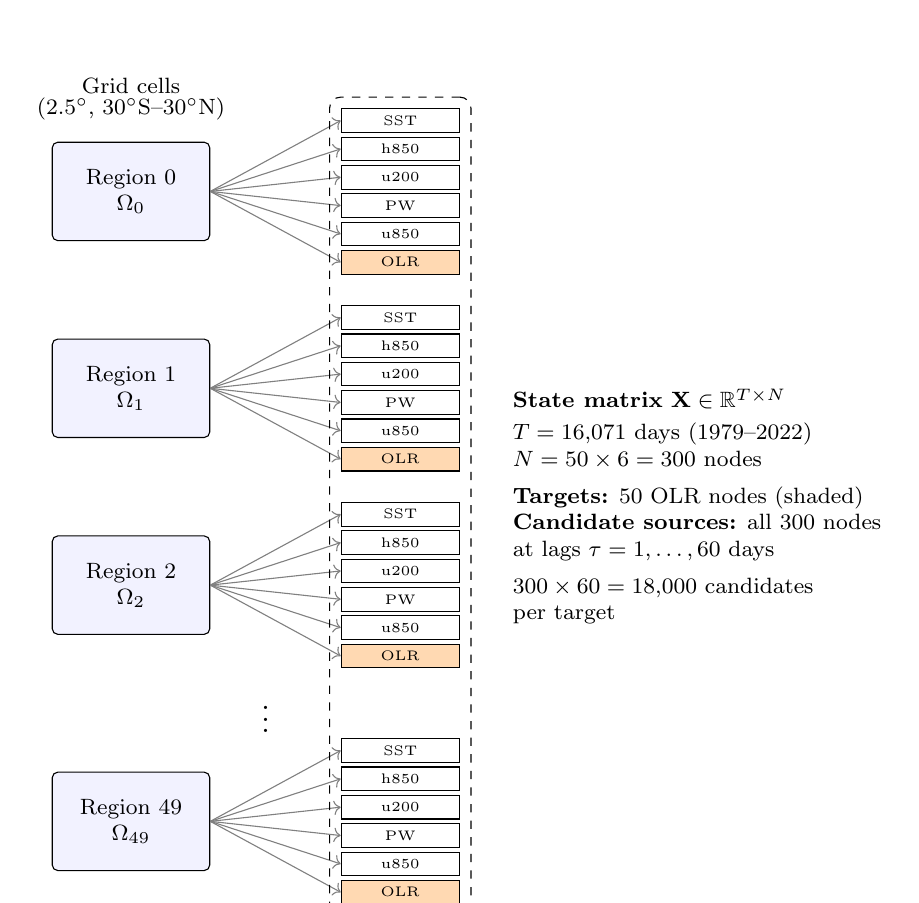
\begin{tikzpicture}[x=0.95cm,y=1cm]
% region blocks
\foreach \r/\lab/\yy in {0/0/0, 1/1/-2.5, 2/2/-5.0, 3/49/-8.0}{
  \node[draw, rounded corners=2pt, minimum width=2.0cm, minimum height=1.25cm, fill=blue!5, font=\footnotesize, align=center] (R\r) at (0,\yy) {Region \lab\\$\Omega_{\lab}$};
  \foreach \v/\nm [count=\k from 0] in {SST,h850,u200,PW,u850,OLR}{
    \pgfmathsetmacro{\py}{\yy+0.9-0.36*\k}
    \ifnum\k=5
      \node[draw, fill=orange!30, minimum width=1.5cm, minimum height=0.3cm, font=\tiny, inner sep=1pt] (n\r\k) at (3.6,\py) {\nm};
    \else
      \node[draw, fill=white, minimum width=1.5cm, minimum height=0.3cm, font=\tiny, inner sep=1pt] (n\r\k) at (3.6,\py) {\nm};
    \fi
    \draw[->, gray] (R\r.east) -- (n\r\k.west);
  }
}
\node at (1.8,-6.6) {\large$\vdots$};
\node[draw, dashed, rounded corners, fit=(n00)(n35), inner sep=4pt] (allnodes) {};
\node[font=\footnotesize, align=left, right=0.4cm of allnodes] (mat) {%
  \textbf{State matrix} $\mathbf{X}\in\mathbb{R}^{T\times N}$\\[2pt]
  $T=16{,}071$ days (1979--2022)\\
  $N=50\times 6=300$ nodes\\[4pt]
  \textbf{Targets:} 50 OLR nodes (shaded)\\
  \textbf{Candidate sources:} all 300 nodes\\
  at lags $\tau=1,\dots,60$ days\\[4pt]
  $300\times 60=18{,}000$ candidates\\ per target};
\node[font=\footnotesize, align=center, above=0.15cm of R0] {Grid cells\\[-2pt](2.5\dg, 30\dg S--30\dg N)};
\end{tikzpicture}
\caption{Schematic of the 300-node representation. Each of the 50 regions contributes six regional-mean variables. The 50 OLR nodes (shaded) are the forecast targets; all 300 nodes are candidate sources at lags of 1--60 days. The diagram is schematic and does not show the real region geometry.}
\label{fig:nodes}
\end{figure}

\subsection{Candidate source--target--lag combinations}
\label{sec:data-candidates}
For one OLR target node $j$, every node $i\in\{1,\dots,300\}$, including $j$ itself, is a candidate source at every lag $\tau\in\{1,\dots,60\}$, which gives
\begin{equation}
  |\mathcal{C}_j| = N\,\taumax = 300\times 60 = 18{,}000
\end{equation}
lagged candidates per target and $50\times 18{,}000 = 900{,}000$ for the 50 OLR targets. If instead every ordered pair of \emph{distinct} nodes were considered with all 300 nodes as targets, the count would be
\begin{equation}
  N(N-1)\,\taumax = 300\times 299\times 60 = 5{,}382{,}000 .
\end{equation}
These numbers count candidate hypotheses before screening, not statistical tests performed: PCMCI's screening stage (Chapter~\ref{chap:pcmci}) removes most candidates after few tests, and the final MCI test is applied only to the survivors. They nonetheless explain why FDR control and an efficient implementation are essential.

\section{Regional Partition}
\label{sec:data-regions}

The native grid has $25\times 144=3{,}600$ cells. Individual cells are noisy and too numerous for a 60-lag analysis, and a single 2.5\dg\ cell has no physical significance. The cells are therefore grouped into 50 regions by $k$-means clustering~\cite{lloyd1982least} applied to the cells' OLR time series over the development period, so that cells whose convection varies together form a region. In practice 46 of the 50 regions are single contiguous areas, and each region contains on average 72 cells. A region adjacency graph is derived from whether any two cells of different regions touch, with longitude wrapping around the date line. The regions are indexed 0--49; this numbering is used in all result figures.

For the resolution check (Section~\ref{sec:val-b4}), each region is split into two sub-regions by $k$-means with $k=2$ applied to its own cells, giving 100 nested regions. Because some sub-regions contain no ocean cells, the 100-region representation has 596 rather than 600 nodes.

Clustering on OLR co-variability and then searching for OLR dependencies between the clusters introduces a mild circularity: regions are, by construction, internally coherent in OLR, and the boundaries between them fall where OLR co-variability drops. The effect is to make between-region OLR links harder rather than easier to detect, but it does mean that the regions are not independent of the target variable. The point is revisited in the threats to validity (Section~\ref{sec:res-validity}). Geographic adjacency, used to define local candidate pools for the forecaster (Section~\ref{sec:moe-pools}), is a separate rule based only on geometry.

\section{Temporal Coverage and Data Provenance}
\label{sec:data-provenance}

Table~\ref{tab:provenance} summarises the data. The fields come from a BSISO monitoring archive in which each variable is stored as a daily anomaly on a common 2.5\dg\ grid covering 30\dg S--30\dg N and all longitudes, from 1 January 1979 to 31 December 2022. The record has 16{,}071 days with no missing days. Each field was anomaly-processed upstream: a daily climatology was removed and the anomalies were normalised separately at each grid cell. A land--sea mask identifies ocean cells for SST.

\begin{table}[htbp]
\centering
\caption{Phase~1 data summary. Items marked [confirm] must be checked against the original archive documentation before submission.}
\label{tab:provenance}
\footnotesize
\renewcommand{\arraystretch}{1.2}
\begin{tabularx}{\textwidth}{>{\raggedright\arraybackslash}p{4.0cm}>{\raggedright\arraybackslash}X}
\toprule
\textbf{Property} & \textbf{Value} \\
\midrule
Archive & Pre-processed BSISO monitoring fields (\texttt{rt\_preprocessed\_archive}); originating reanalysis and OLR products [confirm] \\
Variables & SST, h850, u200, PW, u850, OLR \\
Grid & $2.5\dg\times 2.5\dg$; 25 latitudes (30\dg N to 30\dg S) $\times$ 144 longitudes (0\dg--357.5\dg E) \\
Period & 1979-01-01 to 2022-12-31; 16{,}071 daily values; no missing days \\
Pre-processing upstream & Daily climatology removed and anomalies normalised per grid cell; climatology base period 1979--2014 \\
Auxiliary data & Ocean mask ($25\times 144$, Boolean) \\
Licence & [confirm with archive provider] \\
Development / test split & 1979--2012 / 2013--2022 \\
\bottomrule
\end{tabularx}
\end{table}

\section{Target Construction and Forecast Lead Time}
\label{sec:data-target}

The target of region $r$ at lead $L$ is $Y^{r}_{t+L}=X^{(r,\mathrm{OLR})}_{t+L}$. Two leads are studied:
\begin{itemize}
  \item $L=7$ days, the primary horizon of the research question, at which OLR retains almost no persistence;
  \item $L=1$ day, a secondary horizon at which persistence is very strong and the graph's short-lag links act on the same time scale as the forecast.
\end{itemize}
The input to the forecaster of region $r$ is built from source regions $r'\in\mathcal{C}_r$. For each source region, the six variables are taken at the seven input lags $\Lambda=\{0,1,2,3,5,7,10\}$ days before the issue time, and an ocean-fraction feature is appended, giving a 49-dimensional vector
\begin{equation}
  \mathbf{h}^{r'}_t = \big[\,X^{(r',v)}_{t-\ell}\;:\;v\in\mathcal{V},\;\ell\in\Lambda\,\big]\;\|\;\phi_{r'}\;\in\R^{49},
  \label{eq:features}
\end{equation}
where $\phi_{r'}$ is the ocean fraction of region $r'$ and $\|$ denotes concatenation. The irregular lag set gives dense coverage of the most recent days and sparser coverage further back. The splitter additionally sees a window of the last 10 days of each region's state.

\section{BSISO Season and Activity-Based Target Selection}
\label{sec:data-season}

\subsection{Why an activity-based season}
A fixed calendar window such as May--October treats a year with an early and vigorous BSISO in the same way as a year in which the oscillation is weak until July. Because the graph is meant to describe dependencies that operate when the BSISO is active, the season is defined by the oscillation's own amplitude, with a margin so that onset and decay are included.

\subsection{Reproducing the BSISO index}
The index follows the BSISO1 recipe of Lee \emph{et al.}~\cite{lee2013realtime}, adapted to the available grid:
\begin{enumerate}
  \item OLR and u850 anomalies are taken over 10\dg S--30\dg N, 40\dg--160\dg E. Lee \emph{et al.} use 10\dg S--40\dg N; the data stop at 30\dg N.
  \item The mean of the preceding 120 days is subtracted at each grid point to isolate intraseasonal variability without a non-causal band-pass filter.
  \item Each grid point is weighted by $\sqrt{\cos\varphi}$, where $\varphi$ is latitude, and each field is divided by its domain-mean standard deviation so that OLR and u850 contribute equally.
  \item A combined EOF~\cite{hannachi2007empirical,north1982sampling} is computed on May--October days of the development years only (1979--2012), so that test years never influence the patterns.
  \item The first two principal components are normalised to unit variance over the fit days, and the BSISO amplitude is
  \begin{equation}
    A_t = \sqrt{\mathrm{PC1}_t^2 + \mathrm{PC2}_t^2}.
    \label{eq:amp}
  \end{equation}
\end{enumerate}

\subsection{Season definition}
For each year, the 31-day centred running mean $\bar{A}_t$ of the amplitude is computed inside a search window from 1 April to 30 November. The season starts at the first day of the first run of at least 20 consecutive days with $\bar{A}_t>1$, ends at the last day of the last such run, and is padded by 21 days on each side:
\begin{equation}
  \Tseason_y = \big[\,t^{\mathrm{on}}_y - 21,\; t^{\mathrm{off}}_y + 21\,\big].
  \label{eq:season}
\end{equation}
A year with no qualifying run falls back to 1 May--31 October. The resulting season averages 208 days per year, ranges from 82 to 286 days, and begins between April and July. The development years contain 7{,}153 season days. Figure~\ref{fig:season} in Chapter~\ref{chap:results} shows the amplitude climatology and the season of each year.

The 31-day running mean is centred and therefore uses up to 15 days after a given day. This is acceptable because the season mask decides only \emph{which} target days are scored; it is never an input to a forecast. The consequence is that evaluation is conditioned on the BSISO having been active, which is the intended scope.

\subsection{Target days versus source history}
The season restricts target days only. A source value at lag $\tau$ is read from day $t-\tau$ regardless of whether that day is in the season. For a target on 1 June, a lag-45 source value comes from mid-April. Removing all non-season days before building the lags would delete exactly the precursor information that the analysis is meant to find, and would create artificial discontinuities at the season boundaries. Formally, the PCMCI sample for target node $j$ is
\begin{equation}
  \mathcal{D}_j = \big\{\,(X^j_t,\;\{X^{i}_{t-\tau}\}_{i,\tau})\;:\; t\in\Tseason\cap\Ttrain,\; t-2\taumax\ge 1\,\big\},
  \label{eq:sample}
\end{equation}
where the requirement $t-2\taumax\ge 1$ ensures that the lagged conditioning values of the MCI test (Section~\ref{sec:pcmci-mci}) lie inside the record.

\section{Climatology, Anomalies, Standardisation and Units}
\label{sec:data-anomalies}

\subsection{Why the seasonal cycle must be removed}
Almost every climate variable has a strong annual cycle. Two unrelated series that both peak in boreal summer are strongly correlated at every lag shorter than a few months, purely because of their shared calendar dependence. If the annual cycle were left in the data, PCMCI would find dense, spurious lagged links driven by the calendar, and the forecaster would learn the seasonal cycle rather than intraseasonal dynamics. The standard remedy is to subtract a smoothed daily climatology,
\begin{equation}
  A^{v}_{c,t} = V^{v}_{c,t} - \bar{V}^{v}_{c}\big(d(t)\big),
  \qquad
  \bar{V}^{v}_{c}(d) = \sum_{h=0}^{H} \big[a_{h}\cos(2\pi h d/365.25) + b_{h}\sin(2\pi h d/365.25)\big],
  \label{eq:clim}
\end{equation}
where $V^{v}_{c,t}$ is the raw field, $d(t)$ is the day of year and $\bar{V}$ is a smoothed climatology, here written as the common choice of the mean and first $H$ annual harmonics. The anomalies are then standardised.

\subsection{Implementation in this work}
The fields arrive as anomalies with respect to an upstream daily climatology computed over 1979--2014 and normalised per grid cell. The exact smoothing rule and leap-day treatment of the upstream climatology are those of the archive [confirm]. This work adds two steps: (i) the regional means of Eq.~\eqref{eq:regionmean} are re-standardised with development-period statistics only (Eq.~\eqref{eq:standardise}); and (ii) the BSISO index removes the preceding 120-day mean before the EOF analysis.

The upstream base period overlaps the test period by two years (2013 and 2014). A climatology contains, for each calendar day, an average over 36 years; two of those years being test years means that roughly $2/36\approx 6\%$ of the information in the climatology comes from the test period. The effect on forecast scores is expected to be small, because the climatology is a smooth function of calendar day and all models compared in this thesis share it, but it is a genuine departure from a fully clean split and is listed as a limitation (Section~\ref{sec:res-validity}). Refitting the climatology on 1979--2012 requires reprocessing the gridded archive and is included in future work.

\section{Missing Data and Quality Control}
\label{sec:data-qc}

The archive contains no missing days. Quality control at the regional level consists of (i) checking that every region has at least one ocean cell for SST, which holds at 50 regions but not for 4 of the 100 sub-regions, whose SST nodes are dropped; (ii) checking that each node has a non-zero development-period variance before standardisation; and (iii) confirming that the season mask produces a non-empty season every year. Because there are no gaps, no imputation is performed. A future multi-source dataset (Phase~2) will need an explicit gap and outlier policy.

\section{Lag Construction and Temporal Alignment}
\label{sec:data-lags}

All series share a common daily time axis. For a target day $t$, the candidate value of node $i$ at lag $\tau$ is $X^{i}_{t-\tau}$. Lag $0$ is excluded from graph discovery: a link must point from the past to the present, so its direction follows from time order, and contemporaneous dependence, which cannot be oriented without further assumptions~\cite{runge2020discovering}, is outside scope. For forecasting at lead $L$, the newest usable value of any source is at the issue time $t$, so a source that is a parent of $Y_{t+L}$ at lag $\tau$ can be used directly only if $\tau\ge L$. This forecast-time availability condition is central to interpreting the Stage~C results and is discussed in Section~\ref{sec:moe-availability}.

\section{Development and Holdout Split}
\label{sec:data-split}

\begin{figure}[htbp]
\centering
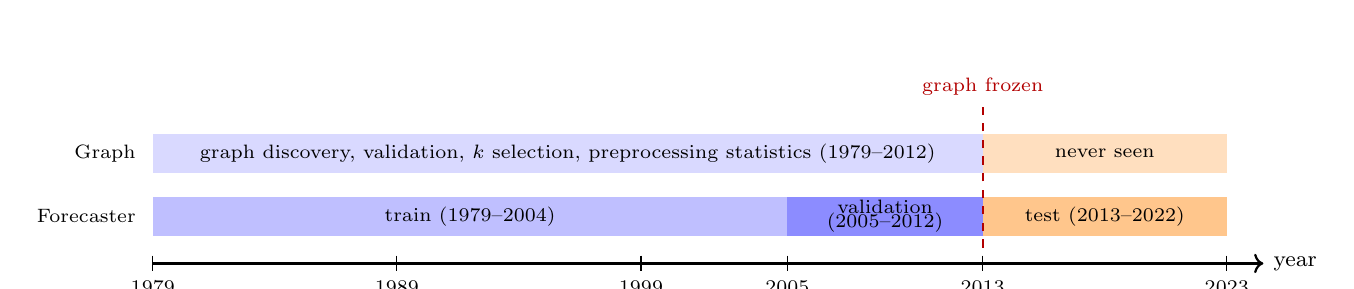
\begin{tikzpicture}[x=0.31cm,y=1cm]
\draw[thick,->] (0,0) -- (45.5,0) node[right,font=\footnotesize]{year};
\foreach \y/\lab in {0/1979, 10/1989, 20/1999, 26/2005, 34/2013, 44/2023}{
  \draw (\y,0.1) -- (\y,-0.1) node[below,font=\scriptsize]{\lab};
}
\fill[blue!25] (0,0.35) rectangle (26,0.85);
\node[font=\scriptsize] at (13,0.6) {train (1979--2004)};
\fill[blue!45] (26,0.35) rectangle (34,0.85);
\node[font=\scriptsize, align=center] at (30,0.6) {validation\\[-3pt](2005--2012)};
\fill[orange!45] (34,0.35) rectangle (44,0.85);
\node[font=\scriptsize] at (39,0.6) {test (2013--2022)};
\fill[blue!15] (0,1.15) rectangle (34,1.65);
\node[font=\scriptsize] at (17,1.4) {graph discovery, validation, $k$ selection, preprocessing statistics (1979--2012)};
\fill[orange!25] (34,1.15) rectangle (44,1.65);
\node[font=\scriptsize] at (39,1.4) {never seen};
\node[font=\scriptsize, anchor=east] at (-0.3,1.4) {Graph};
\node[font=\scriptsize, anchor=east] at (-0.3,0.6) {Forecaster};
\draw[dashed, thick, red!70!black] (34,0.2) -- (34,2.0) node[above,font=\scriptsize]{graph frozen};
\end{tikzpicture}
\caption{Phase~1 time split. Everything that shapes the graph or the forecaster, including the preprocessing statistics, the BSISO EOF patterns, PCMCI, the validation checks and the choice of $k$, uses 1979--2012 only. The graph is frozen before 2013--2022 is used, and test years are used only for scoring.}
\label{fig:timeline}
\end{figure}

Figure~\ref{fig:timeline} shows the split. The development period $\Ttrain$ (1979--2012) is used for graph discovery and for training. Within it, the forecaster uses 1979--2004 for fitting and 2005--2012 for validation, and the top-$k$ check fits on 1979--2004 and scores on 2005--2012 season days. The test period $\Ttest$ (2013--2022) is held out: it provides 1{,}989 season target days for evaluation. A chronological split rather than random cross-validation is used because random folds of autocorrelated series place nearly identical days in training and test sets and overstate skill~\cite{bergmeir2012use}.

\section{Leakage Prevention}
\label{sec:data-leakage}

Leakage occurs when information that would not be available at prediction time influences model construction~\cite{kaufman2012leakage}. Table~\ref{tab:leakage} lists each possible channel and the control applied.

\begin{table}[htbp]
\centering
\caption{Leakage channels and controls in Phase~1.}
\label{tab:leakage}
\footnotesize
\renewcommand{\arraystretch}{1.2}
\begin{tabularx}{\textwidth}{>{\raggedright\arraybackslash}p{4.0cm}>{\raggedright\arraybackslash}X}
\toprule
\textbf{Channel} & \textbf{Control} \\
\midrule
Node standardisation & Means and variances from 1979--2012 only (Eq.~\eqref{eq:standardise}) \\
Regional partition & $k$-means fitted on the development span \\
BSISO EOF patterns & Fitted on May--October days of 1979--2012 only \\
Graph discovery and validation & PCMCI, decoys, lag mask, persistence on 1979--2012 season days only \\
Choice of $k$ & Fit 1979--2004, score 2005--2012 \\
Correlation-prior ranking & Lagged correlations computed on training rows only \\
Forecaster training and early choices & 1979--2004 train, 2005--2012 validation \\
Climatology baseline & Mean of the training targets \\
Upstream anomaly climatology & Base period 1979--2014; two-year overlap acknowledged as a limitation \\
Season mask & Selects scored days only; never an input to a forecast \\
\bottomrule
\end{tabularx}
\end{table}

\section{Unresolved Dataset Decisions}
\label{sec:data-open}

Three dataset decisions remain open and are recorded in the decision log (Appendix~\ref{app:decisions}): (i) confirmation of the originating products and licence of the archive; (ii) refitting of the anomaly climatology on 1979--2012 to remove the overlap with the test years; and (iii) the use of a second, independent reanalysis or OLR product to test whether the graph depends on the data source. None of them affects the internal consistency of the comparisons in this thesis, because every model is evaluated on identical inputs and targets.

\section{Chapter Summary}
\label{sec:data-summary}

This chapter defined the direct seven-day OLR forecasting task, the 300-node representation built from 50 OLR-coherent regions and six variables, the 49-dimensional regional feature vectors, the activity-based BSISO season reproduced from the project's own data, and the development/test split with its leakage controls. The next chapter describes how PCMCI turns the 18{,}000 candidates per target into a sparse lagged graph.

\chapter{Proposed Methodology: PCMCI and Graph Discovery}
\label{chap:pcmci}

\section{Overview of the Causal-Discovery Pipeline}
\label{sec:pcmci-overview}

Stage~A turns the 300-node state matrix into a lagged graph whose edges point into the 50 OLR targets. Figure~\ref{fig:pcmci-pipeline} shows the sequence. For each target, a lagged design matrix is built from the season target days of the development period; the PC1 stage screens the 18{,}000 candidates down to a small superset of parents; the MCI stage retests each survivor while conditioning on the parents of both the target and the source; and the Benjamini--Hochberg procedure controls the false discovery rate over all candidates of that target. The output is a list of links, each with a source node, a lag, a signed strength and an adjusted $q$-value.

\begin{figure}[htbp]
\centering
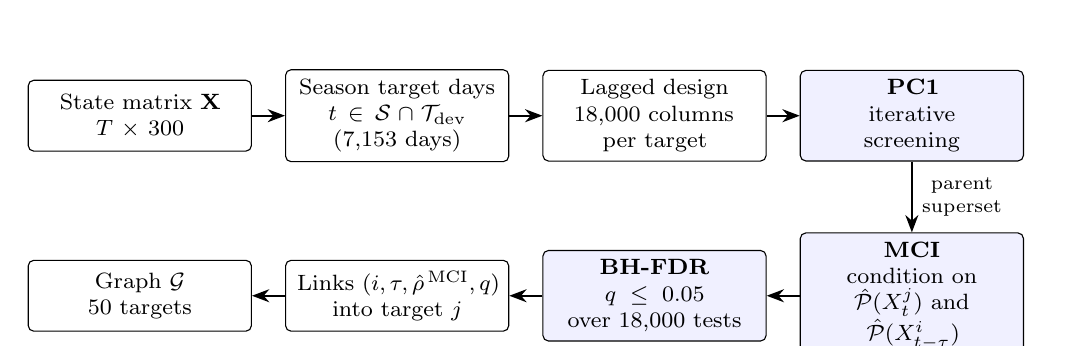
\begin{tikzpicture}[node distance=0.35cm and 0.42cm]
\node[box] (X) {State matrix $\mathbf{X}$\\$T\times 300$};
\node[box, right=of X] (S) {Season target days\\$t\in\Tseason\cap\Ttrain$\\(7{,}153 days)};
\node[box, right=of S] (D) {Lagged design\\18{,}000 columns\\per target};
\node[box, right=of D, fill=blue!6] (PC) {\textbf{PC1}\\iterative\\screening};
\node[box, below=0.9cm of PC, fill=blue!6] (MCI) {\textbf{MCI}\\condition on\\$\hat\Pa(X^j_t)$ and $\hat\Pa(X^i_{t-\tau})$};
\node[box, left=of MCI, fill=blue!6] (FDR) {\textbf{BH-FDR}\\$q\le 0.05$\\over 18{,}000 tests};
\node[box, left=of FDR] (G) {Links $(i,\tau,\MCI,q)$\\into target $j$};
\node[box, left=of G] (Gall) {Graph $\mathcal{G}$\\50 targets};
\draw[arr] (X) -- (S); \draw[arr] (S) -- (D); \draw[arr] (D) -- (PC);
\draw[arr] (PC) -- node[lbl,right]{parent\\superset} (MCI);
\draw[arr] (MCI) -- (FDR); \draw[arr] (FDR) -- (G); \draw[arr] (G) -- (Gall);
\node[lbl, below=0.1cm of PC.south east, anchor=north west] {};
\end{tikzpicture}
\caption{Stage~A pipeline. For each OLR target node $j$, PC1 screens 18{,}000 lagged candidates down to a parent superset; MCI retests every survivor conditioned on the parents of both target and source; Benjamini--Hochberg correction controls the FDR over all candidates of the target. Only development-period season days are used.}
\label{fig:pcmci-pipeline}
\end{figure}

\section{Graph Notation and Node Definitions}
\label{sec:pcmci-notation}

We assume that the standardised node series follow a lagged structural model
\begin{equation}
  X^{j}_t = g_j\!\left(\Pa(X^j_t),\,\eta^j_t\right),\qquad j=1,\dots,N,
  \label{eq:scm}
\end{equation}
where $\Pa(X^j_t)\subseteq\{X^{i}_{t-\tau}: i=1,\dots,N;\;\tau=1,\dots,\taumax\}$ is the set of lagged parents of $X^j_t$, $g_j$ is a function, and the noise terms $\eta^j_t$ are mutually independent and independent of the past. The associated time-series graph $\mathcal{G}$ has a node for every pair $(i,t)$ and a directed edge $X^i_{t-\tau}\to X^j_t$ whenever $X^i_{t-\tau}\in\Pa(X^j_t)$. Under stationarity the edge set is the same for every $t$, so $\mathcal{G}$ is summarised by the set of lagged links
\begin{equation}
  \mathcal{E}=\big\{(i,j,\tau): X^{i}_{t-\tau}\in\Pa(X^j_t)\big\}.
\end{equation}
In this thesis only the parents of the 50 OLR nodes are estimated; the parents of the other 250 nodes are needed only as conditioning sets in the MCI stage.

\section{Conditional-Independence Foundations}
\label{sec:pcmci-ci}

\subsection{Why correlation is insufficient}
Consider three cases in which $X^i_{t-\tau}$ and $X^j_t$ are correlated although $X^i$ has no direct influence on $X^j$:
\begin{itemize}
  \item \textbf{Autocorrelation and indirect paths.} If $X^i_{t-\tau-1}\to X^j_t$ is a true link and $X^i$ is autocorrelated, then $X^i_{t-\tau}$ is also correlated with $X^j_t$. The lagged correlation function of an autocorrelated source is smeared over many lags~\cite{runge2014quantifying}.
  \item \textbf{Common driver.} If $X^k_{t-5}\to X^i_{t-3}$ and $X^k_{t-5}\to X^j_t$, then $X^i_{t-3}$ and $X^j_t$ are correlated at lag 3 without any link between them. In the tropics, an active BSISO phase is such a driver for many regions simultaneously.
  \item \textbf{Mediated path.} If $X^i_{t-2}\to X^m_{t-1}\to X^j_t$, then $X^i_{t-2}$ is correlated with $X^j_t$ but has no direct link to it.
\end{itemize}
In each case the spurious dependence disappears once the right variables are conditioned on: the source's own past in the first case, the common driver in the second, the mediator in the third. Conditional independence is the formal statement of this idea.

\subsection{Conditional independence and its testing}
$X\indep Y\mid\mathbf{Z}$ holds if $p(x\mid y,\mathbf{z})=p(x\mid\mathbf{z})$. Under the causal Markov condition, a variable is independent of its non-descendants given its parents; under faithfulness, every conditional independence in the data is implied by the graph structure~\cite{spirtes2000causation,pearl2009causality}. Together, and assuming causal sufficiency (no unobserved common drivers among the included nodes), they imply that for lagged links
\begin{equation}
  X^{i}_{t-\tau}\in\Pa(X^j_t)\iff X^{i}_{t-\tau}\nindep X^j_t\;\big|\;\mathbf{X}^{-}_t\setminus\{X^{i}_{t-\tau}\},
  \label{eq:fullci}
\end{equation}
where $\mathbf{X}^{-}_t$ is the entire past of the system up to lag $\taumax$~\cite{runge2018causal}. Equation~\eqref{eq:fullci} cannot be tested directly with 18{,}000 conditioning variables and 7{,}153 samples. PCMCI tests an equivalent condition with much smaller conditioning sets.

\subsection{The partial-correlation test (ParCorr)}
The conditional-independence test used throughout is partial correlation, which is exact for linear-Gaussian dependence. Given samples of $X$, $Y$ and a conditioning set $\mathbf{Z}$ of dimension $|\mathbf{Z}|$, the residuals of $X$ and $Y$ after least-squares regression on $\mathbf{Z}$ are
\begin{equation}
  r_X = (\mathbf{I}-\mathbf{Q}\mathbf{Q}^{\top})\,\mathbf{x},\qquad r_Y = (\mathbf{I}-\mathbf{Q}\mathbf{Q}^{\top})\,\mathbf{y},
  \label{eq:resid}
\end{equation}
where $\mathbf{Q}$ is an orthonormal basis of the column space of the conditioning matrix $\mathbf{Z}$ (obtained by QR decomposition). The partial correlation and its test statistic are
\begin{equation}
  \hat\rho(X,Y\mid\mathbf{Z}) = \frac{r_X^{\top}r_Y}{\lVert r_X\rVert\,\lVert r_Y\rVert},\qquad
  t = \hat\rho\sqrt{\frac{n-2-|\mathbf{Z}|}{1-\hat\rho^{2}}},
  \label{eq:parcorr}
\end{equation}
and under the null hypothesis $\rho=0$ the statistic $t$ follows a Student-$t$ distribution with $n-2-|\mathbf{Z}|$ degrees of freedom, giving a two-sided $p$-value $p=2\,\Pr(T_{n-2-|\mathbf{Z}|}>|t|)$. ParCorr detects only linear dependence; nonlinear alternatives such as conditional mutual information are discussed in Section~\ref{sec:pcmci-assumptions}.

\section{PCMCI Stage 1: PC1 Parent Screening}
\label{sec:pcmci-pc1}

The PC1 stage estimates, for each target $X^j_t$, a superset $\hat\Pa(X^j_t)$ of its parents with as few false negatives as possible. It is a variant of the PC algorithm's skeleton phase in which, at each iteration $p$, every candidate is tested against only the $p$ strongest other candidates rather than against all subsets of size $p$:
\begin{enumerate}
  \item Initialise $\hat\Pa^{(0)}$ with all 18{,}000 candidates $X^{i}_{t-\tau}$ and set $p=0$.
  \item For every candidate $X^{i}_{t-\tau}\in\hat\Pa^{(p)}$, let $\mathbf{S}_p$ be the $p$ strongest members of $\hat\Pa^{(p)}\setminus\{X^{i}_{t-\tau}\}$, ranked by the smallest absolute test statistic recorded for them so far. Test
  \begin{equation}
    H_0:\; X^{i}_{t-\tau}\indep X^j_t\mid\mathbf{S}_p
  \end{equation}
  and remove the candidate if $p>\alpha_{\mathrm{PC}}$. Record the minimum absolute partial correlation of each surviving candidate across iterations.
  \item Set $p\leftarrow p+1$ and repeat while $|\hat\Pa^{(p)}|-1\ge p$.
\end{enumerate}
Ordering conditions by strength means that strong drivers, including the target's own recent past, are conditioned on first, which removes most autocorrelation-induced and indirect candidates in the first few iterations. Restricting to one conditioning combination per iteration ($\max$ combinations $=1$, as recommended for high-dimensional climate data~\cite{runge2019detecting}) keeps the cost linear in the number of candidates. The significance level $\alpha_{\mathrm{PC}}=0.05$ is deliberately liberal: false positives at this stage are tolerated because MCI tests every survivor again.

The PC1 stage is also run for each non-target node, but with its candidates restricted to the node's own past (lags 1--60). The resulting sets $\hat\Pa(X^i_t)$ describe the autocorrelation structure of each source and are used only as conditions in the MCI stage. When the source is itself one of the 50 OLR targets, its full PC1 parent set, which may include other nodes, is used as its condition. This restriction is a modelling choice: it conditions each source on its own memory, which addresses autocorrelation, the most important source of false positives, without estimating a full graph for all 300 nodes. Its consequence for common drivers is discussed in Section~\ref{sec:pcmci-assumptions}.

\section{PCMCI Stage 2: Momentary Conditional Independence}
\label{sec:pcmci-mci}

The MCI test checks each survivor $X^{i}_{t-\tau}\in\hat\Pa(X^j_t)$ by conditioning on the parents of the target \emph{and} on the parents of the source, shifted by the lag:
\begin{equation}
  \mathrm{MCI}:\quad X^{i}_{t-\tau}\indep X^{j}_{t}\;\Big|\;\hat\Pa(X^j_t)\setminus\{X^{i}_{t-\tau}\},\;\hat\Pa(X^{i}_{t-\tau}),
  \label{eq:mci}
\end{equation}
where $\hat\Pa(X^{i}_{t-\tau})=\{X^{k}_{t-\tau-s}: X^{k}_{t-s}\in\hat\Pa(X^i_t)\}$. The test statistic is the partial correlation of Eq.~\eqref{eq:parcorr} with this conditioning set, and its value is the link's \emph{MCI strength}:
\begin{equation}
  \MCI_{i\to j}(\tau) = \hat\rho\Big(X^{i}_{t-\tau},\,X^{j}_{t}\;\Big|\;\hat\Pa(X^j_t)\setminus\{X^{i}_{t-\tau}\},\,\hat\Pa(X^{i}_{t-\tau})\Big).
  \label{eq:mcistrength}
\end{equation}
Conditioning on the target's parents removes indirect paths and common drivers that are among the target's parents. Conditioning on the source's own parents removes the source's autocorrelation, so that the test measures the \emph{momentary} information that the source contributes at lag $\tau$ beyond its own history~\cite{runge2019detecting}. This conditioning has two practical effects. First, it calibrates the test: without it, the false-positive rate of a test between two strongly autocorrelated series is far above the nominal level. Second, it sharpens the lag: an autocorrelated source no longer appears at many neighbouring lags. As a result, $\MCI$ values are generally smaller than raw correlations and are interpretable as a normalised measure of the direct lagged coupling, given the conditioning sets.

\subsection{Significance and effect size}
A small $p$-value indicates that a link is unlikely to be zero, not that it is strong. With 7{,}153 samples, a partial correlation of $0.05$ is significant at conventional levels. For this reason, the graph records both the $q$-value (Section~\ref{sec:pcmci-fdr}) and the MCI strength, and later stages rank links by $|\MCI|$, not by significance (Section~\ref{sec:val-b3}).

\section{Lag Range and Candidate Source Pool}
\label{sec:pcmci-lags}

The candidate pool is the full set of 300 nodes, so that local and remote sources, and all six variables, are eligible for every target. Restricting the pool by geography would rule out teleconnections; restricting it by variable would encode hypotheses that the analysis should test. The lag range is $\taumin=1$ to $\taumax=60$ days. The upper bound covers a full BSISO cycle of 30--60 days, so that precursors one cycle ahead, and slow SST-mediated influences, are eligible. Lag 0 is excluded so that every link points forward in time.

The choice of $\taumin$ has a direct consequence for forecasting. A link at lag $\tau$ is usable for a forecast at lead $L$ only if $\tau\ge L$ (Section~\ref{sec:moe-availability}). With $\taumin=1$ the graph describes all lagged dependencies, most of which, as Chapter~\ref{chap:results} shows, act at one or two days. A graph intended specifically for seven-day forecasting would set $\taumin=L=7$, so that only links usable at that lead are tested; this variant is part of the future-work programme.

\section{Statistical Testing and Multiple-Testing Correction}
\label{sec:pcmci-fdr}

Each target involves 18{,}000 hypotheses. At $\alpha=0.05$ without correction, roughly 900 false positives per target would be expected even if no link existed. The Benjamini--Hochberg (BH) procedure~\cite{benjamini1995controlling} controls the false discovery rate, the expected proportion of false links among the selected links:
\begin{equation}
  \mathrm{FDR} = \E\!\left[\frac{V}{\max(S,1)}\right],
\end{equation}
where $S$ is the number of selected links and $V$ the number of false ones. For the $m=18{,}000$ $p$-values of a target, sorted as $p_{(1)}\le\dots\le p_{(m)}$, the adjusted $q$-values are
\begin{equation}
  q_{(h)} = \min_{h'\ge h}\;\min\!\left(1,\;\frac{m}{h'}\,p_{(h')}\right),
  \label{eq:bh}
\end{equation}
and a link is retained if $q\le\alpha_{\mathrm{FDR}}=0.05$. Candidates removed by PC1 are counted with $p=1$, so that the correction is applied over the full set of 18{,}000 hypotheses per target rather than only over the survivors; this is conservative. BH control is guaranteed under independence and under positive regression dependence of the test statistics~\cite{benjamini2001control}, which is the typical case for positively correlated climate tests~\cite{ventura2004controlling}. It is applied per target, so the FDR statement holds for each target's link set.

\section{Graph Construction and Edge Representation}
\label{sec:pcmci-edges}

Each retained link is stored as a record
\begin{equation}
  e = \big(r_{\mathrm{src}},\, v_{\mathrm{src}},\, \tau,\, \MCI,\, p,\, q\big)
\end{equation}
attached to its target region $r$, where $(r_{\mathrm{src}},v_{\mathrm{src}})$ identifies the source node. Links whose source region equals the target region ($r_{\mathrm{src}}=r$) are \emph{own-region} links, which include the target's own OLR history; the others are \emph{outside} links. The distinction matters because own-region information is always available to the forecaster, whereas outside links are the information that the graph adds. Subsequent stages attach validation flags, distances and implied speeds to each record (Chapter~\ref{chap:validation}).

\section{Computational Considerations}
\label{sec:pcmci-compute}

The reference implementation of PCMCI in the Tigramite package builds a new data array for every conditional-independence test. With 18{,}000 candidates per target, several PC1 iterations and 50 targets, this becomes the bottleneck. The implementation developed for this thesis exploits the structure of the problem:
\begin{enumerate}
  \item \textbf{Shared lagged design matrix.} The $n\times 18{,}000$ matrix of all lagged, standardised candidate columns on the season target days is built once and shared by all 50 targets.
  \item \textbf{Batched screening.} At PC1 iteration $p$, all candidates that are conditioned on the same set are tested in one batched projection: the conditioning matrix is orthonormalised once by QR decomposition, all candidate columns are residualised by a single matrix product $\mathbf{X}_C-\mathbf{Q}(\mathbf{Q}^{\top}\mathbf{X}_C)$, and the partial correlations of Eq.~\eqref{eq:parcorr} are computed for all of them at once. Candidates whose strongest-$p$ conditioning set differs because they themselves are among the strongest are handled separately.
  \item \textbf{Chunking.} Columns are processed in chunks of 4{,}096 to bound memory.
\end{enumerate}
The cost of one batched test is $O(n\,m\,p)$ for $m$ candidates and $p$ conditions, compared with $O(m)$ separate $O(n\,p^{2})$ tests. Correctness is established by testing the implementation link-for-link against Tigramite (Section~\ref{sec:impl-pcmci}). Algorithm~\ref{alg:pcmci} summarises the procedure.

\begin{algorithm}[htbp]
\caption{Vectorised PCMCI for one OLR target (Stage A)}
\label{alg:pcmci}
\small
\begin{algorithmic}[1]
\Require Node series $\mathbf{X}\in\R^{T\times N}$; season target days $\mathcal{R}\subset\Ttrain$ with $\min\mathcal{R}\ge 2\taumax$; target node $j$; $\taumin,\taumax,\alpha_{\mathrm{PC}},\alpha_{\mathrm{FDR}}$
\Ensure Links $\{(i,\tau,\MCI,p,q)\}$ into $X^j$
\State Build lagged design $\mathbf{D}\in\R^{|\mathcal{R}|\times N(\taumax-\taumin+1)}$, column $(i,\tau)$ = standardised $X^i_{t-\tau}$, $t\in\mathcal{R}$ \Comment{shared by all targets}
\State $y\gets$ standardised $X^j_t$, $t\in\mathcal{R}$
\State $C\gets$ all columns; $s_c\gets+\infty$ for all $c$; $p\gets 0$ \Comment{PC1 screening}
\While{$|C|-1\ge p$}
  \State $\mathbf{S}\gets$ the $p$ columns of $C$ with largest $s_c$
  \State $\mathbf{Q}\gets\mathrm{QR}(\mathbf{D}_{\mathbf{S}})$; residualise $y$ and $\mathbf{D}_{C}$ on $\mathbf{Q}$ \Comment{one batched projection}
  \State compute $\hat\rho_c$ and $p_c$ for all $c\in C$ (Eq.~\ref{eq:parcorr}); retest separately the $c\in\mathbf{S}$ with $\mathbf{S}\setminus\{c\}$ plus the next strongest
  \State $s_c\gets\min(s_c,|\hat\rho_c|)$; \; $C\gets\{c\in C: p_c\le\alpha_{\mathrm{PC}}\}$; \; $p\gets p+1$
\EndWhile
\State $\hat\Pa(X^j)\gets C$ ordered by $s_c$
\ForAll{$(i,\tau)\in\hat\Pa(X^j)$} \Comment{MCI stage}
  \State $\mathbf{Z}\gets\big(\hat\Pa(X^j)\setminus\{(i,\tau)\}\big)\cup\{(k,\tau+s):(k,s)\in\hat\Pa(X^i)\}$ \Comment{$\hat\Pa(X^i)$: own-past parents of source}
  \State $(\MCI_{i\to j}(\tau),p_{i,\tau})\gets\mathrm{ParCorr}\big(X^i_{t-\tau},X^j_t\mid\mathbf{Z}\big)$
\EndFor
\State $p\gets 1$ for all candidates removed by PC1; compute $q$ by BH over all $N(\taumax-\taumin+1)$ candidates (Eq.~\ref{eq:bh})
\State \Return links with $q\le\alpha_{\mathrm{FDR}}$
\end{algorithmic}
\end{algorithm}

\section{Assumptions and Limitations}
\label{sec:pcmci-assumptions}

PCMCI's guarantees hold under assumptions that are only approximately satisfied by regional climate data. Table~\ref{tab:assumptions} lists them, how they may fail here, and how the failure would show.

\begin{table}[htbp]
\centering
\caption{Assumptions of PCMCI with ParCorr, how they may be violated by regional climate data, and the expected symptom.}
\label{tab:assumptions}
\footnotesize
\renewcommand{\arraystretch}{1.2}
\begin{tabularx}{\textwidth}{>{\raggedright\arraybackslash}p{2.7cm}>{\raggedright\arraybackslash}X>{\raggedright\arraybackslash}X}
\toprule
\textbf{Assumption} & \textbf{Possible violation} & \textbf{Symptom} \\
\midrule
Causal sufficiency & BSISO phase, ENSO, extratropical forcing and unresolved moisture processes are only partly represented by 300 regional nodes & Links from a node that shares an unobserved driver with the target \\
Stationarity & Season-to-season and interannual changes in dependence; long-term trends & Links that hold in some years but not others (tested in Stage D) \\
Linearity & Threshold behaviour of convection with moisture~\cite{bretherton2004relationships} & Missed nonlinear links; diluted strengths \\
Faithfulness & Cancelling pathways; near-deterministic relations between fields of one region & Missed links; unstable choice between redundant fields \\
No contemporaneous links & Fast processes acting within one day & Same-day effects appear at lag 1 or are missed \\
Appropriate scale & Region means mix different processes; boundaries chosen by OLR clustering & Links that depend on the partition (tested by B4) \\
Gaussian test calibration & Heavy tails and skewness of OLR anomalies & $p$-values slightly miscalibrated \\
\bottomrule
\end{tabularx}
\end{table}

\paragraph{Temporal order is not causal direction.} Excluding lag 0 guarantees that every link points forward in time, but not that the source causes the target. If an unobserved driver $U$ affects the source at $t-5$ and the target at $t$, the source at $t-5$ will be dependent on the target at $t$ even after conditioning on all observed parents. The link will be correctly directed in time and still spurious. LPCMCI~\cite{gerhardus2020high} can represent such latent confounding, at a higher computational cost and with a more complex output.

\paragraph{Restricted source conditioning.} Because non-target sources are conditioned only on their own past, a common driver that acts on the source through another node is removed only if it also appears among the target's parents. This is a deliberate trade-off between computational cost and confounding control, and it is one reason why the validation checks of Chapter~\ref{chap:validation} are needed.

\paragraph{Statistical power.} With 18{,}000 candidates per target, strongly autocorrelated data and FDR control, weak but real links can be missed, and some false links will remain. The FDR guarantee concerns the expected proportion, not each individual link.

\paragraph{Redundant fields within a region.} The six fields of a region move together with the same wave. When two fields carry nearly the same information, PCMCI may select one or the other depending on small sampling differences. Claims about which \emph{field} drives a target are therefore weaker than claims about which \emph{region} does, and the forecasting prior is defined at the region level (Section~\ref{sec:moe-prior}).

\section{Reproducibility and Implementation Decisions}
\label{sec:pcmci-repro}

The Stage~A configuration is fixed and recorded with its outputs (Table~\ref{tab:pcmci-config} in Chapter~\ref{chap:experiments}): ParCorr test, $\taumin=1$, $\taumax=60$, $\alpha_{\mathrm{PC}}=0.05$, one conditioning combination per PC1 iteration, no limit on the dimension of the conditioning sets, BH correction at $\alpha_{\mathrm{FDR}}=0.05$ over all candidates per target, and own-past-only parents for non-target nodes. Alternative choices that were considered and the reasons for not adopting them are recorded in the decision log (Appendix~\ref{app:decisions}).

\section{Chapter Summary}
\label{sec:pcmci-summary}

This chapter explained why lagged correlation misidentifies drivers in autocorrelated climate data, and how PCMCI replaces it with a screening stage and a momentary conditional-independence test that conditions on the parents of both target and source. It defined the ParCorr statistic, the Benjamini--Hochberg FDR control applied over all 18{,}000 candidates per target, the edge representation and the vectorised implementation, and it listed the assumptions under which the resulting graph should be read. The next chapter describes how this graph is validated and used.

\chapter{Graph Validation and the Graph-Guided Mixture of Experts}
\label{chap:validation}

\section{Why the Graph Needs Independent Validation}
\label{sec:val-why}

There is no ground truth for causal links in the real atmosphere, and PCMCI's guarantees rest on assumptions that hold only approximately. Stage~B therefore applies four checks in a fixed order, each of which can \emph{reject} links even though none can prove a link correct (Figure~\ref{fig:validation}). The resulting graph is frozen before any test year is used.

\begin{figure}[htbp]
\centering
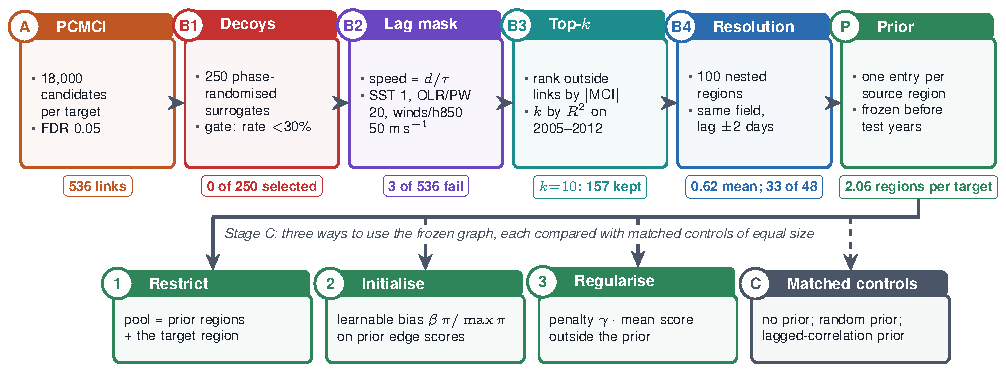
\includegraphics[width=\textwidth]{workflows/wf_validation.pdf}
\caption{Stage~B validation and Stage~C use of the graph. The tags under each check give the measured outcome (Chapter~\ref{chap:results}). The frozen region-level prior enters the splitter in one of three modes and is compared with matched controls of equal size.}
\label{fig:validation}
\end{figure}

\section{B1: Surrogate Decoys}
\label{sec:val-b1}

The first check asks whether the pipeline selects series merely because they have realistic memory. Decoys are phase-randomised copies of real nodes~\cite{theiler1992testing,schreiber2000surrogate}. A series $x_t$ is Fourier-transformed, its phases are replaced by independent uniform random phases, and it is transformed back:
\begin{equation}
  \tilde{x}_t=\frac{1}{n}\sum_f |\hat{x}_f|\,e^{i\theta_f}\,e^{2\pi i f t/n},\qquad \theta_f\sim\mathcal{U}[0,2\pi).
  \label{eq:phaserand}
\end{equation}
The decoy keeps the power spectrum, and therefore the autocorrelation including the 30--60-day BSISO peak, but has no real relationship with any node. 250 decoys are added to the 300 real nodes in a separate PCMCI pass (550 nodes, 33{,}000 candidates per target). The \emph{decoy rate} $\delta$ is the fraction of decoys selected as a parent of any target, and the pre-set warning line is $\delta\ge30\%$. Decoys do not reproduce non-Gaussian amplitudes, seasonal changes in variance, or a common driver shared with the target, so a low decoy rate rules out autocorrelation-driven selection but does not by itself prove causality.

\section{B2: Physical Lag Mask}
\label{sec:val-b2}

A link from region $r'$ to region $r$ at lag $\tau$ requires a signal to travel at least the closest great-circle distance $d(r',r)$ between the two regions in $\tau$ days. Its implied speed is
\begin{equation}
  s_e=\frac{d(r',r)}{\tau\times 86{,}400\,\mathrm{s}},
  \label{eq:speed}
\end{equation}
and the link fails if $s_e$ exceeds a generous limit for its source field: 1\ms\ for SST, whose own influence is ocean-mediated; 20\ms\ for OLR and PW, the upper range of convectively coupled Kelvin waves~\cite{kiladis2009convectively}; and 50\ms\ for the wind and height fields, which can be carried by fast equatorial waves. Unlike a distance cutoff, this test keeps remote teleconnections that act at plausible speeds. Links at lags of 25 days or more are flagged as possible echoes of the 30--60-day oscillation. Failing links are removed from the forecasting prior but kept, with their flags, in the graph file for inspection.

\section{B3: Data-Driven Top-\texorpdfstring{$k$}{k}}
\label{sec:val-b3}

Each target's outside links, those from other regions, are ranked by $|\hat\rho^{\,\mathrm{MCI}}|$. For each $k=0,\dots,10$, a ridge regression on the target's own-region links plus its top-$k$ outside links is fitted on 1979--2004 season days and scored by $R^2$ on 2005--2012; $k$ is chosen as the maximiser. The test period plays no part. The step sets the size of the prior from data and caps the number of drivers per target.

\section{B4: Resolution Persistence}
\label{sec:val-b4}

A link that is an artefact of how the regions were drawn should be fragile under a different partition. Stage~A is rerun at 100 nested regions (each region split in two). An outside link persists if some child pair carries a link from the same field at a lag within $\pm2$ days. The persistence score of target $r$ is the fraction of its outside links that persist, and a target passes if $\Pi_r\ge0.5$. Failures are flagged rather than deleted, because a real large-scale signal can be diluted at a finer scale.

\section{From Validated Links to a Region-Level Prior}
\label{sec:moe-prior}

The splitter chooses whole source regions, and the field chosen within a region is the least stable part of the graph. Validated outside links are therefore merged per source region:
\begin{equation}
  \pi_r(r')=\max_{e:\ \mathrm{src}(e)=r'}\ |\hat\rho^{\,\mathrm{MCI}}_e|,
  \label{eq:prior}
\end{equation}
over the links that pass B1 and B2 and survive B3. Field and lag details remain in the frozen graph file.

\section{The Graph-Guided Mixture of Experts}
\label{sec:moe-arch}

Each region has its own causal splitter and expert, 50 independent pairs trained from scratch with no weight sharing. Over time each region keeps a lineage of experts managed by the lifecycle of Section~\ref{sec:lifecycle}, which makes the system a Mixture of Experts in which a region's active expert can change with the regime~\cite{jacobs1991adaptive}.

\paragraph{Candidate pools.} The splitter of target $r$ considers either its adjacent regions (\emph{direct}, about 6--8), neighbours of neighbours (\emph{2hop}, about 15--23), or all 50 regions (\emph{full}). The target region is always a candidate.

\label{sec:moe-splitter}
\paragraph{Causal splitter.} Following DIR~\cite{wu2022discovering}, a rationale generator scores each candidate edge from a 10-day window of the two regions' histories,
\begin{equation}
  a_{r'r,t}=\sigma\big(\mathrm{MLP}[\mathbf{w}^{r'}_t\,\|\,\mathbf{w}^{r}_t]+b_{r'r}\big),
  \label{eq:score}
\end{equation}
where $b_{r'r}$ is an optional prior bias. The top fraction $\min(0.5,3/|\mathcal{C}_r|)$ of edges forms the causal set; the remaining edges are swapped with the same edges on $M=6$ other days to create interventions. The splitter minimises the mean and variance of the risk across interventions,
\begin{equation}
  \mathcal{L}_{\mathrm{split}}=\frac{1}{M}\sum_{m}\ell_{t,m}+\lambda\,\mathrm{Var}_m[\ell_{t,m}],
  \label{eq:dirloss}
\end{equation}
with $\lambda$ warmed up from 0 to 1. A spurious head with detached gradients serves as a leakage check.

\paragraph{Expert.} The expert aggregates the selected sources' 49-value feature vectors, weighted by their splitter scores, and maps the result to the forecast with a small MLP. The target's own history enters only if the target region is selected, so the forecast depends on the splitter's choice. A splitter is \emph{informative} if the spread of its candidates' mean scores is $\sigma_a\ge0.02$; below that the scores cluster around one value and the selection is effectively random.

\section{Three Ways to Use the Graph}
\label{sec:moe-modes}

\begin{itemize}
  \item \textbf{Restrict:} the candidate pool becomes the prior regions plus the target, $\mathcal{C}_r=\{r'\in\pi_r\}\cup\{r\}$.
  \item \textbf{Initialise:} the pool is unchanged, and the learnable bias in Eq.~\eqref{eq:score} starts at $b_{r'r}=2\,\pi_r(r')/\max\pi_r$ for prior regions and 0 otherwise.
  \item \textbf{Regularise:} the pool is unchanged, and a penalty $\gamma\cdot\mathrm{mean}(a_{r'r})$ over candidates outside the prior is added to the loss.
\end{itemize}
To attribute an effect to the graph's content, each mode is compared with matched controls of equal size per target: no prior, a random prior (the same number of regions drawn at random with the strengths shuffled), and a lagged-correlation prior (the regions most correlated with the target on training data).

A link at lag $\tau$ can inform a direct forecast at lead $L$ only if $\tau\ge L$, because the source value it describes must be known at the issue time. A graph whose links act within one or two days is therefore matched to short-lead forecasts.

\section{Drift Detection and the Expert Lifecycle}
\label{sec:lifecycle}

Figure~\ref{fig:lifecycle} shows how each region's expert is kept current.

\begin{figure}[htbp]
\centering
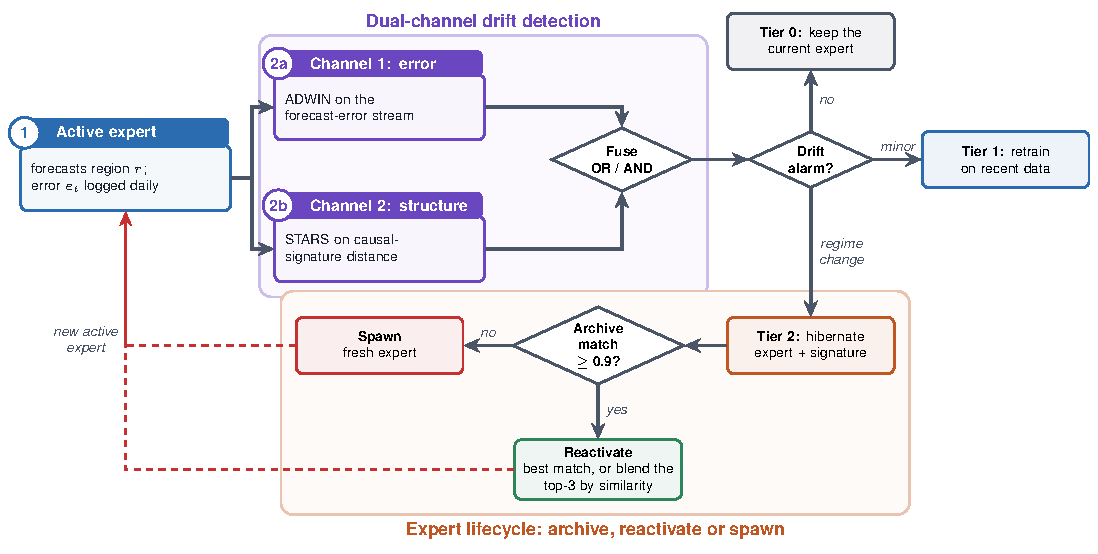
\includegraphics[width=\textwidth]{workflows/wf_lifecycle.pdf}
\caption{Drift detection and the expert lifecycle for one region. Two channels watch the forecast error and the causal structure; a fused alarm leads to retraining, or to archiving the expert and then reactivating a matching archived expert or spawning a fresh one.}
\label{fig:lifecycle}
\end{figure}

\paragraph{Channel 1: error (ADWIN).} ADWIN~\cite{bifet2007learning} keeps an adaptive window of recent forecast errors. Whenever two sub-windows have significantly different mean errors, it drops the older part and raises an alarm. For a window $W$ split into sub-windows $W_0$ and $W_1$ with means $\hat\mu_0,\hat\mu_1$ and sizes $n_0,n_1$, a change is declared if
\begin{equation}
  |\hat\mu_0-\hat\mu_1|>\epsilon_{\mathrm{cut}}=\sqrt{\frac{1}{2m}\ln\frac{4|W|}{\delta}},\qquad m=\Big(\frac{1}{n_0}+\frac{1}{n_1}\Big)^{-1},
\end{equation}
where $\delta$ is the confidence parameter.

\paragraph{Channel 2: causal structure (STARS).} The splitter's per-edge score vector on each day is the region's causal signature; its cosine distance from a reference signature (the mean over a baseline window) forms a scalar causal-structure series. Rodionov's STARS test~\cite{rodionov2004sequential} flags a point that falls outside the current regime's range and confirms a shift only if the following $\ell$ points support the new level. For a candidate shift at time $j$, the regime-shift index
\begin{equation}
  \mathrm{RSI}_j=\sum_{i=j}^{j+m}\frac{x_i-\bar{x}_{\mathrm{crit}}}{\ell\,\hat\sigma_\ell},\qquad m=0,\dots,\ell-1,
\end{equation}
must keep its sign over the cut-off length $\ell$, where $\bar{x}_{\mathrm{crit}}$ is the level that a new regime's mean must exceed at the chosen significance and $\hat\sigma_\ell$ is the average standard deviation over intervals of length $\ell$. Because it watches the structure rather than the outcome, it can in principle detect a change before forecasts degrade.

\paragraph{Fusion.} The channels are combined with OR, which reacts faster but raises more alarms, or with AND, which is slower but has fewer false alarms.

\paragraph{Lifecycle.} After an alarm, a minor change triggers retraining (Tier~1). A regime change (Tier~2) hibernates the current expert together with its causal signature and searches the archive. If an archived expert's signature has cosine similarity of at least 0.9, it is reactivated, either the single best match or a similarity-weighted blend of the three best matches; otherwise a fresh expert is spawned. Because climate regimes such as ENSO phases recur, reactivation reuses knowledge instead of relearning it, and adding experts rather than overwriting them limits catastrophic forgetting~\cite{kirkpatrick2017overcoming}.

\paragraph{Stage D: structural drift of the PCMCI graph.} Separately, PCMCI is rerun on sliding windows of one or three BSISO seasons, restricted to each target's B1/B2-validated candidates. The distance $\Delta_w=1-J(\mathcal{P}_w,\mathcal{P}_{w-1})$ between consecutive parent sets, where $J$ is the Jaccard similarity, is tested with STARS and compared with ENSO phase changes derived from the project's own SST.

\section{Consolidated Algorithm}
\label{sec:moe-algorithm}

Algorithm~\ref{alg:build-validate} summarises Phase~1. Every step before the freeze uses 1979--2012 only.

\begin{algorithm}[htbp]
\caption{Build, validate, freeze and use the causal graph, and keep experts current}
\label{alg:build-validate}
\small
\begin{algorithmic}[1]
\State compute the BSISO index and season $\mathcal{S}$ (EOF fitted on 1979--2012)
\State \textbf{Stage A:} run PCMCI (Algorithm~\ref{alg:pcmci}) for each of the 50 OLR targets
\State \textbf{B1:} add 250 phase-randomised decoys in a separate pass; stop if the decoy rate is $\ge 30\%$
\State \textbf{B2:} compute implied speeds; remove links above the field's limit from the prior
\State \textbf{B3:} choose $k$ by validation $R^2$; keep the top-$k$ outside links per target
\State \textbf{B4:} rerun PCMCI at 100 regions; flag targets with $\Pi_r<0.5$
\State build the region prior $\pi_r$ (Eq.~\ref{eq:prior}) and \textbf{freeze} graph and prior
\State \textbf{Stage C:} train a splitter and expert per region with the prior (restrict, initialise or regularise) and with matched controls; score on 2013--2022
\For{each day in the monitored period} \Comment{lifecycle}
  \State update ADWIN (error) and STARS (structure); fuse with OR or AND
  \If{alarm} retrain, or hibernate and reactivate a matching archived expert (similarity $\ge 0.9$), or spawn
  \EndIf
\EndFor
\State \textbf{Stage D:} sliding-window PCMCI, $\Delta_w$, STARS and comparison with ENSO
\end{algorithmic}
\end{algorithm}

\chapter{Implementation and Experimental Design}
\label{chap:experiments}

\section{Software and Computational Environment}
\label{sec:impl-env}

The system is implemented in Python as a library (\texttt{causal\_moe}) with one runnable script per experiment and an automated test suite. All experiments run on CPU. Table~\ref{tab:software} lists the main dependencies with the versions pinned in the project's requirements file.

\begin{table}[htbp]
\centering
\caption{Software environment (versions as pinned in \texttt{code/requirements.txt}).}
\label{tab:software}
\footnotesize
\renewcommand{\arraystretch}{1.15}
\begin{tabularx}{\textwidth}{>{\raggedright\arraybackslash}p{3.6cm}>{\raggedright\arraybackslash}p{2.0cm}>{\raggedright\arraybackslash}X}
\toprule
\textbf{Component} & \textbf{Version} & \textbf{Use} \\
\midrule
NumPy~\cite{harris2020array} & 1.26.4 & Arrays, FFT surrogates, vectorised PCMCI \\
SciPy~\cite{virtanen2020scipy} & 1.17.1 & Student-$t$ distribution, statistical tests \\
pandas & 2.3.3 & Calendar handling, season construction \\
scikit-learn~\cite{pedregosa2011scikit} & 1.9.0 & $k$-means partition \\
PyTorch~\cite{paszke2019pytorch} (CPU) & 2.13.0 & Splitter and expert models \\
PyTorch Geometric~\cite{fey2019fast} & 2.8.0 & Message passing on the region graph \\
river~\cite{montiel2021river} & 0.22.0 & ADWIN error-stream drift detector \\
Matplotlib & 3.11.0 & Figures \\
pytest & 9.0.3 & Automated tests \\
Tigramite & 5.2.10.1 & Reference PCMCI for verification only \\
\bottomrule
\end{tabularx}
\end{table}

\section{Data Pipeline and Preprocessing}
\label{sec:impl-data}

The data pipeline consists of four modules. \texttt{data/raw.py} loads the six gridded anomaly fields and the ocean mask into a single array of shape $(6, 16071, 25, 144)$. \texttt{data/clustering.py} builds the 50-region partition by $k$-means on OLR, and \texttt{data/mesh.py} derives the adjacency of regions, with longitude wrap-around. \texttt{causal\_graph/nodes.py} forms the 300 regional-mean node series (SST over ocean cells only), re-standardises each node over 1979--2012, constructs the nested 100-region split, and computes closest-cell haversine distances between all pairs of regions. \texttt{causal\_graph/season.py} computes the BSISO index and the per-year season mask. \texttt{data/windows.py} builds the 49-dimensional feature vectors and lead-$L$ targets and caches them to disk, so that all forecasting experiments read identical inputs.

\section{PCMCI Implementation and Verification}
\label{sec:impl-pcmci}

\texttt{causal\_graph/pcmci.py} implements Algorithm~\ref{alg:pcmci}. The lagged design for all 300 nodes at 60 lags on the 7{,}153 season target days is built once ($7{,}153\times 18{,}000$ single-precision values, about 0.5\,GB) and shared by all targets. Partial correlations are computed by orthonormalising the conditioning set with a QR decomposition and residualising all candidate columns in one matrix product, processed in chunks of 4{,}096 columns.

Correctness was verified by dedicated tests (\texttt{tests/test\_pcmci.py}) on synthetic vector-autoregressive data with known parents, including a common driver and a pure-noise node. The tests check that the implementation recovers the true parents and rejects the common-driver and noise nodes, and they compare it with Tigramite's \texttt{PCMCI.run\_pcmci} using ParCorr and equivalent link assumptions (any lagged parent for the targets; own past only for the other nodes), for one target and for two targets that are also sources of each other. The PC1 parent sets must be identical, the MCI strengths must agree to within $2\times10^{-3}$ and the $p$-values to within 5\% relative error. All tests pass. The full 50-target Stage~A run then takes about 23 minutes on a multi-core CPU. Table~\ref{tab:pcmci-config} gives the configuration.

\begin{table}[htbp]
\centering
\caption{Stage~A (PCMCI) configuration as recorded in the frozen graph file.}
\label{tab:pcmci-config}
\footnotesize
\renewcommand{\arraystretch}{1.15}
\begin{tabular}{p{6.5cm}p{4.5cm}p{3.3cm}}
\toprule
\textbf{Parameter} & \textbf{50 regions} & \textbf{100 regions (B4)} \\
\midrule
Nodes & 300 & 596 \\
Candidates per target & 18{,}000 & 35{,}760 \\
Targets & 50 OLR nodes & 100 OLR nodes \\
Target days & \multicolumn{2}{l}{7{,}153 season days, 1979--2012} \\
Lags $\taumin$--$\taumax$ & \multicolumn{2}{l}{1--60 days (lag 0 excluded)} \\
CI test & \multicolumn{2}{l}{ParCorr (partial correlation, Student-$t$)} \\
$\alpha_{\mathrm{PC}}$ & \multicolumn{2}{l}{0.05} \\
PC1 combinations per iteration & \multicolumn{2}{l}{1} \\
Max.\ conditioning dimension & \multicolumn{2}{l}{unlimited} \\
Non-target node parents & \multicolumn{2}{l}{own past only} \\
Multiple-testing correction & \multicolumn{2}{l}{Benjamini--Hochberg over all candidates per target} \\
$\alpha_{\mathrm{FDR}}$ & \multicolumn{2}{l}{0.05} \\
\bottomrule
\end{tabular}
\end{table}

\section{Surrogate Generation}
\label{sec:impl-surrogates}

\texttt{causal\_graph/validate.py} generates decoys with NumPy's real FFT: the demeaned series is transformed, the zero-frequency phase (and the Nyquist phase for an even length) is fixed at zero, the remaining phases are drawn from $\mathcal{U}[0,2\pi)$, the inverse transform is taken, and the result is standardised (Eq.~\eqref{eq:phaserand}). The 250 decoys are built from real source nodes drawn with replacement, using a fixed random seed, and the origin of every decoy is recorded. The decoy pass reuses the PCMCI implementation with the 550-node pool; decoy links are marked with a source region of $-1$.

\section{Physical-Mask Implementation}
\label{sec:impl-mask}

Closest-cell distances are precomputed for all region pairs from cell-centre coordinates with the haversine formula. For each link, the implied speed of Eq.~\eqref{eq:speed}, the pass/fail result against the limits in Table~\ref{tab:speeds}, and the oscillation flag for $\tau\ge 25$ days are added to the link record.

\section{Top-\texorpdfstring{$k$}{k} Selection and Resolution Comparison}
\label{sec:impl-topk}

The top-$k$ search evaluates $k=0,\dots,10$ by ridge regression with constant $10^{-3}$, fitted on 1979--2004 and scored on 2005--2012 season days (Eq.~\eqref{eq:r2k}). The resolution comparison reruns Stage~A on the 100-region nodes and evaluates the persistence rule of Eq.~\eqref{eq:persist} with a lag tolerance of $\pm2$ days. The frozen output, \texttt{results/phase1/causal\_graph\_50.json}, holds the configuration of every stage, the summary statistics, and for each target its validated links (source region, field, lag, strength, $p$, $q$, distance, speed and all flags) together with the region-level prior. Table~\ref{tab:val-config} gives the validation configuration.

\begin{table}[htbp]
\centering
\caption{Stage~B configuration.}
\label{tab:val-config}
\footnotesize
\renewcommand{\arraystretch}{1.15}
\begin{tabularx}{\textwidth}{>{\raggedright\arraybackslash}p{4.0cm}>{\raggedright\arraybackslash}X}
\toprule
\textbf{Check} & \textbf{Setting} \\
\midrule
B1 decoys & 250 phase-randomised surrogates; separate PCMCI pass (550 nodes, 33{,}000 candidates per target); warning line: decoy rate $\ge 30\%$; strength bar: strongest selected decoy \\
B2 lag mask & Closest-cell haversine distance; limits SST 1\ms, OLR and PW 20\ms, h850, u850 and u200 50\ms; flag $\tau\ge 25$ days; failures removed from the prior, kept in the graph file \\
B3 top-$k$ & Outside links ranked by $|\MCI|$; $k\in\{0,\dots,10\}$; ridge fit 1979--2004, $R^2$ on 2005--2012 season days \\
B4 persistence & 100 nested regions ($k$-means, 2 per region); same field, lag within $\pm 2$ days, any child pair; pass if $\Pi_r\ge 0.5$; flag only \\
Prior & One entry per source region, strength $=\max|\MCI|$ \\
\bottomrule
\end{tabularx}
\end{table}

\section{MoE Integration}
\label{sec:impl-moe}

The splitter (\texttt{splitter/dirgnn.py}) and the expert (\texttt{experts/expert.py}) are trained jointly with one Adam optimiser. \texttt{causal\_graph/prior.py} builds the priors (\texttt{pcmci}, \texttt{random}, \texttt{corr}) and applies the modes (\texttt{restrict}, \texttt{init}, \texttt{regularize}). All prior options are off by default, so that the earlier, prior-free behaviour is reproduced exactly when no prior is requested. Table~\ref{tab:hyper} lists the training configuration, which is identical for every condition compared in this thesis.

\begin{table}[htbp]
\centering
\caption{Splitter and expert training configuration, identical across all compared conditions.}
\label{tab:hyper}
\footnotesize
\renewcommand{\arraystretch}{1.15}
\begin{tabular}{p{7.0cm}p{6.5cm}}
\toprule
\textbf{Setting} & \textbf{Value} \\
\midrule
Epochs & 5 \\
Training samples & first 4{,}000 contiguous season samples of the training period \\
Optimiser, learning rate & Adam, $10^{-3}$ \\
Batch size & 16 \\
Hidden width (splitter encoder, expert MLP) & 16 \\
Rationale generator window & 10 days \\
Interventions per sample $M$ & 6 \\
Variance weight $\lambda$ & 0 for the first 30\% of steps, then linear ramp to 1 \\
Selected fraction $\rho_{\mathrm{top}}$ & $\min(0.5,\;3/|\mathcal{C}_r|)$ \\
Target's own features supplied unconditionally & no (only if selected) \\
Initialise-mode scale $\beta$ & 2 \\
Regularise-mode weight $\gamma$ & 1 \\
Informative-splitter threshold on $\sigma_a$ & 0.02 \\
Seed & 0 \\
Lead times & 7 days (primary), 1 day (secondary) \\
Train / validation / test & 1979--2004 / 2005--2012 / 2013--2022 \\
Scored test days & 1{,}989 season target days \\
\bottomrule
\end{tabular}
\end{table}

\section{Experimental Conditions and Ablations}
\label{sec:exp-grid}

The Stage~C design crosses three priors (\texttt{pcmci}, \texttt{random}, \texttt{corr}) with three modes (restrict, initialise, regularise) and three pools (direct, 2hop, full), giving 27 prior configurations, plus a no-prior baseline per pool. Each configuration trains one splitter and expert per region, 50 per configuration, or 1{,}350 trainings for the prior grid. Table~\ref{tab:grid} shows the grid and the configurations reported in this thesis.

\begin{table}[htbp]
\centering
\caption{Stage~C experimental grid. \done\ = results reported in Chapter~\ref{chap:results}; \planned\ = defined, implemented and unit-tested, results to follow. All cells use identical data, splits, seed and training budget.}
\label{tab:grid}
\footnotesize
\renewcommand{\arraystretch}{1.2}
\begin{tabular}{llccc}
\toprule
\textbf{Prior} & \textbf{Mode} & \textbf{direct} & \textbf{2hop} & \textbf{full} \\
\midrule
none & -- & \done\ (7\,d) & \done\ (7\,d) & \done\ (7\,d, 1\,d) \\
pcmci & restrict & \planned & \planned & \done\ (7\,d, 1\,d) \\
pcmci & initialise & \planned & \planned & \planned \\
pcmci & regularise & \planned & \planned & \planned \\
random & restrict / initialise / regularise & \planned & \planned & \planned \\
corr & restrict / initialise / regularise & \planned & \planned & \planned \\
\bottomrule
\end{tabular}
\end{table}

The full pool is the most informative setting for the first comparison, because it is the one in which the splitter alone fails to discriminate (Section~\ref{sec:res-pool}) and in which a prior has the most room to help. The restrict mode is the strongest form of the prior. The reported comparisons are therefore the most direct test of whether the validated graph can rescue source selection in a large pool. The random-prior control at the same pool and mode is the next comparison in the programme, because it separates the effect of the graph's content from the effect of a smaller pool. Further ablations defined for the graph itself are listed in Appendix~\ref{app:registry}: the graph rebuilt with $\taumin=7$, top-$k$ selected by forecast-horizon skill, a full-year graph, persistence across the two halves of the development period, and a second data source.

\section{Train, Validation and Holdout Discipline}
\label{sec:exp-discipline}

Every decision that could be tuned (the season definition, the PCMCI parameters, the validation thresholds, the choice of $k$ and the training configuration) was fixed using 1979--2012 data only, and the graph was frozen before any forecast on 2013--2022 was scored. Test-period scores were not used to select among configurations. Each reported configuration is a pre-defined cell of the grid in Table~\ref{tab:grid}.

\section{Metrics}
\label{sec:exp-metrics}

\subsection{Forecast accuracy}
For region $r$ with test days $t\in\mathcal{T}_r$ and forecasts $\hat{Y}_t$ of targets $Y_t$ (lead suppressed for brevity):
\begin{align}
  \MSE &= \frac{1}{|\mathcal{T}_r|}\sum_t(\hat{Y}_t-Y_t)^2, &
  \mathrm{RMSE} &= \sqrt{\MSE}, &
  \mathrm{MAE} &= \frac{1}{|\mathcal{T}_r|}\sum_t|\hat{Y}_t-Y_t|.
  \label{eq:mse}
\end{align}
Because the target is a standardised anomaly, these errors are in units of the target's development-period standard deviation.

\subsection{Skill scores}
Skill is measured relative to two reference forecasts~\cite{murphy1988skill,jolliffe2012forecast}. \emph{Persistence} predicts that the anomaly at the issue time persists, $\hat{Y}^{\mathrm{pers}}_{t+L}=Y_t$. \emph{Climatology} predicts the mean of the training targets, $\hat{Y}^{\mathrm{clim}}=\bar{Y}_{\mathrm{train}}$, which is close to zero for anomalies. The MSE skill scores are
\begin{equation}
  S_{\mathrm{pers}} = 1-\frac{\MSE}{\MSE_{\mathrm{pers}}},\qquad
  R^2_{\mathrm{clim}} = 1-\frac{\MSE}{\MSE_{\mathrm{clim}}}.
  \label{eq:skill}
\end{equation}
A positive score means the model beats the reference. The two references are complementary. At short leads persistence is very hard to beat and climatology easy; at seven days OLR keeps almost no memory, so persistence becomes a weak reference, while climatology, which is the optimal constant forecast under squared error, becomes the demanding one. Both scores are reported together. The anomaly correlation coefficient
\begin{equation}
  \mathrm{ACC} = \frac{\sum_t(\hat{Y}_t-\bar{\hat{Y}})(Y_t-\bar{Y})}{\sqrt{\sum_t(\hat{Y}_t-\bar{\hat{Y}})^2\sum_t(Y_t-\bar{Y})^2}}
\end{equation}
measures phase agreement independently of amplitude and is part of the evaluation set for future runs.

\subsection{Source-selection quality}
The splitter's discrimination is measured by $\sigma_a$, the standard deviation of a target's mean candidate scores over the test days, and summarised as the number of informative splitters ($\sigma_a\ge 0.02$) out of 50. The selected sources and their overlap with the prior are recorded for every region.

\subsection{Graph metrics}
Stage~A and B are summarised by link counts by field, region and lag, the decoy rate, the number of B2 failures, the validation $R^2$ curve, the persistence scores, the prior size per target and the Jaccard distance between windows (Section~\ref{sec:val-metrics}).

\section{Statistical Analysis}
\label{sec:exp-stats}

Comparisons between two conditions are \emph{paired}: both are evaluated on the same 50 regions and the same test days. For each region the difference of a score between the two conditions is computed, and the distribution of the 50 differences is summarised by the number of regions that improve, the median and the mean. Two tests of a zero median difference are reported: the sign test, which uses only the direction of each difference, and the Wilcoxon signed-rank test, which also uses their ranks. These tests treat regions as independent, which they are not: neighbouring regions share weather and their errors are correlated. Their $p$-values are therefore indicative and likely too small.

Temporal dependence within a region matters for any test performed on daily errors. Consecutive forecast errors are autocorrelated, so a test that treats the 1{,}989 test days as independent would overstate significance~\cite{wilks1997resampling}. The appropriate tools are the Diebold--Mariano test with a heteroscedasticity- and autocorrelation-consistent variance~\cite{diebold1995comparing} for paired error series, and the moving-block bootstrap~\cite{kunsch1989jackknife} for confidence intervals of skill scores. Variability due to training randomness is measured by repeating each configuration over several seeds. These analyses are part of the evaluation protocol for the full grid; the comparisons reported in this thesis use a single seed and are interpreted accordingly. Results that are neutral or negative are reported with the same detail as positive ones.

\section{Runtime, Memory and Scalability}
\label{sec:exp-runtime}

Table~\ref{tab:runtime} gives approximate wall-clock costs on the project's CPU workstation. The dominant cost of Stage~C is the number of trainings, $3\times3\times3\times50=1{,}350$ for the full grid, which runs in parallel across regions.

\begin{table}[htbp]
\centering
\caption{Approximate wall-clock costs (CPU only).}
\label{tab:runtime}
\footnotesize
\renewcommand{\arraystretch}{1.15}
\begin{tabularx}{\textwidth}{>{\raggedright\arraybackslash}X>{\raggedright\arraybackslash}p{6.0cm}}
\toprule
\textbf{Step} & \textbf{Cost} \\
\midrule
Stage A, 50 regions (18{,}000 candidates $\times$ 50 targets) & about 23 min \\
Stages A + B in full (season, A50, decoy pass, A100, validation) & about 2.3--2.5 h on 20 threads \\
One Stage C configuration (50 regions) & about 20 min on 12 worker processes \\
One region, one configuration & roughly 0.5--1.5 min \\
Full Stage C grid (27 configurations) & about 6--8 h on 12 worker processes \\
Stage D, one window length & about 1 h \\
\bottomrule
\end{tabularx}
\end{table}

\section{Reproducibility and Artifact Organisation}
\label{sec:exp-repro}

All results are produced by scripts and saved as JSON files with their configuration; figures are regenerated from these files without retraining. The Phase~1 commands are:
\begin{lstlisting}
python scripts/phase1_build_graph.py        # season, A50, B1, A100, validation
python scripts/phase1_run_stage_c.py --pools full --priors none,pcmci --modes restrict
python scripts/phase1_run_stage_c.py --pools full --priors none,pcmci --modes restrict \
    --cache-path cache/windowed_clustered50_lead1_v2.npz --out-dir results/phase1/stage_c_lead1
python scripts/phase1_stage_d_drift.py --window-seasons 1
python scripts/phase1_stage_d_drift.py --window-seasons 3
python scripts/generate_phase1_figures.py
\end{lstlisting}
Appendix~\ref{app:repro} lists the repository structure, the result files behind every number in Chapter~\ref{chap:results}, and step-by-step instructions.

\section{Chapter Summary}
\label{sec:exp-summary}

This chapter described the software, the data pipeline, the verified vectorised PCMCI, the decoy, mask, top-$k$ and persistence implementations, and the integration of the prior into the splitter. It defined the 27-configuration Stage~C grid and identified the configurations reported here, the metrics for forecast skill and source selection, the paired statistical analysis and its limits, and the computational costs. The next chapter presents the results.

\chapter{Results and Discussion}
\label{chap:results}

This chapter reports the Phase~1 results in the order of the research questions. Every number comes from a saved result file of the project (Appendix~\ref{app:repro}).

\section{BSISO Season}
\label{sec:res-season}

The BSISO index reproduced from the project's own OLR and u850 anomalies has leading modes explaining 11.2\% and 7.7\% of the variance, close to the approximately 10\% and 7\% reported by Lee \emph{et al.}~\cite{lee2013realtime}. The slightly larger values are consistent with the smaller domain, whose northern edge is 30\dg N rather than 40\dg N. The activity-based season (Figure~\ref{fig:season}) lasts 208 days per year on average, ranges from 82 to 286 days, and begins between April and July. A fixed May--October window would therefore include inactive weeks in some years and miss active weeks in others.

\begin{figure}[htbp]
\centering
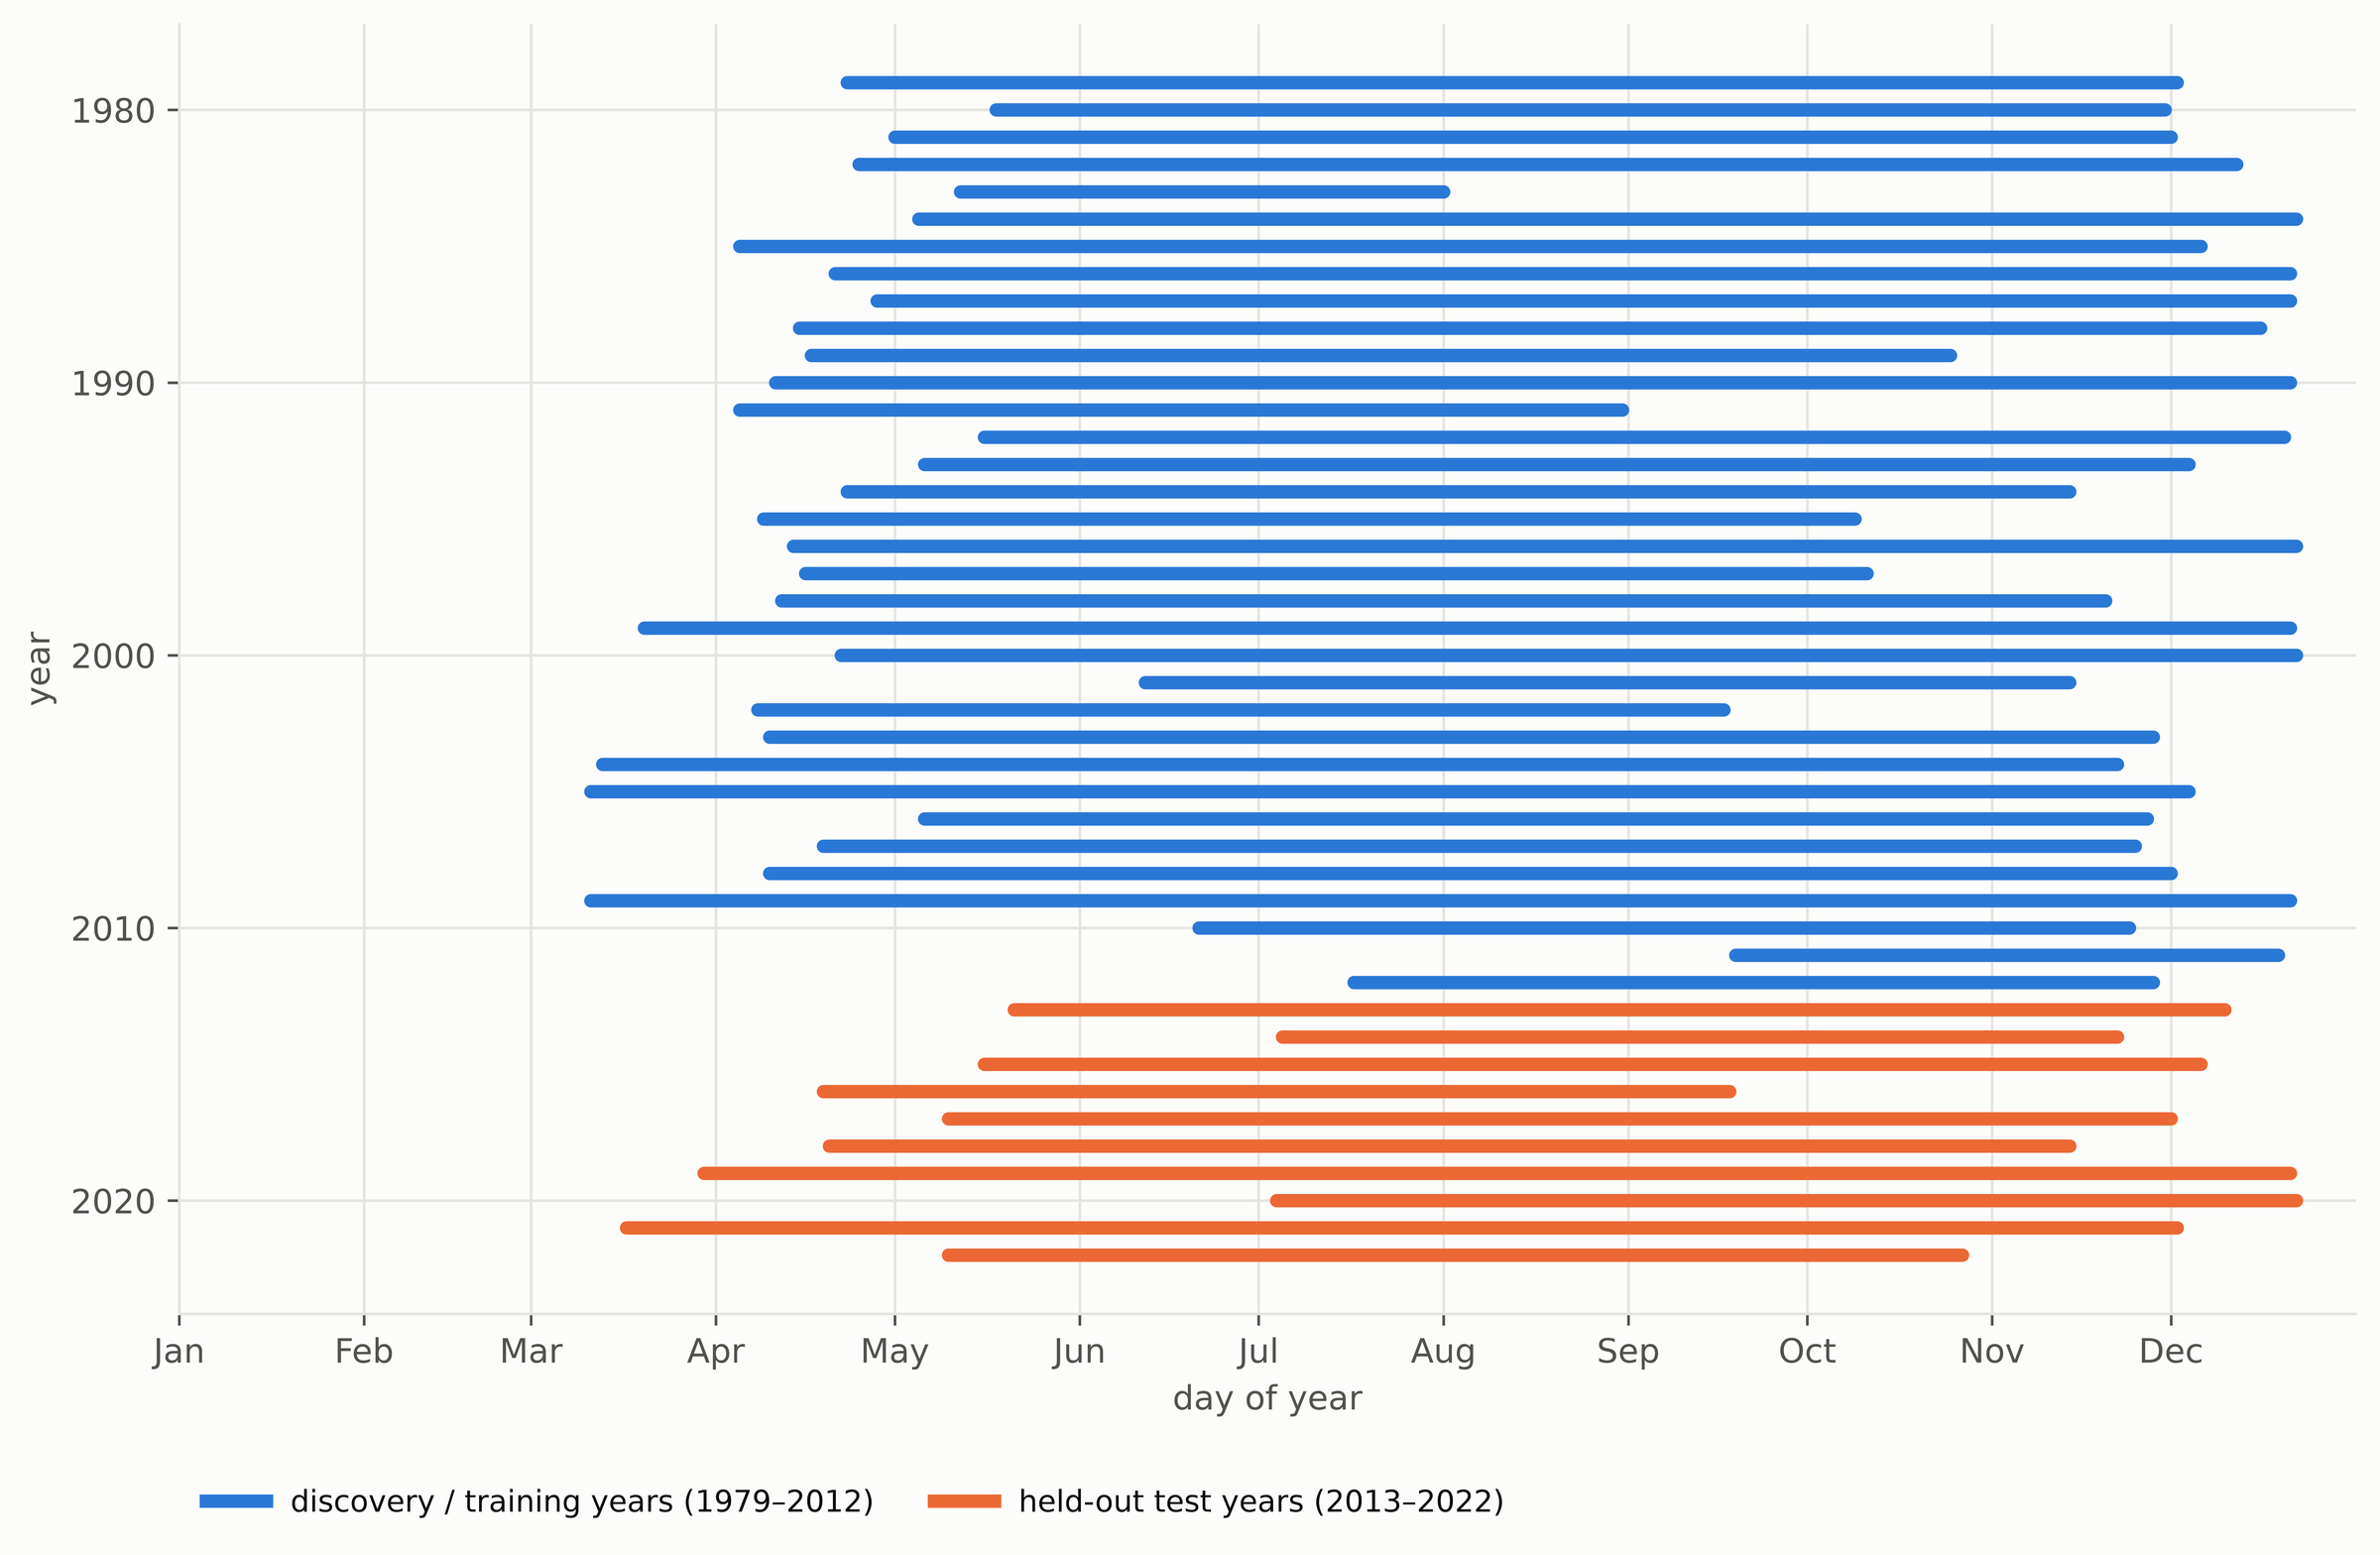
\includegraphics[width=0.82\textwidth]{ppt_01b_active_bsiso_season_per_year.png}
\caption{Active BSISO season (target days) in each year, derived from the reproduced BSISO index. Blue: discovery and training years (1979--2012); orange: held-out test years (2013--2022).}
\label{fig:season}
\end{figure}

\section{Stage A: The Discovered Graph (RQ1)}
\label{sec:res-stagea}

PCMCI at an FDR of 0.05 retains \textbf{536 links} into the 50 OLR targets, 10.7 per target, out of 900{,}000 candidates: the graph is very sparse. Of these, 376 lie within the target's own region, mostly its own OLR at lags of 1--7 days, and 160 come from other regions: OLR 72, u850 37, u200 22, h850 18, PW 11 and SST 0. The outside links act quickly, with a median lag of one day, 90\% at two days or less, and none at 25 days or more. Once PCMCI conditions on these fast drivers, slow precursors such as SST carry little \emph{direct} information, because their influence has already passed through the atmospheric fields. Convection in a neighbouring region, together with the low-level flow that carries moisture and the upper-level wave response, precedes convection in the target, which is the expected physical picture of propagating convection.

Figure~\ref{fig:graphmap} maps the outside drivers. Most connect neighbouring regions; a few longer links carried by wind and height fields span thousands of kilometres within one or two days, at equatorial-wave speeds.

\begin{figure}[htbp]
\centering
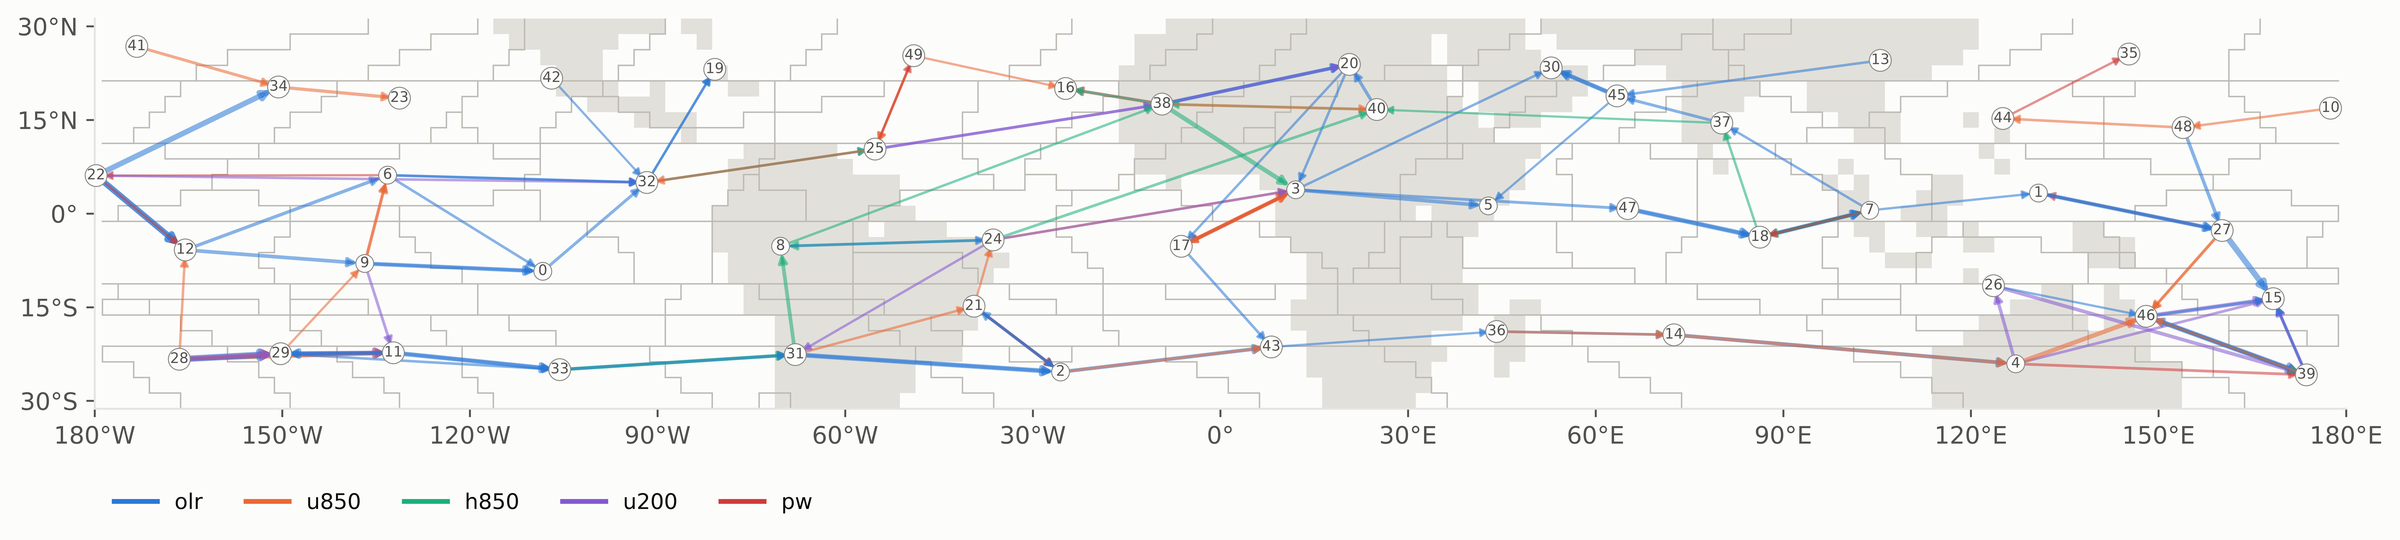
\includegraphics[width=\textwidth]{ppt_map_standard_180_convention.png}
\caption{Validated outside drivers of the 50 OLR targets (arrows from source region to target region), coloured by the source field.}
\label{fig:graphmap}
\end{figure}

\paragraph{Worked example: region 22.} Region 22 lies over the equatorial western Pacific near the Maritime Continent. PCMCI finds 13 links for it: 10 within the region and three from outside (h850 from region 27 at lags 1 and 3, and PW from region 6 at lag 2). Both source regions are about 280\,km away, so the implied speeds of 1--3\ms\ are physically easy. The prior is region 27 (strength 0.21) and region 6 (0.05). Independently, the splitter trained with no prior selects regions 6, 12 and 27, which include both prior regions: two unrelated methods agree on the same drivers. Table~\ref{tab:region22} follows the region's links through the checks.

\begin{table}[htbp]
\centering
\caption{The links of target region 22 through Stages A and B.}
\label{tab:region22}
\footnotesize
\renewcommand{\arraystretch}{1.15}
\begin{tabularx}{\textwidth}{>{\raggedright\arraybackslash}p{2.3cm}>{\centering\arraybackslash}p{1.6cm}>{\raggedright\arraybackslash}X}
\toprule
\textbf{Step} & \textbf{Links} & \textbf{What happened} \\
\midrule
PCMCI & 13 & 10 own-region (OLR lags 1--3, 5--7; u850, h850 lags 1--2); h850 from region 27 (lags 1, 3); PW from region 6 (lag 2) \\
B1 decoys & 13 & no decoy selected anywhere \\
B2 lag mask & 13 & sources $\approx$280\,km away; 1--3\ms \\
B3 top-$k$ & 3 outside & all three outside links kept \\
B4 persistence & 0.67 & both region-27 links persist; region-6 PW link flagged \\
Prior & 2 regions & region 27 (0.21), region 6 (0.05) \\
\bottomrule
\end{tabularx}
\end{table}

\section{Stage B: Validation (RQ2)}
\label{sec:res-stageb}

\begin{figure}[htbp]
\centering
\begin{subfigure}[b]{0.56\textwidth}\centering
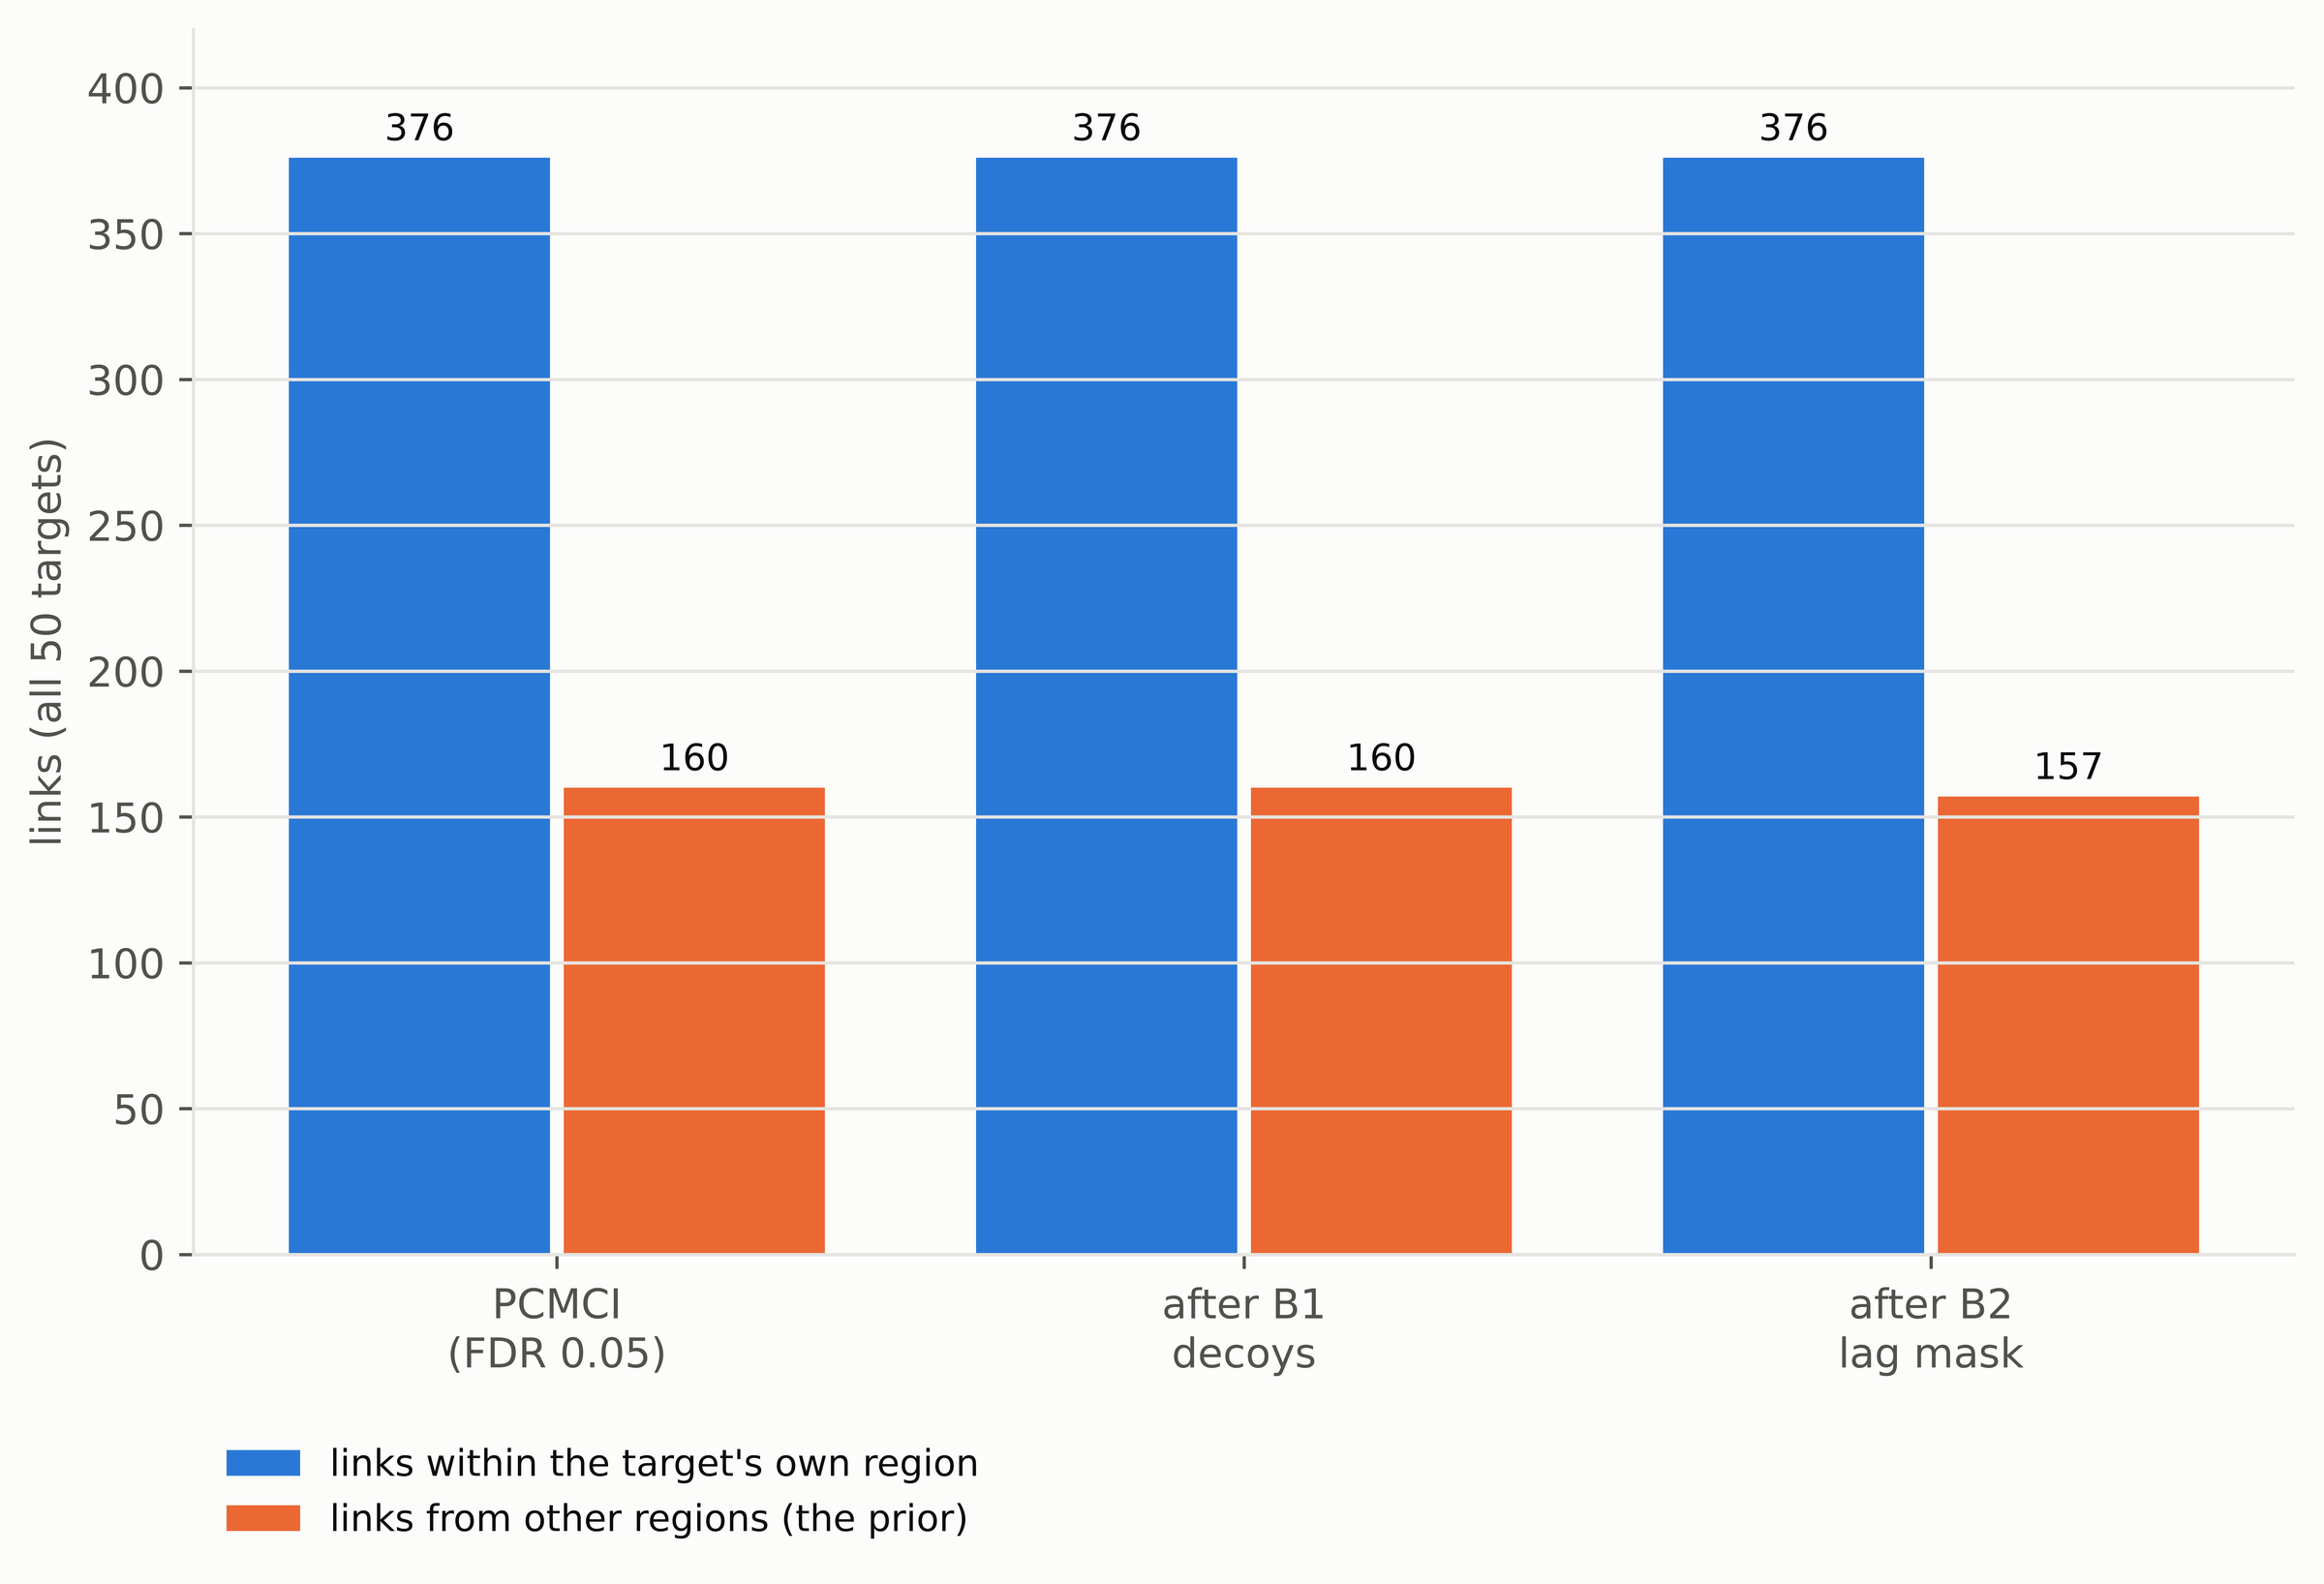
\includegraphics[width=\textwidth]{ppt_03b_links_through_checks_no_b3_b4.png}
\caption{Links after PCMCI, B1 and B2.}\label{fig:links}
\end{subfigure}\hfill
\begin{subfigure}[b]{0.4\textwidth}\centering
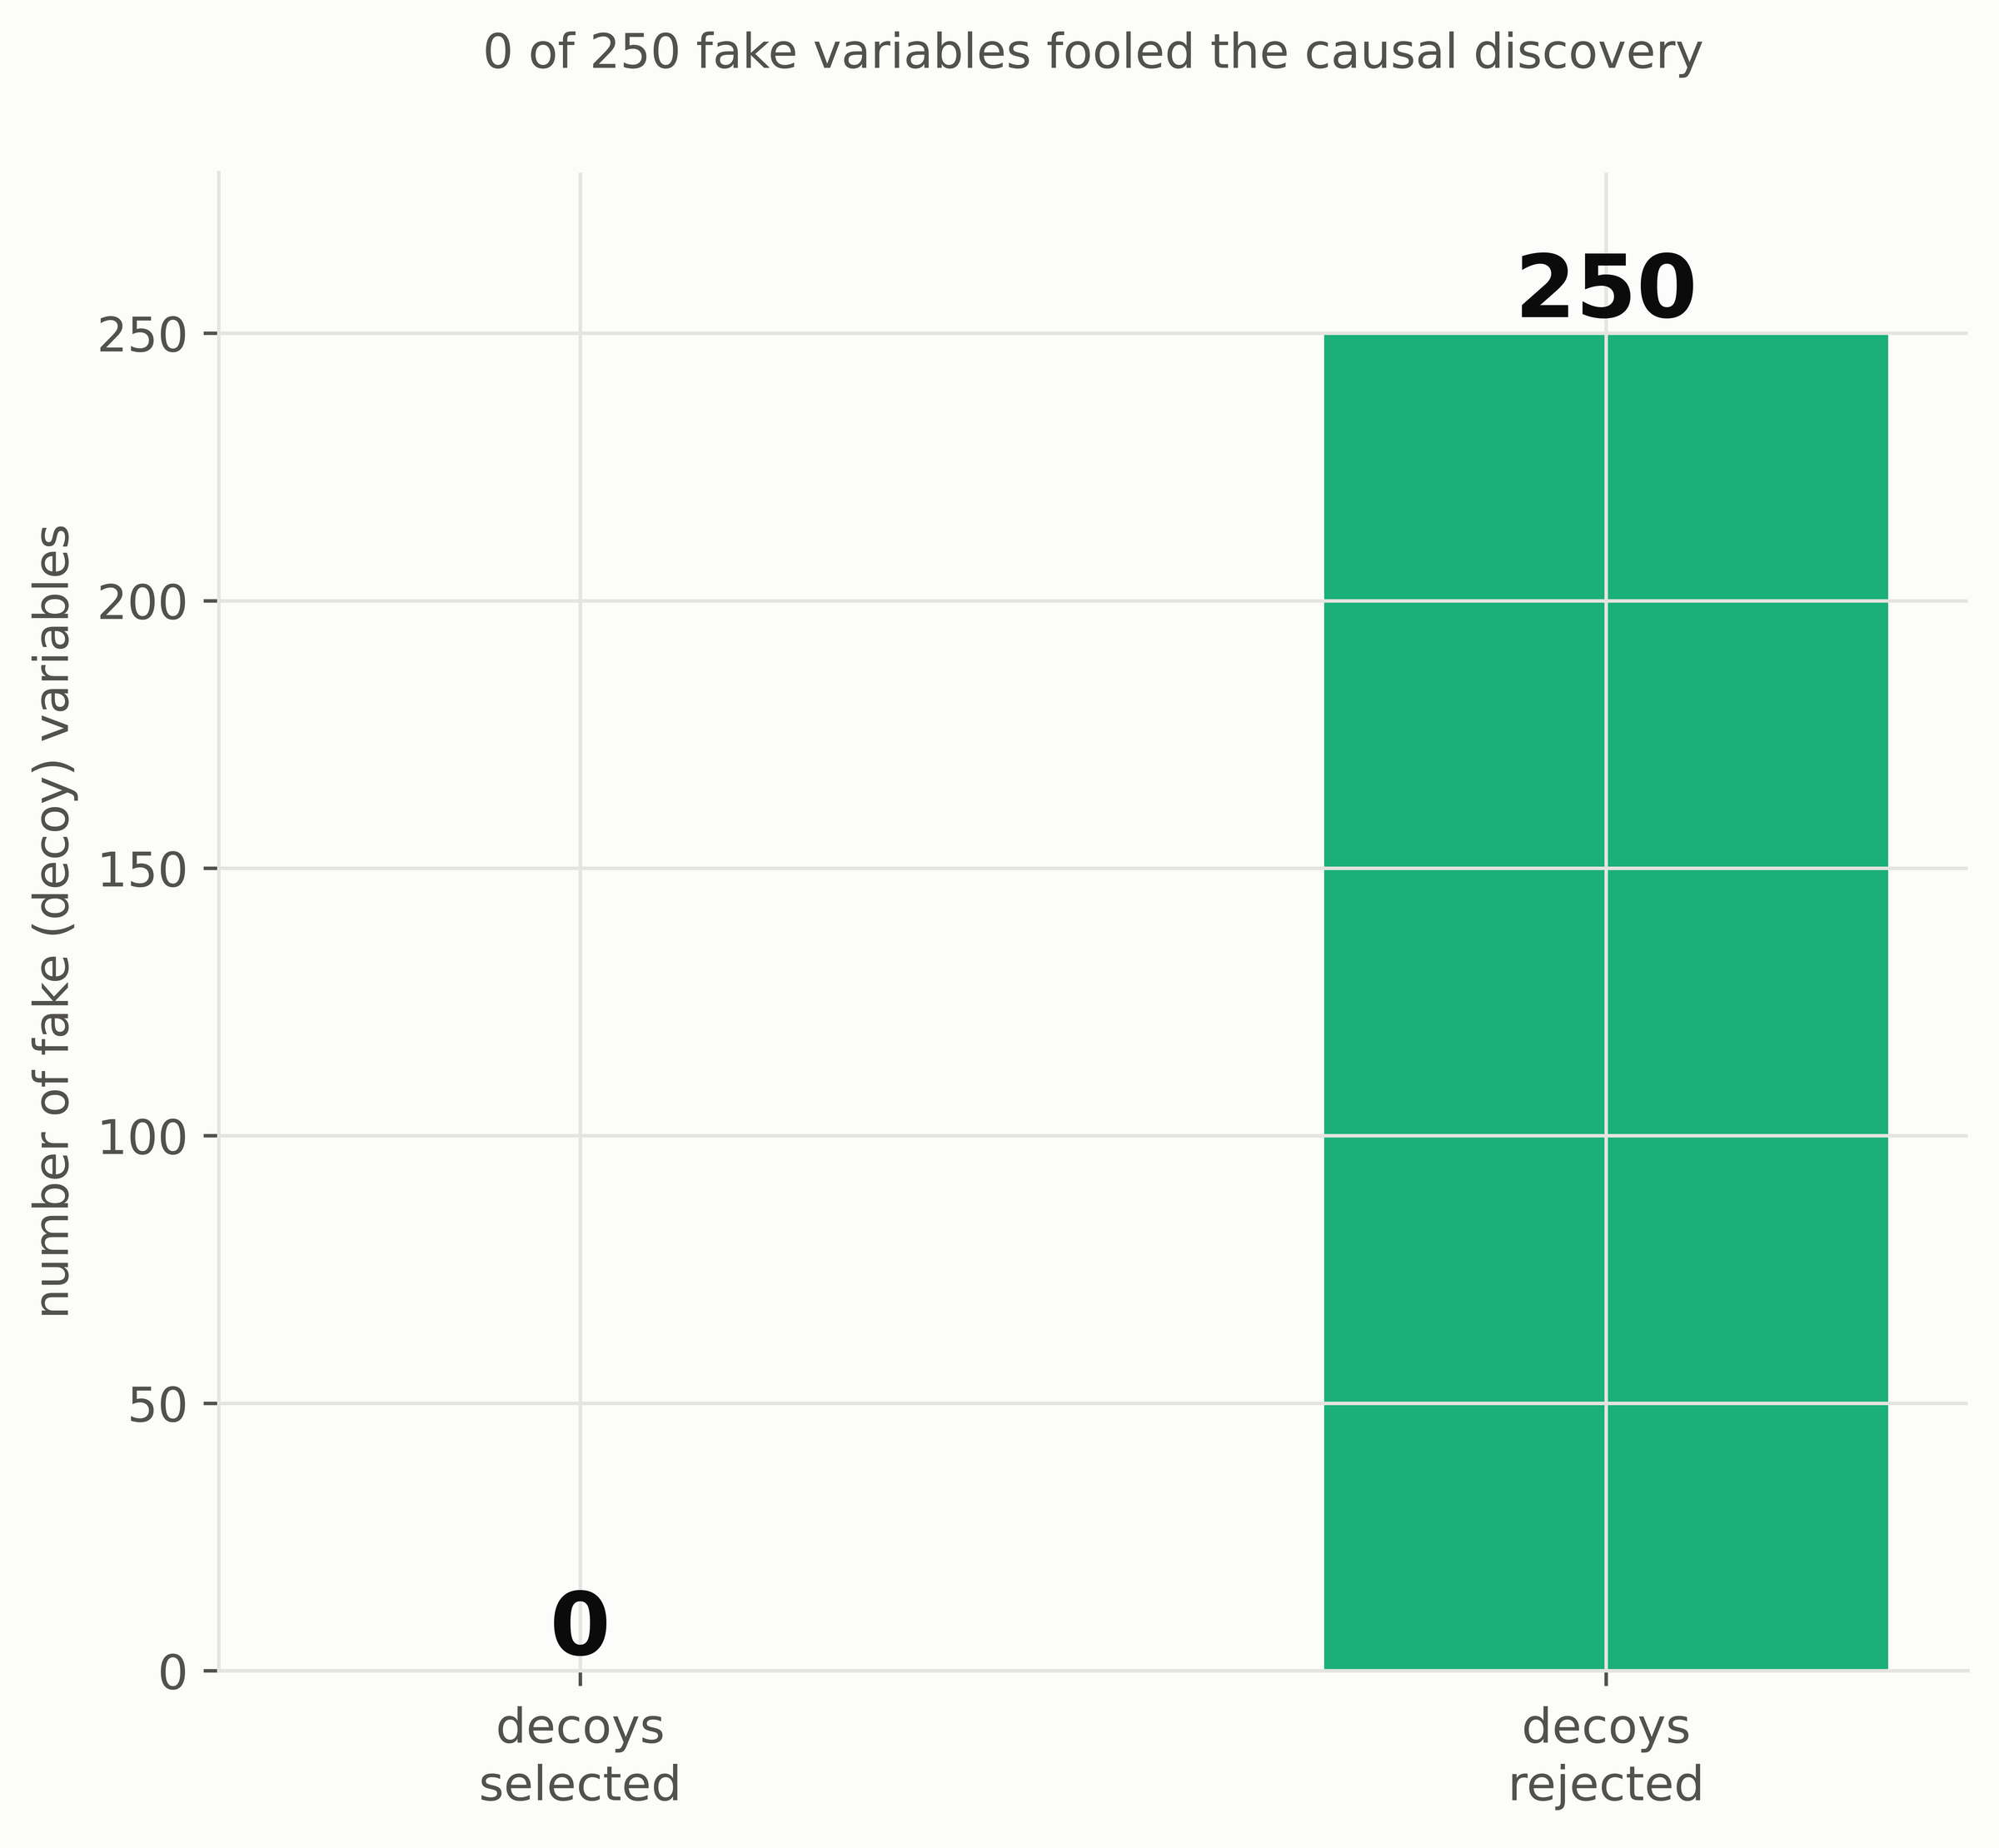
\includegraphics[width=\textwidth]{ppt_decoy_v1_big_count_bars.png}
\caption{B1: decoys selected vs rejected.}\label{fig:b1}
\end{subfigure}
\caption{The graph survives the first two checks almost unchanged. (a) Own-region links (blue) and outside links (orange) after each check. (b) None of the 250 phase-randomised decoys was selected as a parent of any target.}
\label{fig:b1b2}
\end{figure}

\paragraph{B1: decoys.} \textbf{None of the 250 decoys} was selected (decoy rate 0\%, against the 30\% warning line), while the real graph barely changed (517 real links in the decoy pass versus 536). The pipeline does not select series merely because they share the autocorrelation and the 30--60-day spectral peak of real climate nodes (Figures~\ref{fig:b1b2} and~\ref{fig:b1strength}).

\begin{figure}[htbp]
\centering
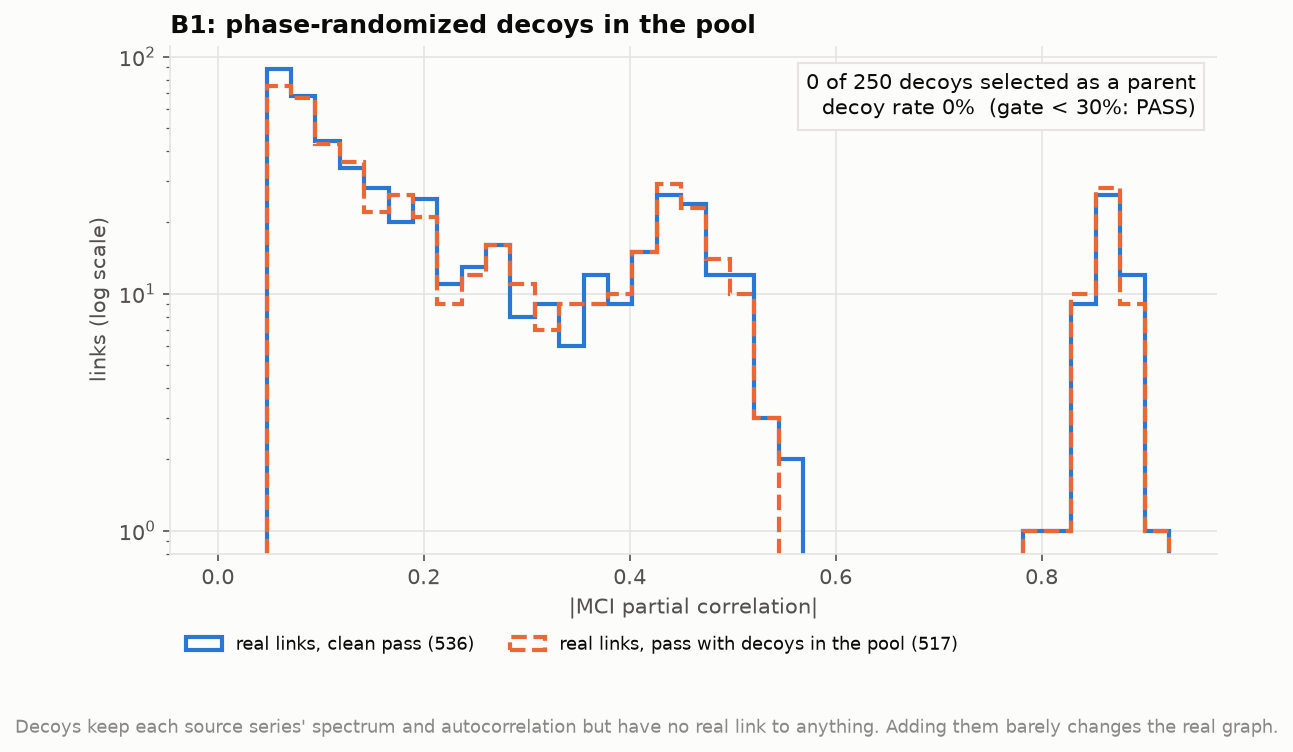
\includegraphics[width=0.7\textwidth]{04_b1_decoys.png}
\caption{B1: distribution of $|\hat\rho^{\,\mathrm{MCI}}|$ for real links in the clean pass (536) and in the pass with 250 decoys in the pool (517). The two distributions nearly coincide, including the strong own-OLR links near 0.85.}
\label{fig:b1strength}
\end{figure}

\paragraph{B2: physical lag mask.} Only \textbf{3 of 536} links need an impossible speed: h850 from region 22 to region 32 (5{,}531\,km at lag 1, 64\ms), and OLR from 28 to 33 (33\ms) and from 3 to 47 (26\ms). Of the outside links kept, 28 span 500--5{,}500\,km, and the fastest needs 46\ms; all of these come from wind and height fields, consistent with equatorial waves (Figure~\ref{fig:b2}). No link reaches the 25-day oscillation flag.

\begin{figure}[htbp]
\centering
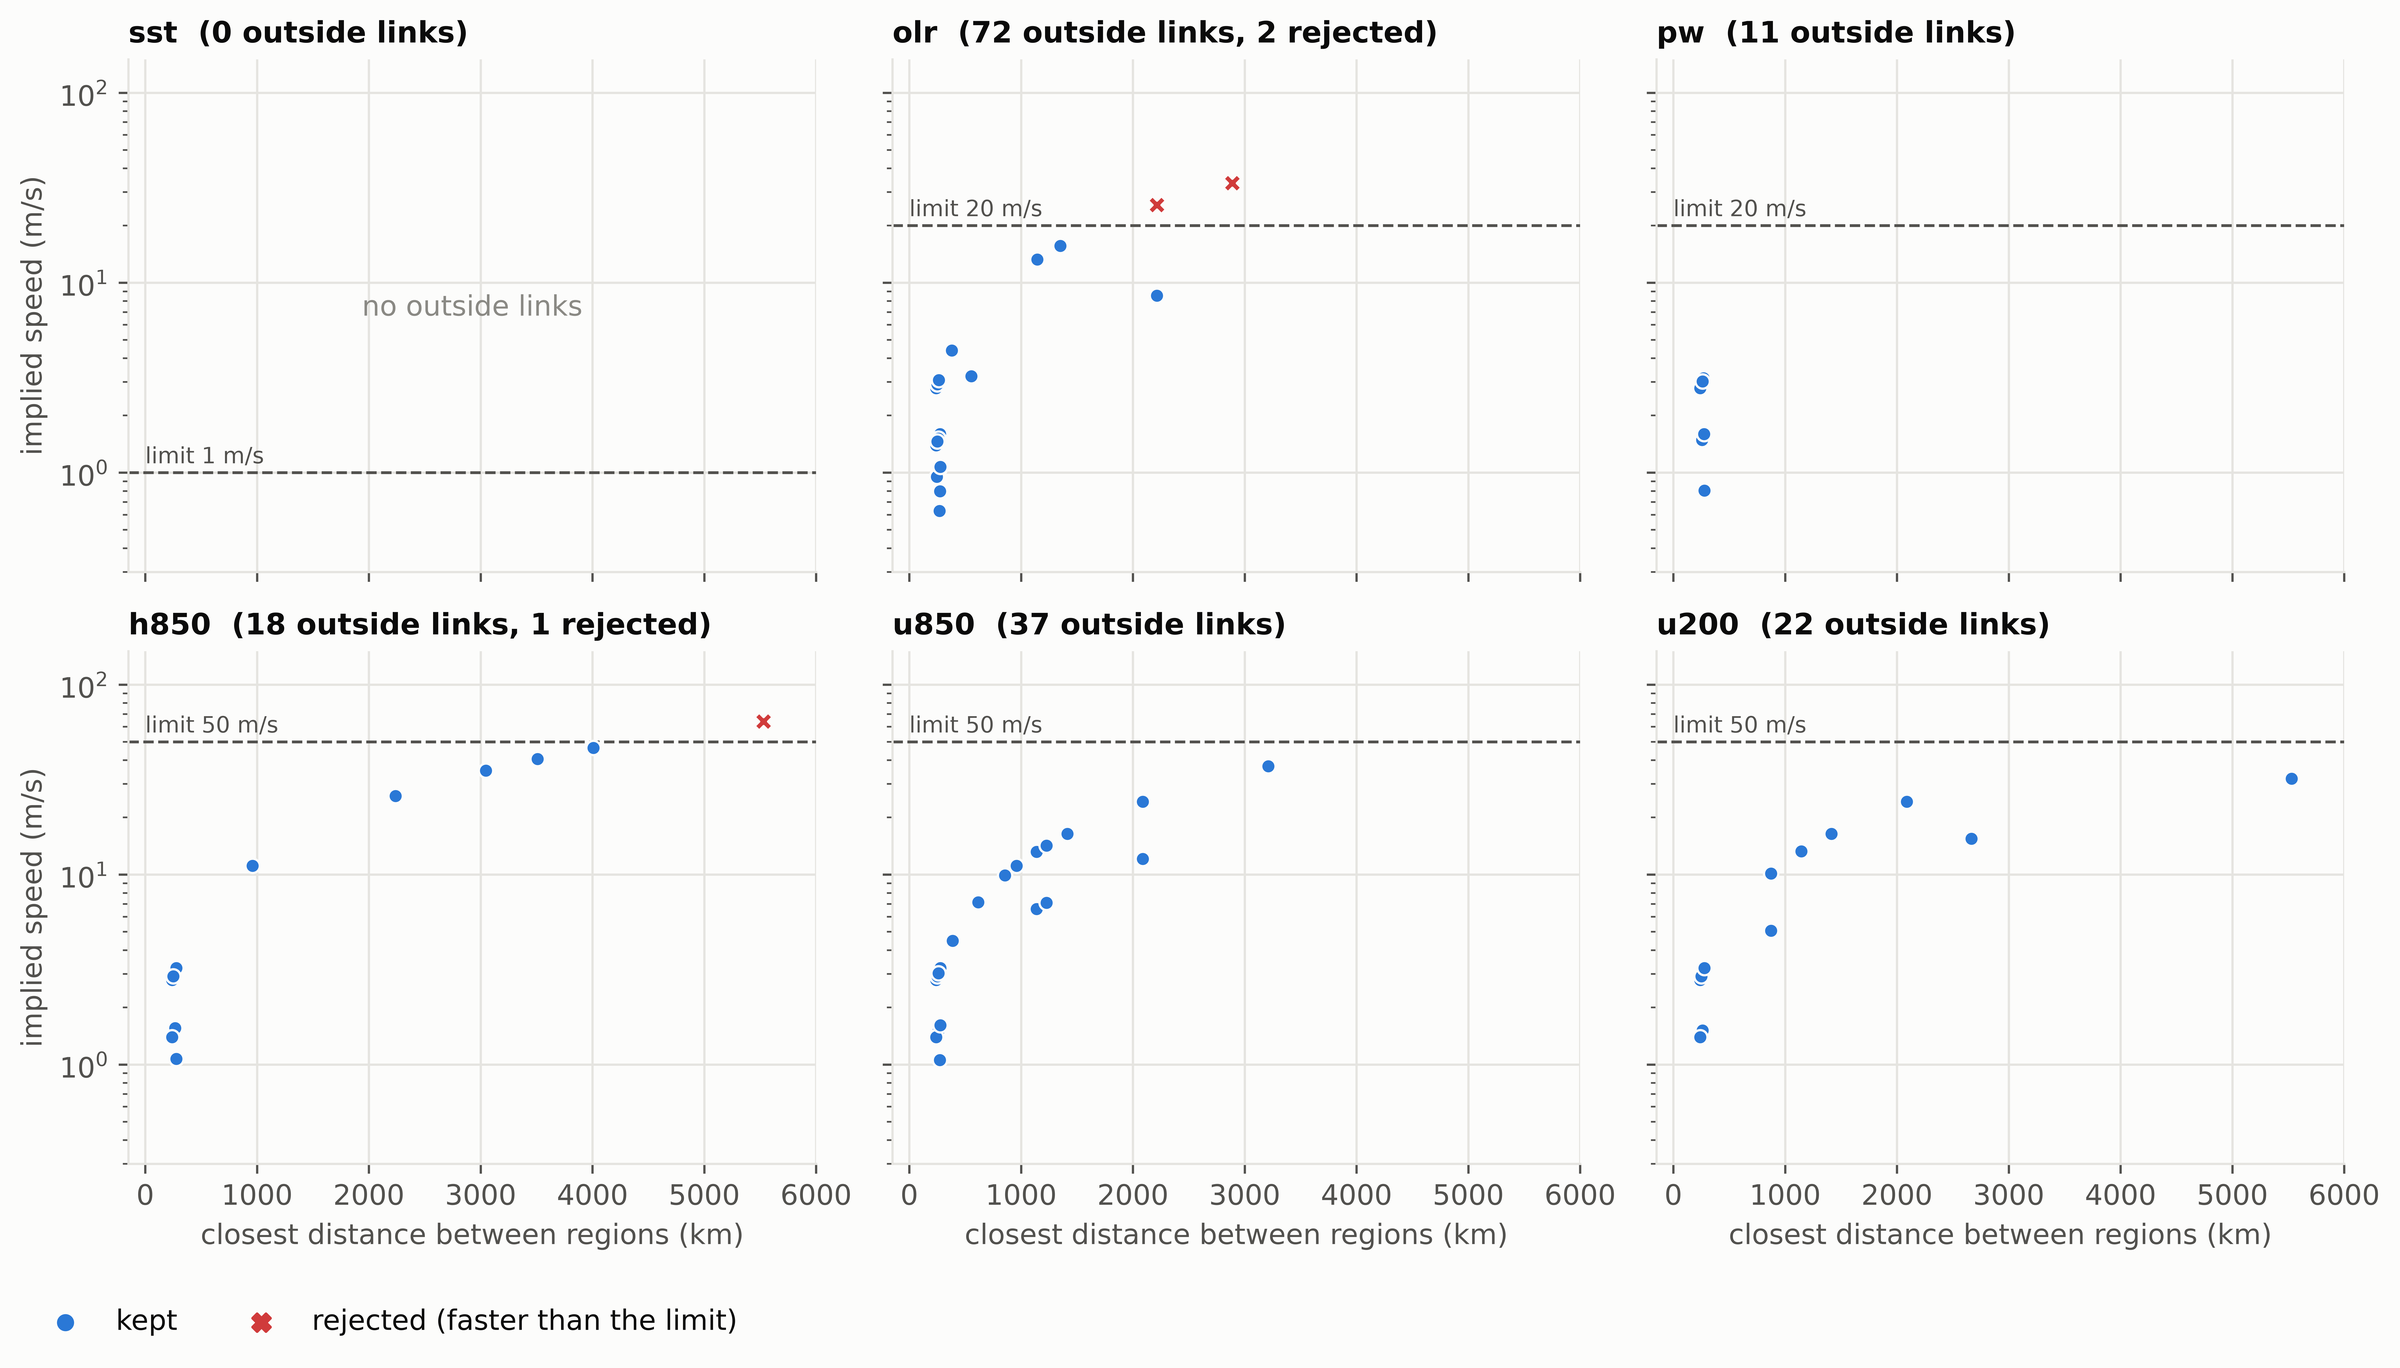
\includegraphics[width=\textwidth]{ppt_05b_b2_speed_no_title.png}
\caption{B2: implied speed against closest distance for every outside link, by source field, with each field's speed limit (dashed). Crosses are the three rejected links.}
\label{fig:b2}
\end{figure}

\paragraph{B3: top-$k$.} The validation $R^2$ rises from 0.9619 with own-region links only to 0.9633 with ten outside links, each extra link adding a little. The selected $k=10$ equals the largest number of outside links of any target, so all 157 surviving outside links are kept: PCMCI with FDR control is already sparse. The prior has \textbf{2.06 source regions per target}; two targets (regions 13 and 42) have no outside driver (Figure~\ref{fig:b3}).

\begin{figure}[htbp]
\centering
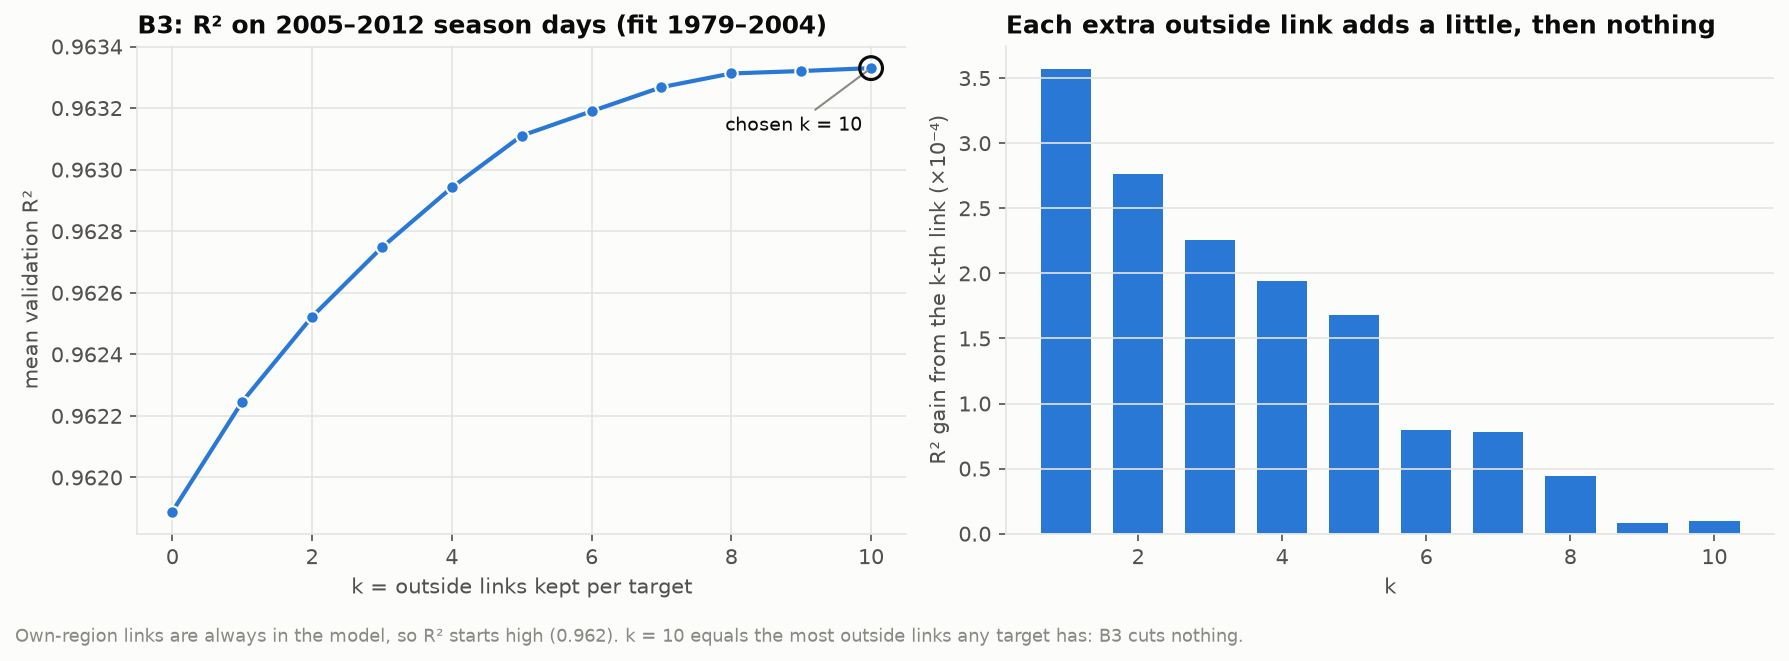
\includegraphics[width=\textwidth]{06_b3_k.png}
\caption{B3: mean validation $R^2$ on 2005--2012 season days against the number $k$ of outside links per target (left), and the gain from the $k$-th link (right).}
\label{fig:b3}
\end{figure}

\paragraph{B4: resolution persistence.} At 100 regions the mean persistence score is \textbf{0.62}, and \textbf{33 of 48} scored targets reach 0.5 (Figure~\ref{fig:b4}). OLR links persist best (56 of 70), followed by u200 (14 of 22); moisture and low-level height links, which are more local, persist least (PW 4 of 11, h850 6 of 17).

\begin{figure}[htbp]
\centering
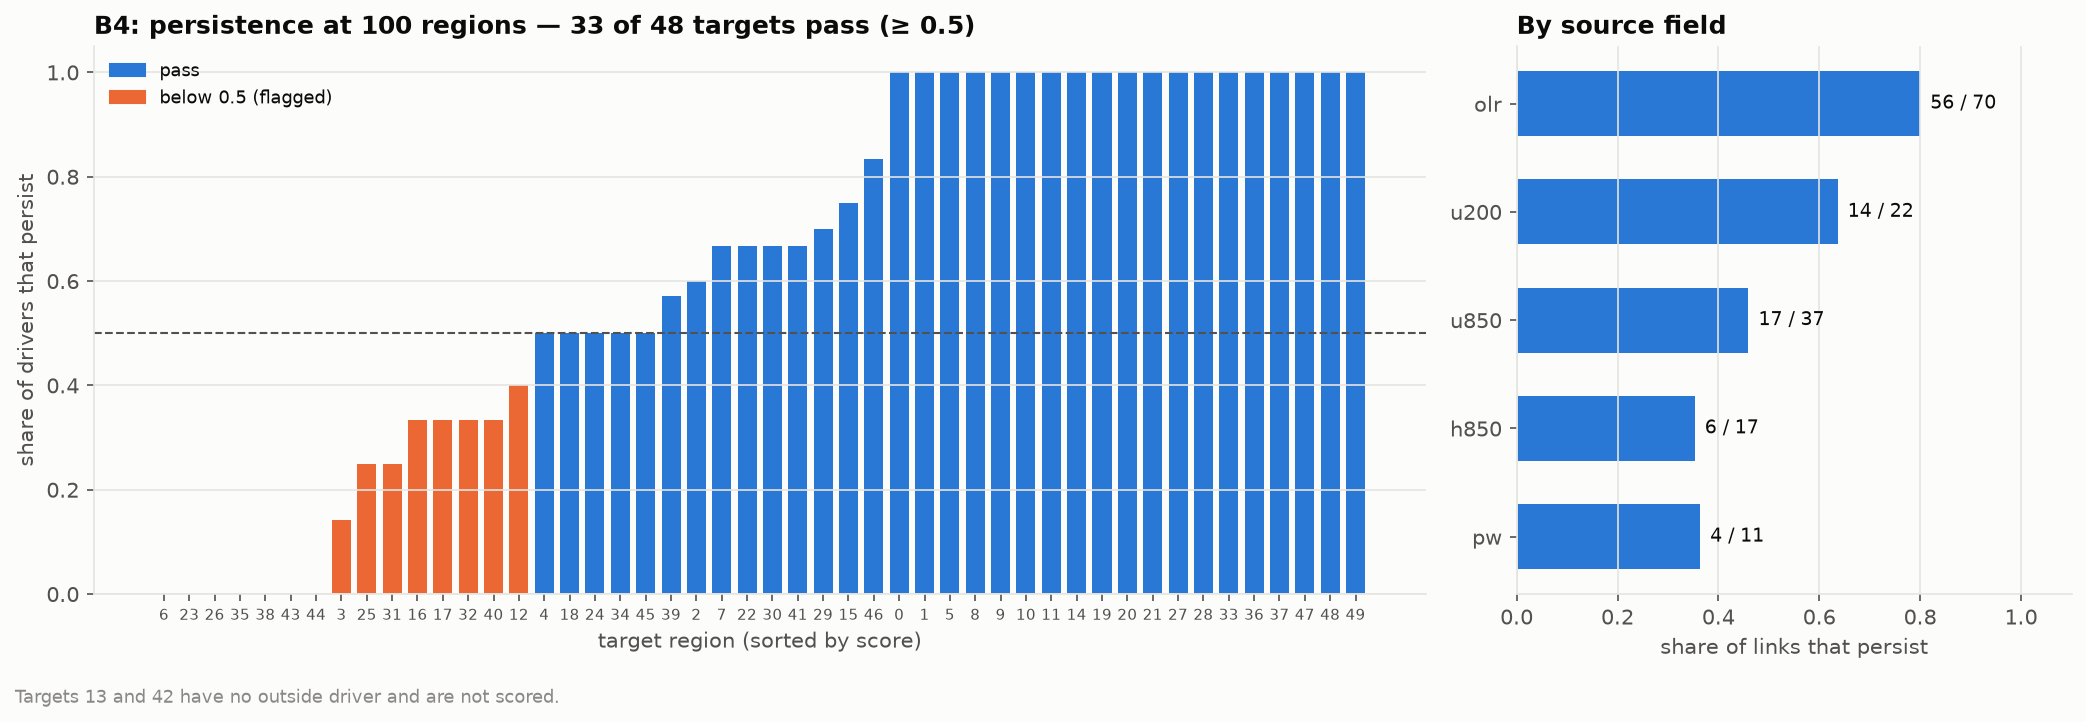
\includegraphics[width=\textwidth]{07_b4_persistence.png}
\caption{B4: persistence score of each target at 100 regions (left; orange below 0.5, flagged) and the share of links that persist by source field (right).}
\label{fig:b4}
\end{figure}

\noindent Hypotheses H1 and H2 are supported: the discovered graph is sparse, physically plausible and largely robust to the spatial partition.

\section{Source Selection and Forecasting (RQ3)}
\label{sec:res-stagec}

\subsection{The splitter without a prior}
\label{sec:res-pool}

Without a prior, the expert beats persistence at 7 days in all 50 regions in every candidate pool, with a mean skill of about $+0.40$. The year-round 7-day forecast in the direct pool has a mean MSE of 0.317 and a mean RMSE of 0.559 standard deviations (Figure~\ref{fig:mse}). Source discrimination, however, depends strongly on the pool (Table~\ref{tab:pool}): 27--30 regions have informative splitters in the direct pool, 8--9 in the 2hop pool, and none in the full pool. With 50 similar-looking candidates, the shared scoring network cannot separate them. Figure~\ref{fig:poolfig} shows the same contrast: accuracy is flat across pools while discrimination collapses. Discrimination also needs enough training: with the direct pool, 5 epochs give 27 informative regions against 5 after 2 epochs (Figure~\ref{fig:epochs}).

\begin{table}[htbp]
\centering
\caption{No-prior splitter by candidate pool, 7-day lead, 50 regions, test period 2013--2022.}
\label{tab:pool}
\footnotesize
\setlength{\tabcolsep}{3pt}
\begin{tabular}{llccc}
\toprule
\textbf{Target days} & \textbf{Pool} & \textbf{Informative splitters} & \textbf{Beat persistence} & \textbf{Mean $S_{\mathrm{pers}}$} \\
\midrule
Year-round & direct / 2hop / full & 27 / 8 / 0 & 50 / 50 / 50 & $+0.401$ / $+0.395$ / $+0.396$ \\
BSISO season & direct / 2hop / full & 30 / 9 / 0 & 50 / 50 / 50 & $+0.412$ / $+0.413$ / $+0.415$ \\
\bottomrule
\end{tabular}
\end{table}

\begin{figure}[htbp]
\centering
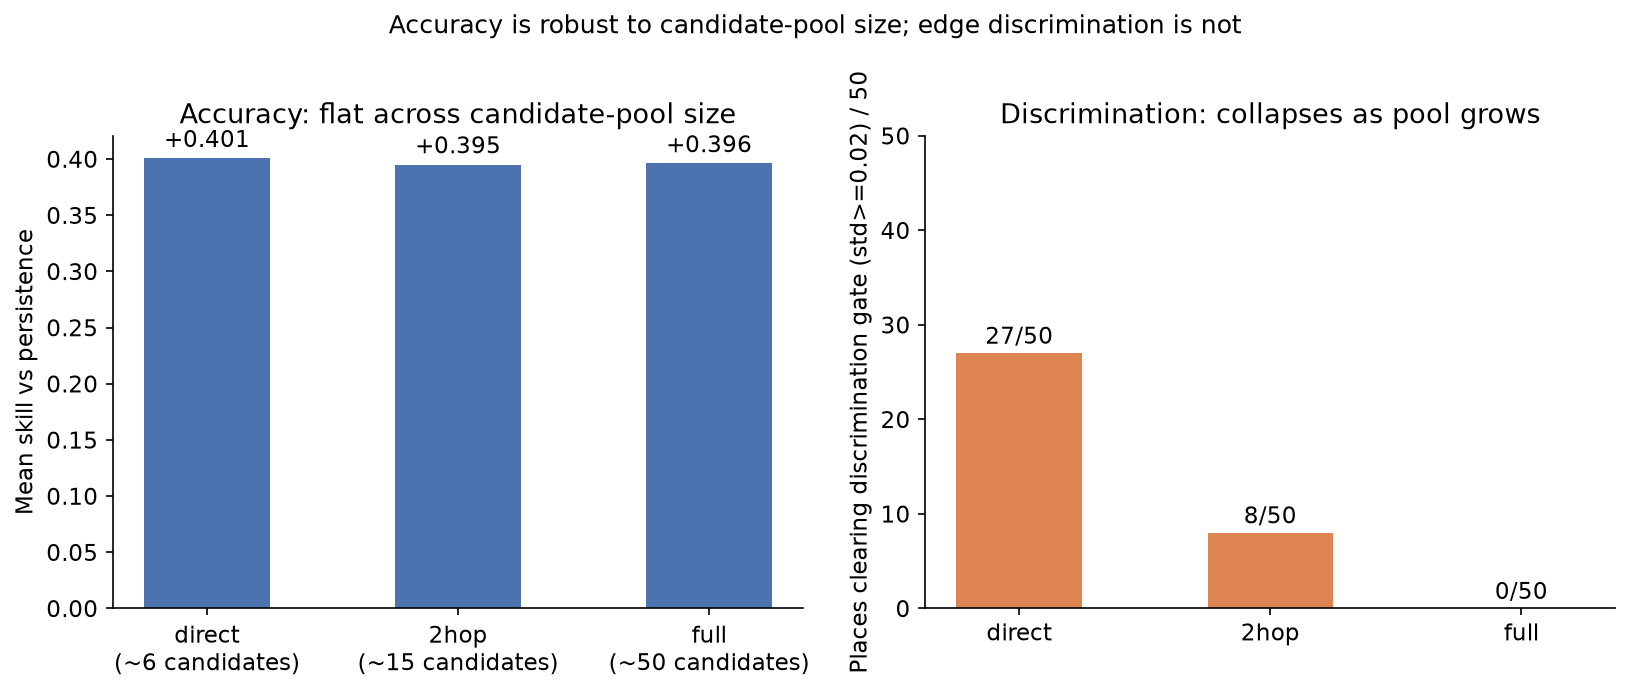
\includegraphics[width=0.85\textwidth]{02_variant_comparison.png}
\caption{No-prior splitter, year-round, 7-day lead: skill relative to persistence is flat across candidate pools (left), while the number of regions with informative splitter scores collapses as the pool grows (right).}
\label{fig:poolfig}
\end{figure}

\begin{figure}[htbp]
\centering
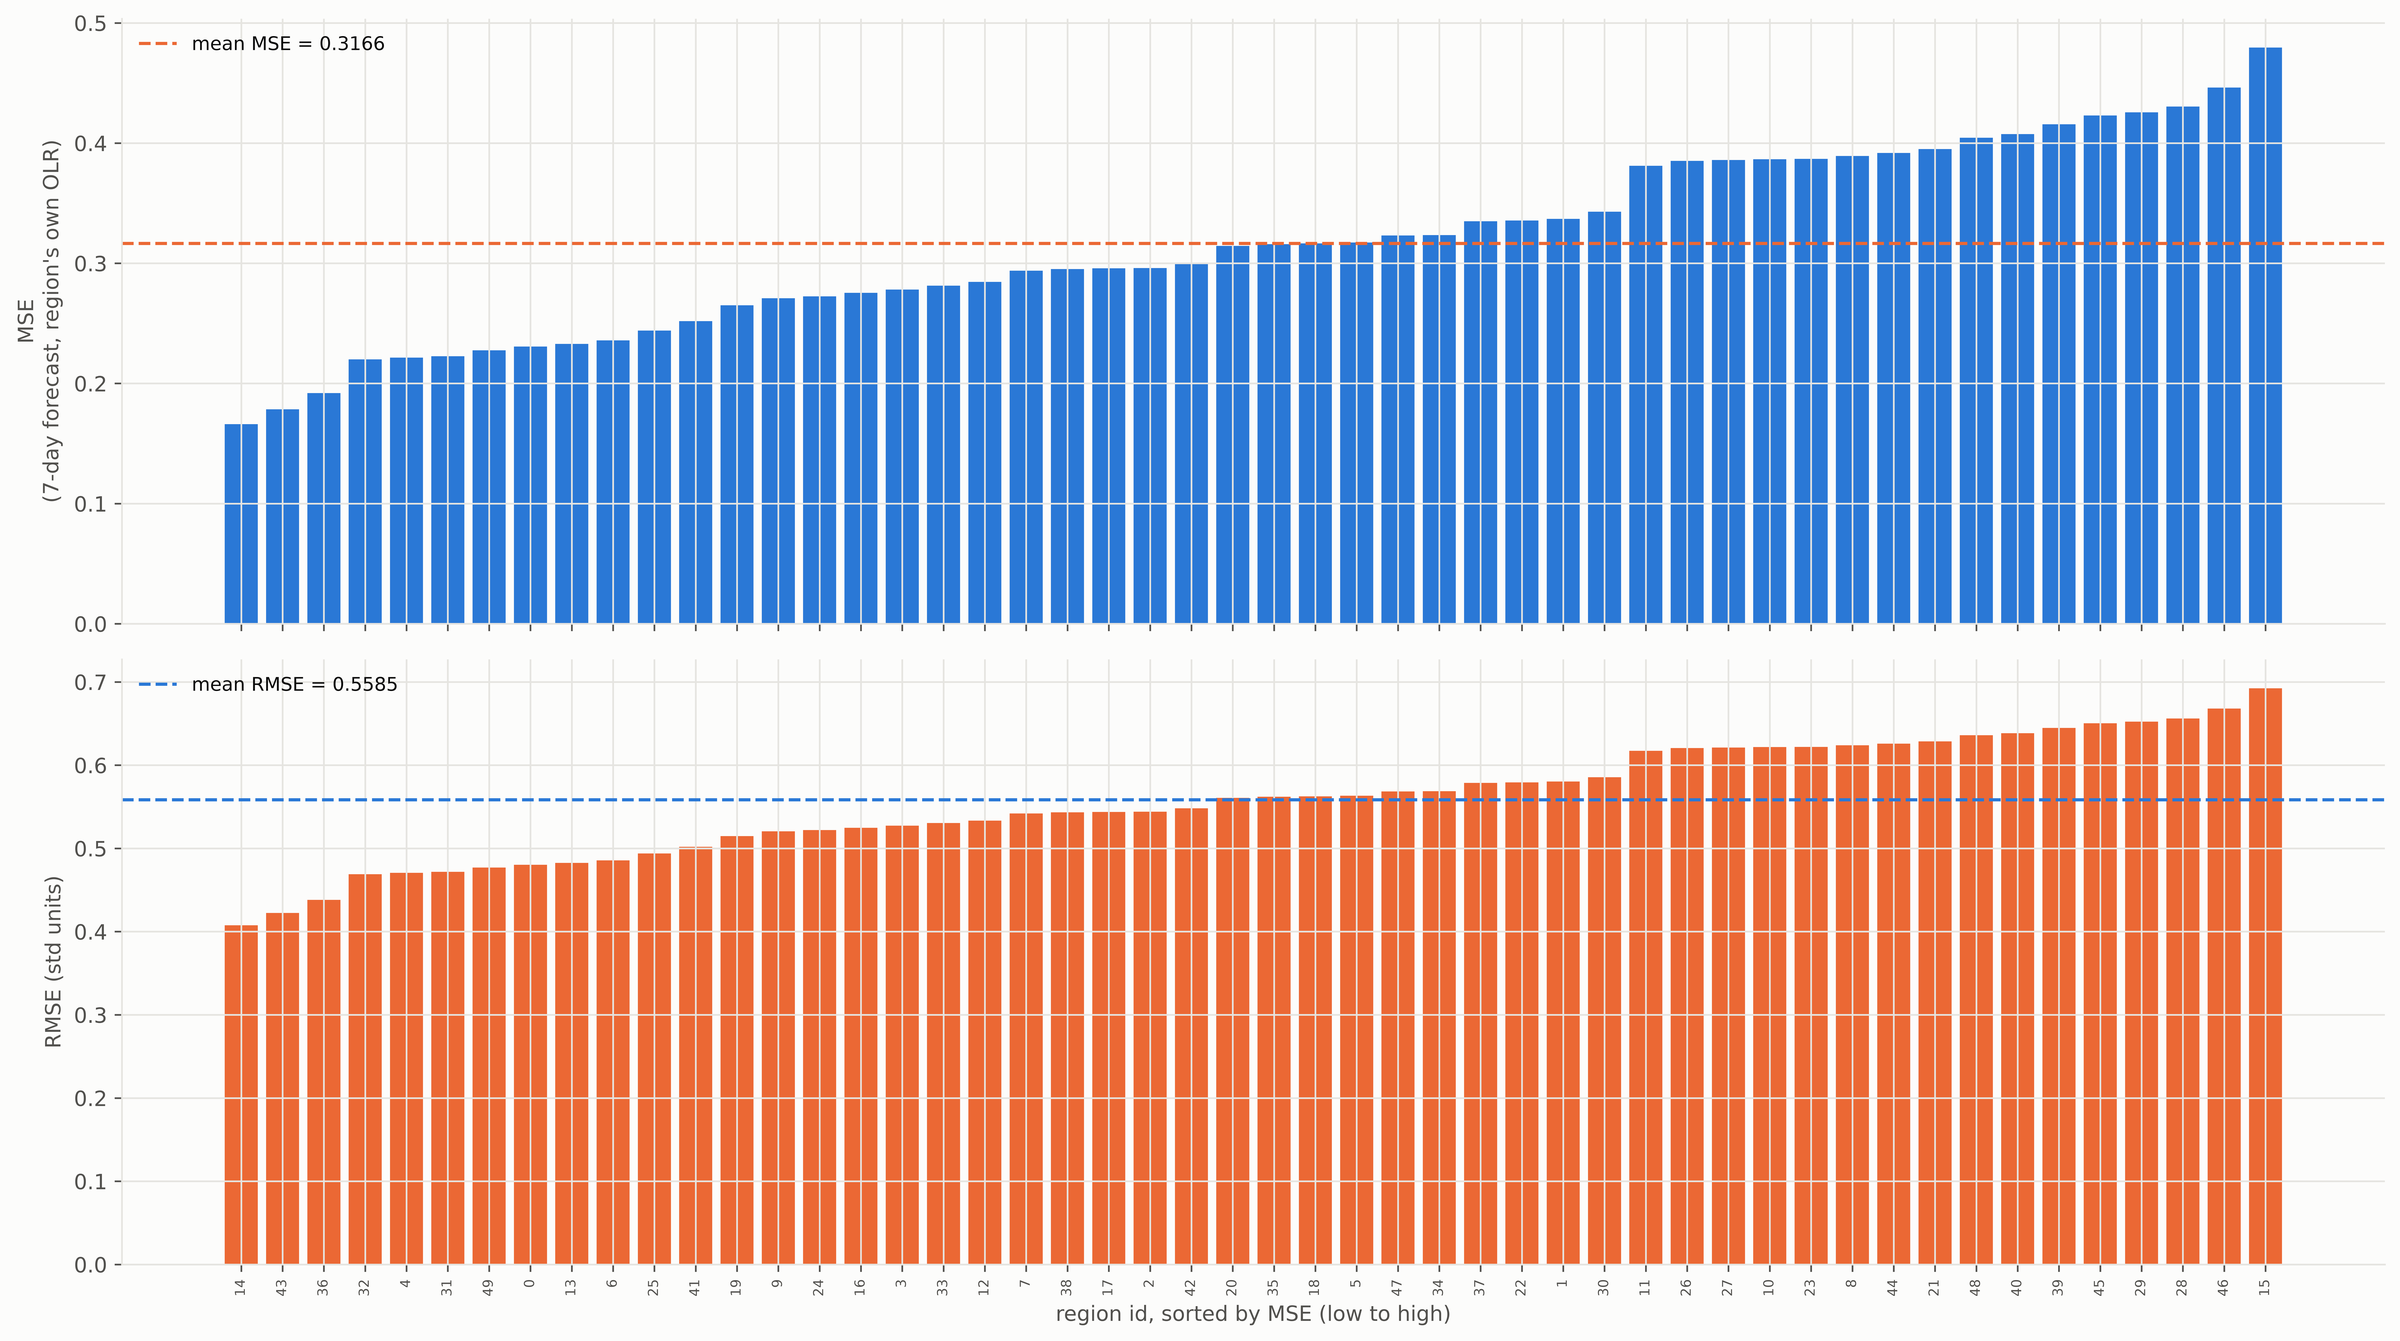
\includegraphics[width=\textwidth]{ppt_c3_per_region_mse_rmse_7day.png}
\caption{Per-region MSE (top) and RMSE (bottom) of the 7-day OLR forecast, direct pool, year-round test 2013--2022, sorted by error. Dashed lines: means (MSE 0.317, RMSE 0.559).}
\label{fig:mse}
\end{figure}

\begin{figure}[htbp]
\centering
\begin{subfigure}[b]{0.38\textwidth}\centering
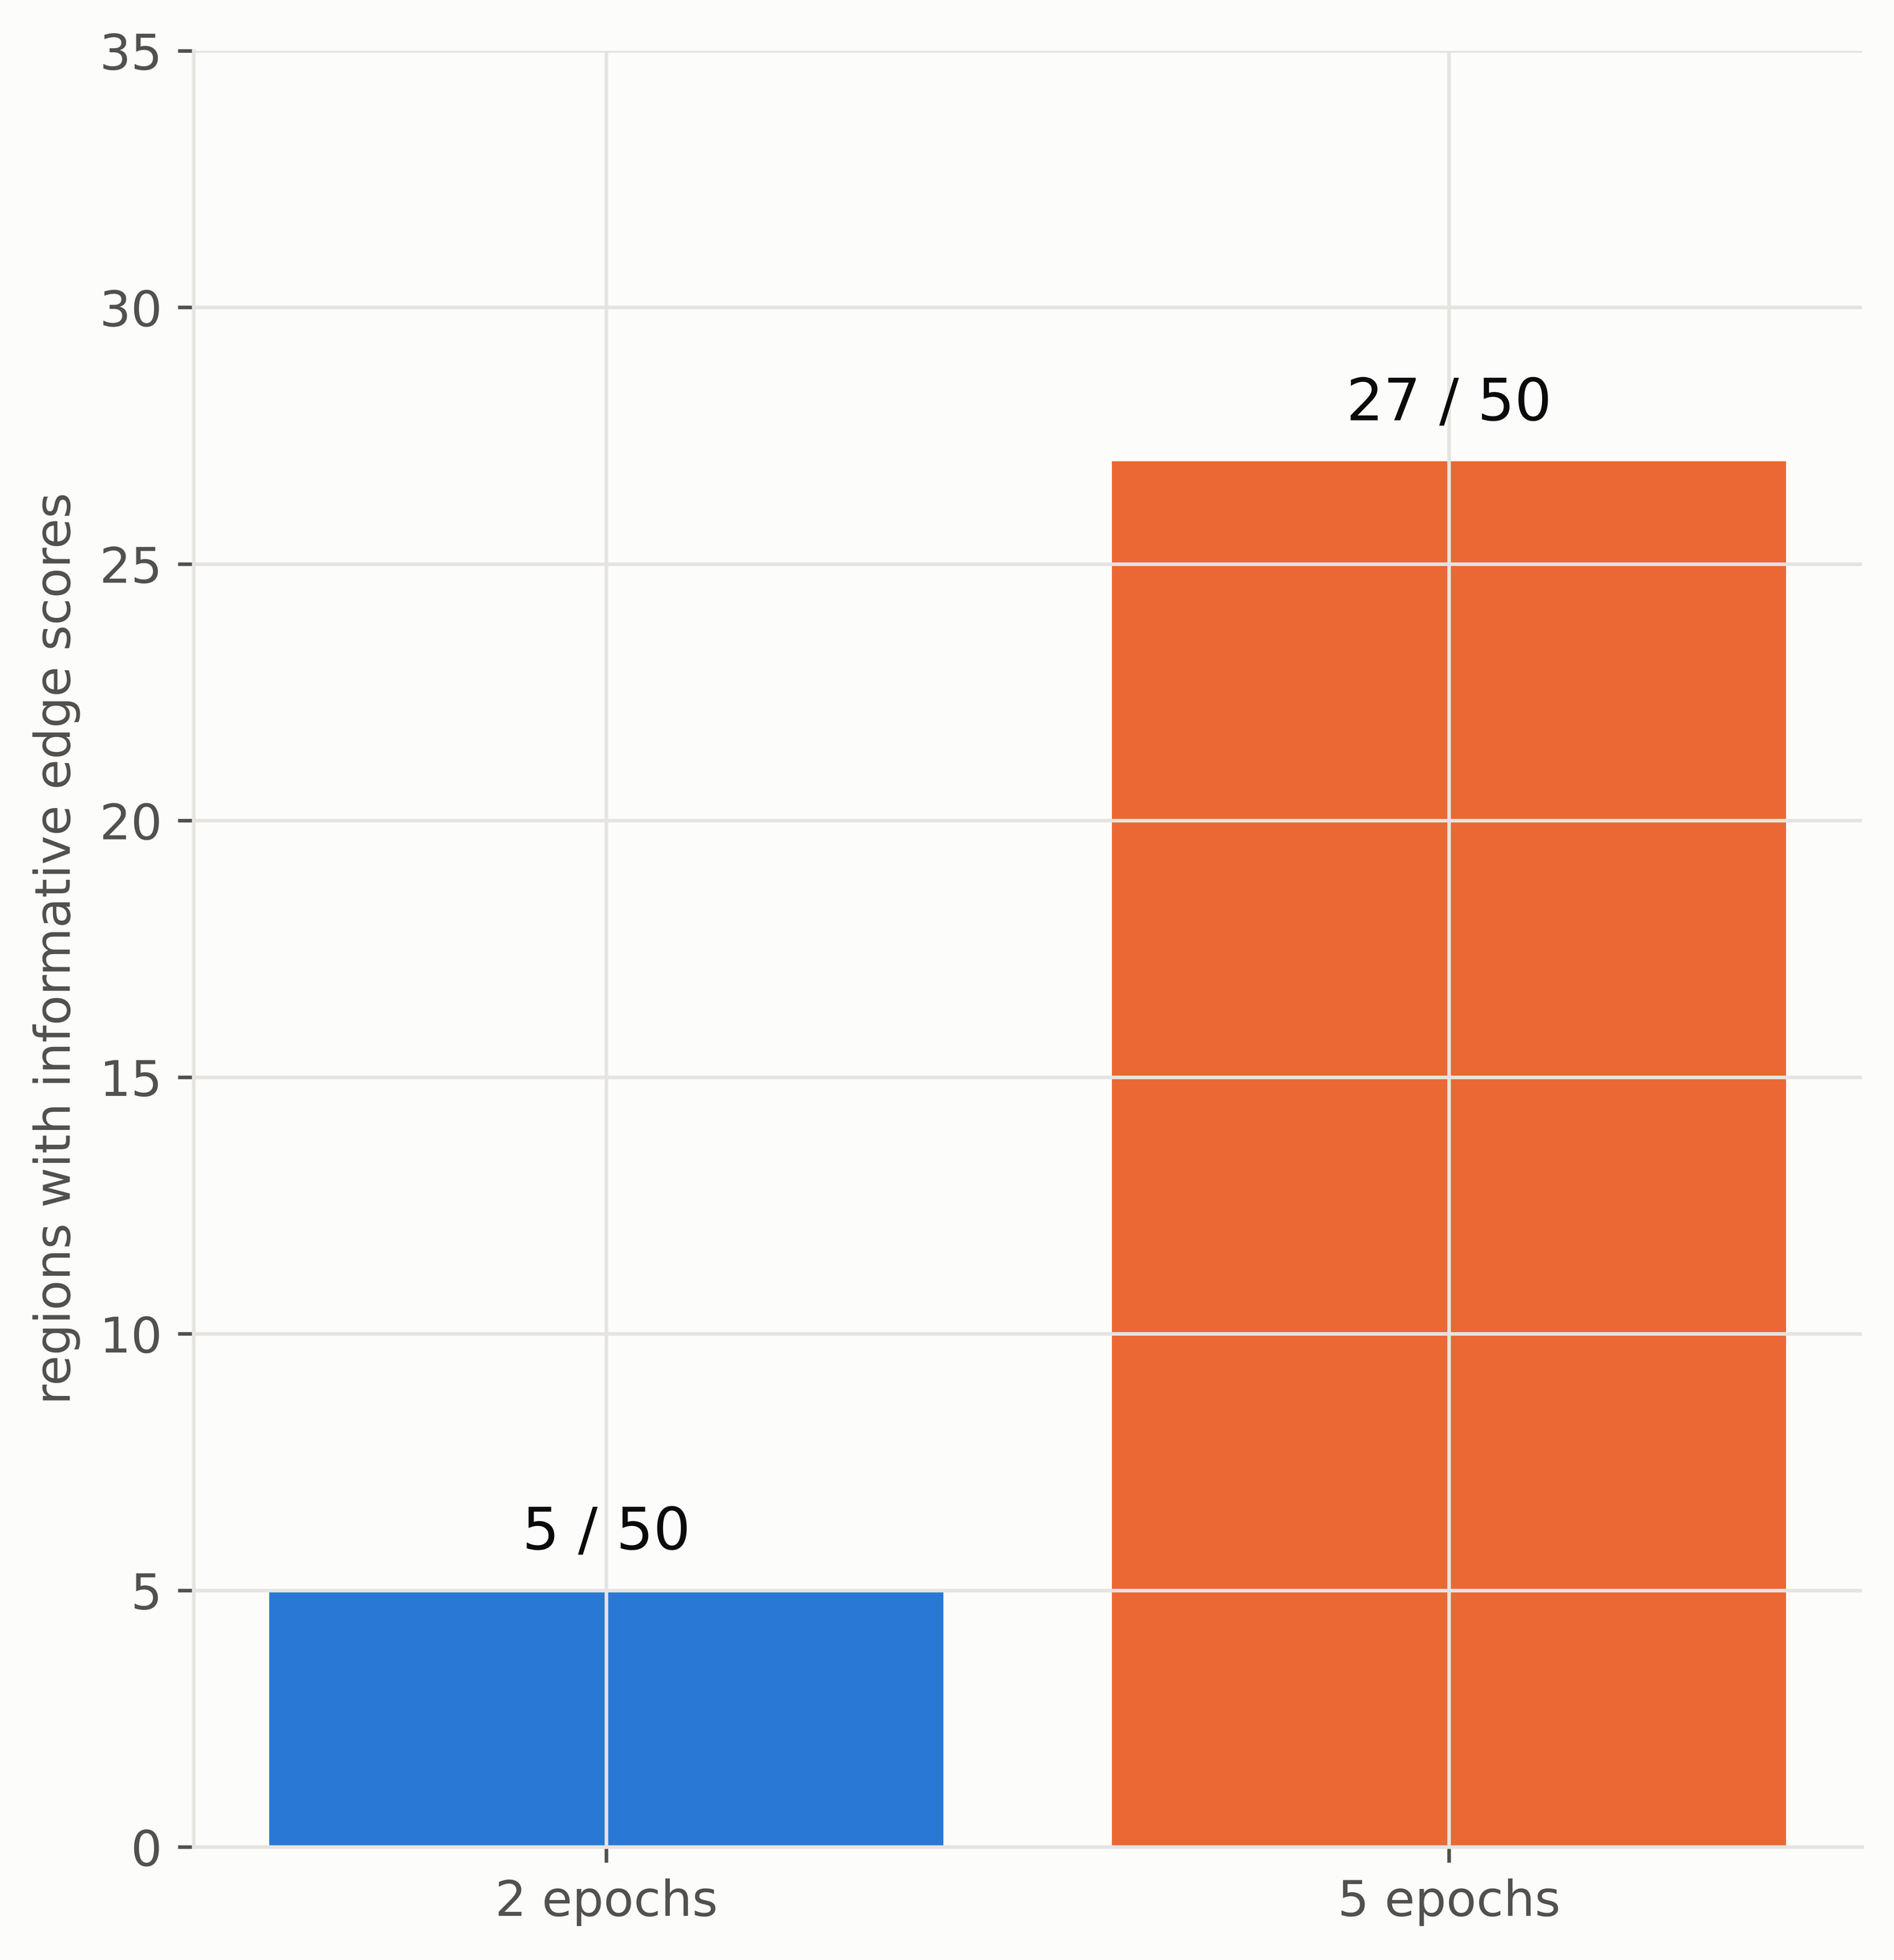
\includegraphics[width=\textwidth]{ppt_03c_informative_scores_2_vs_5_epochs.png}
\caption{Informative splitters, 2 vs 5 epochs.}\label{fig:epochs}
\end{subfigure}\hfill
\begin{subfigure}[b]{0.58\textwidth}\centering
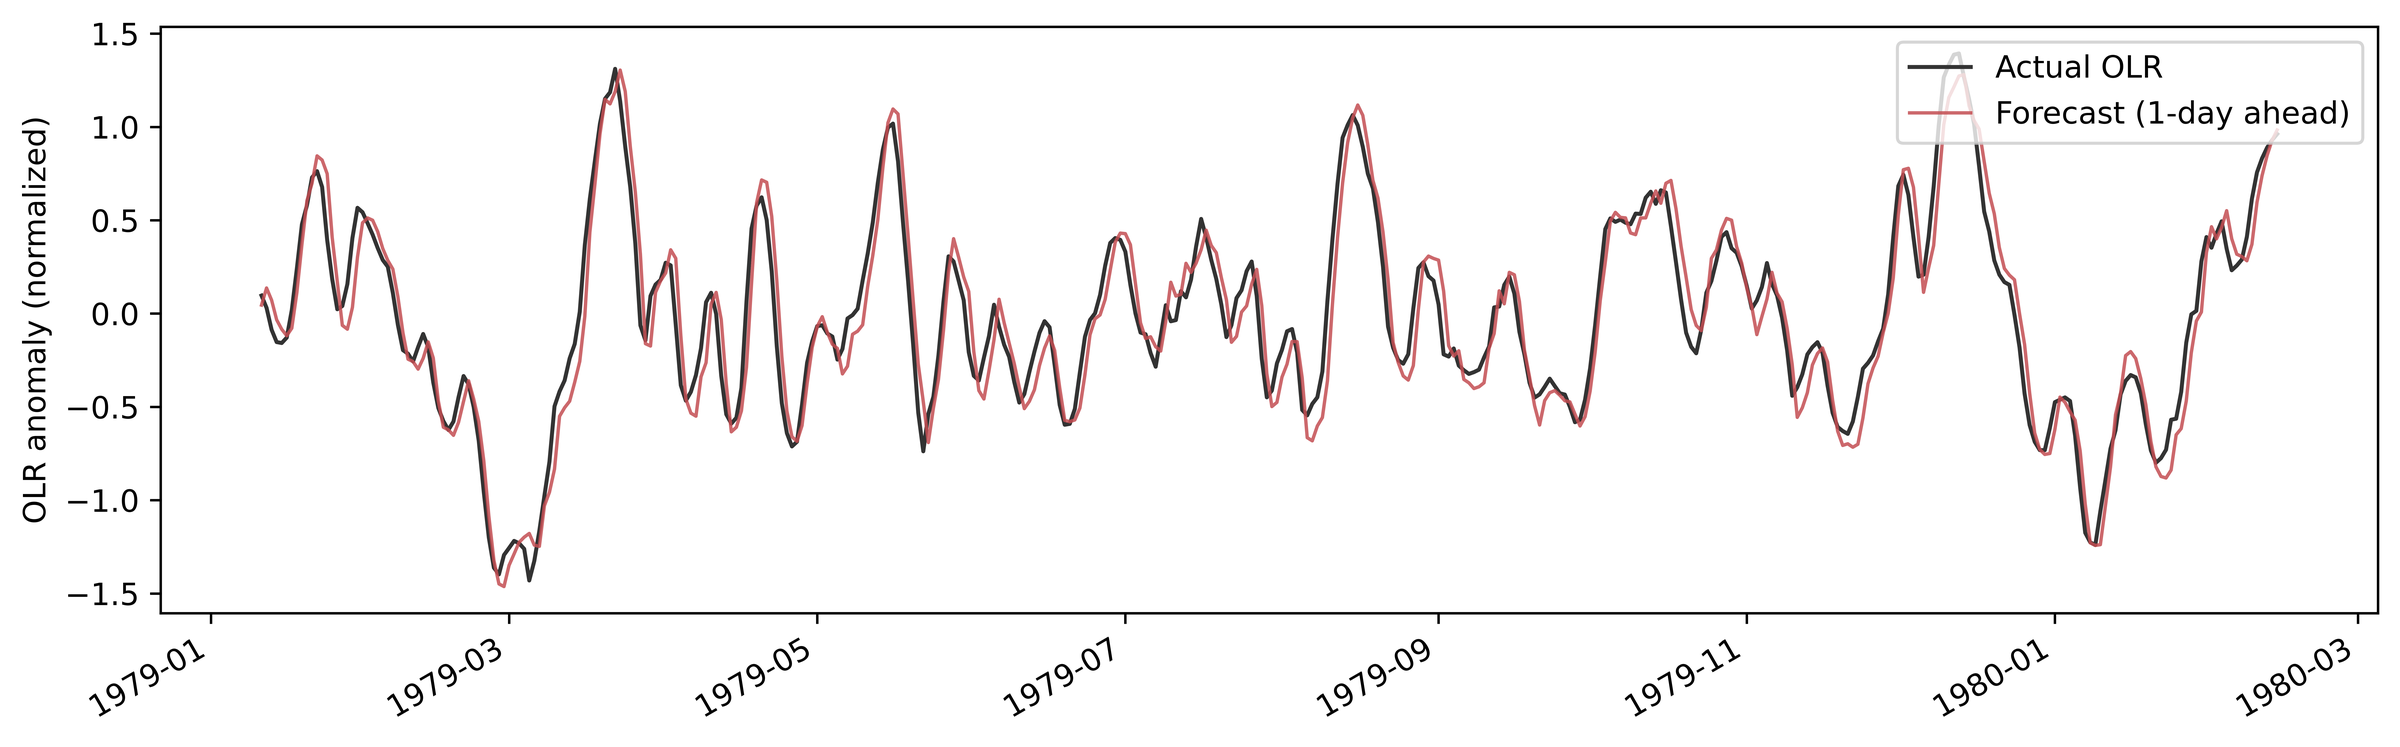
\includegraphics[width=\textwidth]{ppt_09_2_forecast_vs_actual_no_title.png}
\caption{Region 22, 1-day forecast vs observed OLR (illustrative 1979--80 window).}\label{fig:fva}
\end{subfigure}
\caption{(a) Splitter discrimination needs an adequate training budget. (b) The expert follows the observed OLR anomalies one day ahead, including sharp swings; held-out scores are reported in Table~\ref{tab:stagec}.}
\label{fig:epochs-fva}
\end{figure}

\subsection{The causal graph as a prior}

Table~\ref{tab:stagec} compares the PCMCI prior in restrict mode with no prior in the full pool on the 1{,}989 held-out season days.

\begin{table}[htbp]
\centering
\caption{PCMCI prior (restrict) vs no prior, full 50-region pool, 2013--2022 season days.}
\label{tab:stagec}
\footnotesize
\begin{tabular}{llccccc}
\toprule
\textbf{Lead} & \textbf{Prior} & \textbf{Informative} & \textbf{Beat pers.} & \textbf{Mean $S_{\mathrm{pers}}$} & \textbf{Beat clim.} & \textbf{Mean $R^2_{\mathrm{clim}}$} \\
\midrule
7 days & none & 0/50 & 50/50 & $+0.415$ & 14/50 & $-0.015$ \\
 & PCMCI & \textbf{24/50} & 50/50 & $+0.416$ & \textbf{19/50} & $-0.015$ \\
\midrule
1 day & none & 0/50 & 0/50 & $-1.527$ & 50/50 & $+0.720$ \\
 & PCMCI & \textbf{36/50} & 3/50 & $\mathbf{-1.327}$ & 50/50 & $\mathbf{+0.745}$ \\
\bottomrule
\end{tabular}
\end{table}

\paragraph{The prior makes source selection informative.} In the full pool, where the unguided splitter is uninformative in every region, the restrict prior yields informative splitters in 24 regions at 7 days and 36 at 1 day, without loss of accuracy.

\paragraph{One-day lead: skill improves.} The prior improves skill in \textbf{32 of 50 regions} (Figure~\ref{fig:stagec1}), with median gains of $+0.40$ in $S_{\mathrm{pers}}$ and $+0.048$ in $R^2_{\mathrm{clim}}$ (Wilcoxon $p=0.049$) and a median 17\% reduction in MSE. Region 22 improves from $S_{\mathrm{pers}}=-0.60$ to $-0.05$. Skill against persistence is negative at one day for both models because tomorrow's OLR is very close to today's; both are clearly skilful against climatology ($R^2_{\mathrm{clim}}>0.7$).

\begin{figure}[htbp]
\centering
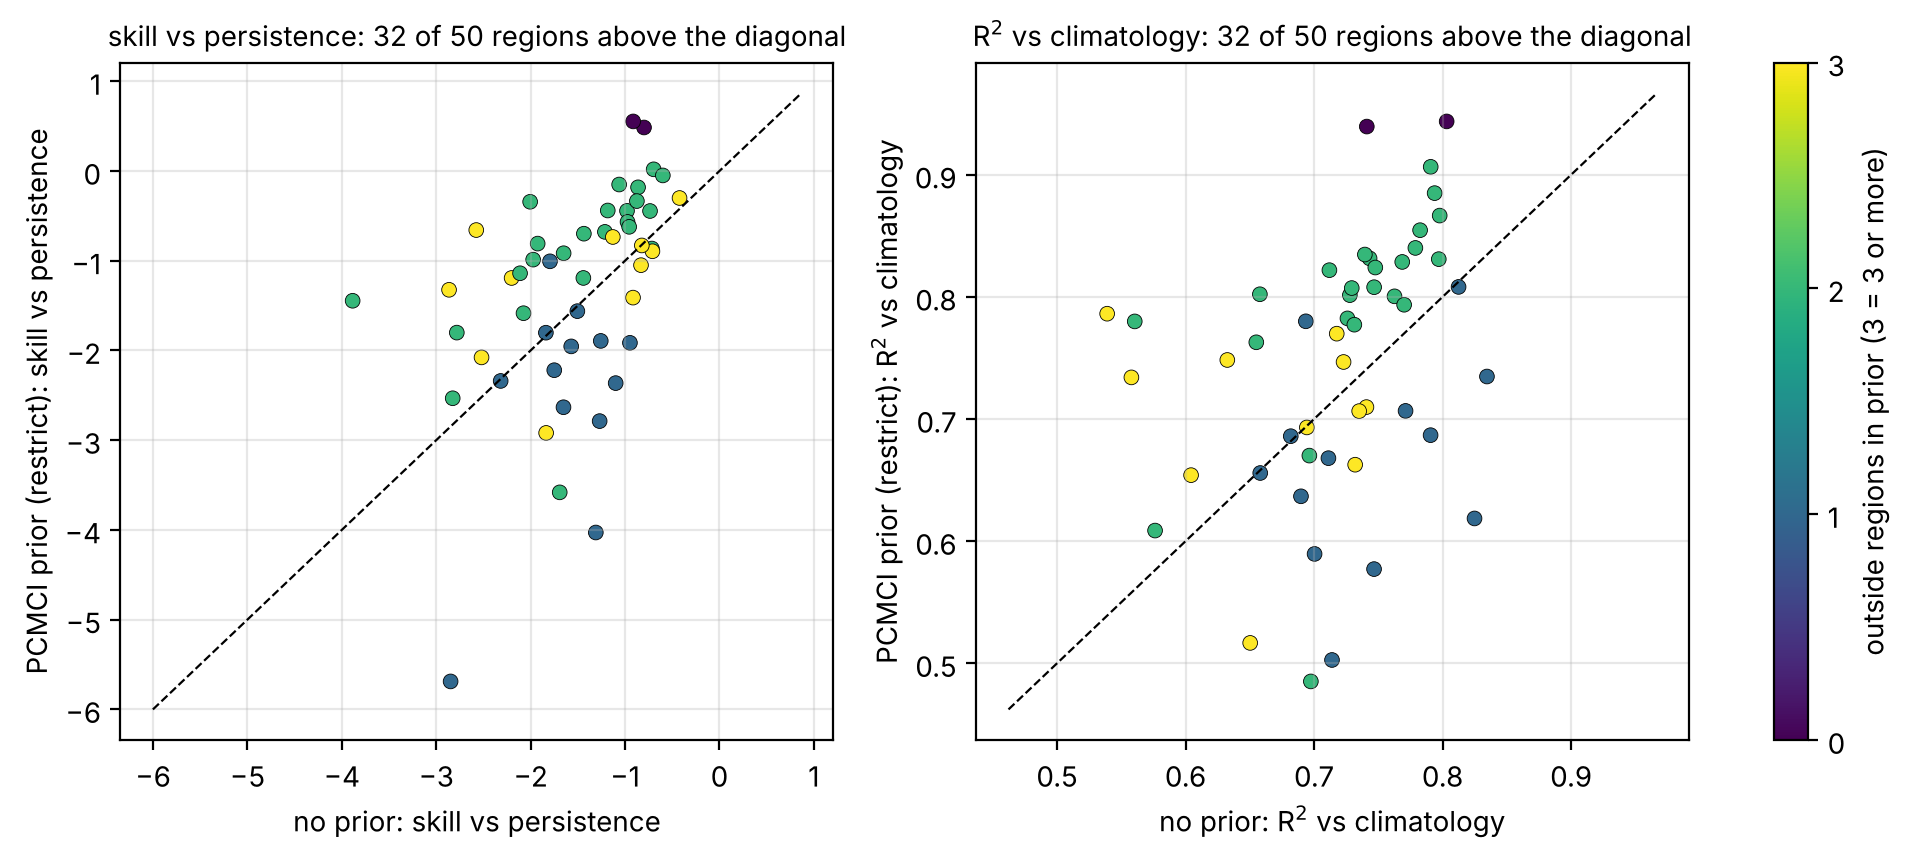
\includegraphics[width=0.92\textwidth]{10_stage_c_lead1.png}
\caption{One-day lead, full pool: per-region skill with the PCMCI prior against skill without a prior. Points above the diagonal improve; colour gives the number of outside regions in the prior.}
\label{fig:stagec1}
\end{figure}

\paragraph{Seven-day lead: unchanged.} At 7 days, skill is unchanged (23 regions better, 27 worse; mean $S_{\mathrm{pers}}$ $+0.416$ versus $+0.415$; Figure~\ref{fig:stagec7}), although 19 rather than 14 regions beat climatology. This follows from the graph's time scale: its outside links act within one or two days, so they describe exactly the information a 1-day forecast can use, but a source's state seven days before the target adds little. The graph identifies the right \emph{neighbours}, while a 7-day forecast needs week-ahead \emph{precursors}.

\begin{figure}[htbp]
\centering
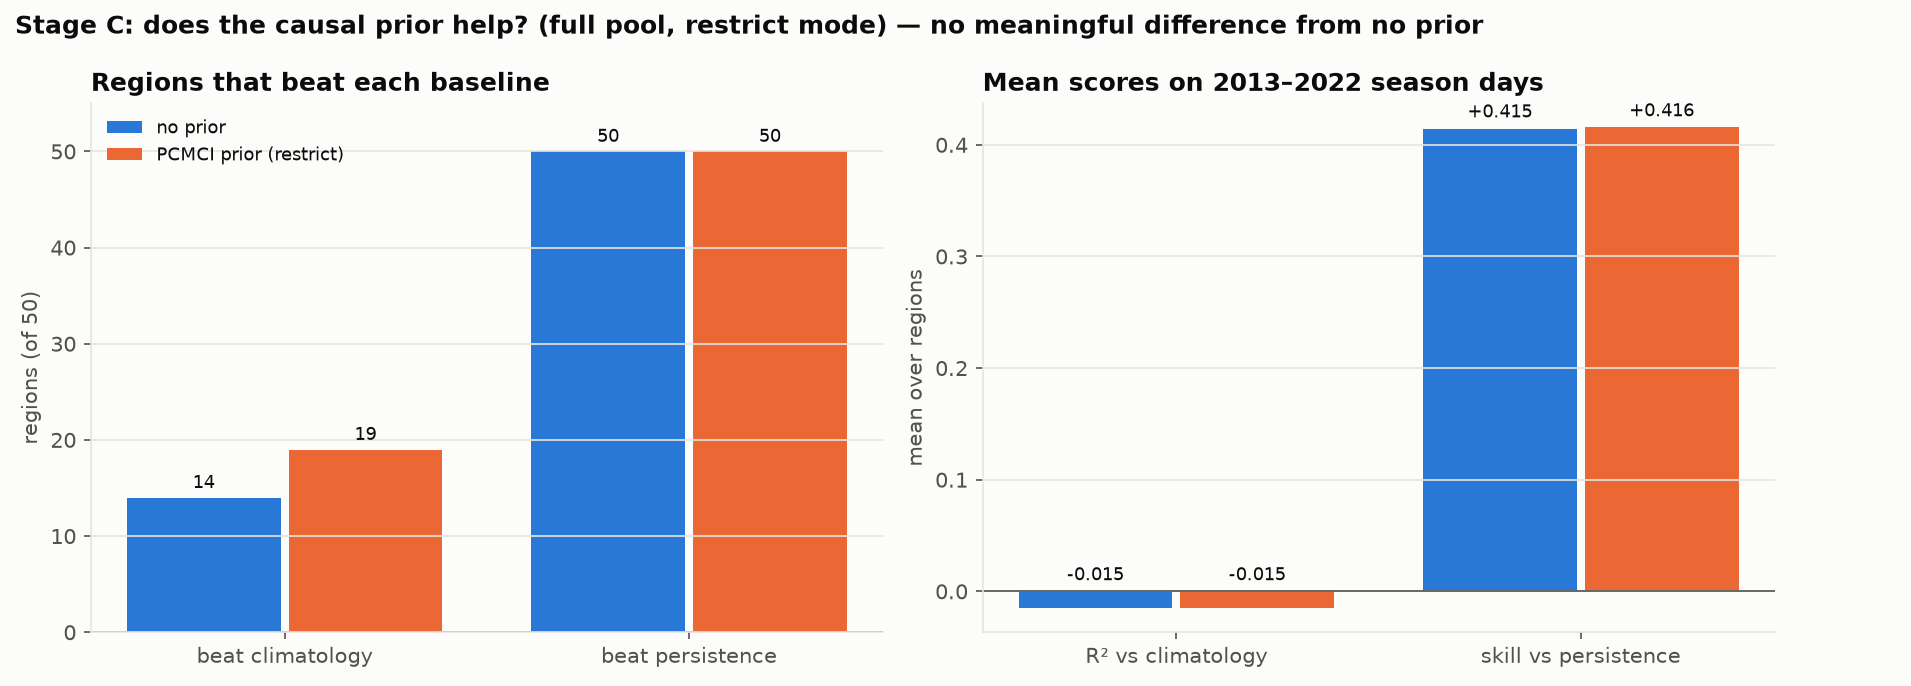
\includegraphics[width=0.92\textwidth]{09_stage_c_pcmci_vs_none.png}
\caption{Seven-day lead, full pool: regions beating each baseline (left) and mean scores (right), with and without the PCMCI restrict prior.}
\label{fig:stagec7}
\end{figure}

\paragraph{Dependence on prior size.} The one-day gain varies with prior size. The two targets with an empty prior, which are restricted to their own region, improve most ($S_{\mathrm{pers}}$ from $-0.86$ to $+0.52$); targets with two or more prior regions improve on average ($-1.53\to-0.91$ for two, $-1.53\to-1.22$ for three or more); and targets with a single prior region worsen ($-1.63\to-2.48$), because the splitter must then choose between the target's own history and its single driver. Comparing with random priors of equal size, the next step of the experimental programme, will separate the contribution of the graph's choice of regions from that of the smaller pool.

\section{Drift Detection (RQ4)}
\label{sec:res-drift}

Table~\ref{tab:drift} reports the four detector settings on an abrupt shift (the 1997--98 El Ni\~{n}o) and a gradual shift (2013--2022) at three regions.

\begin{table}[htbp]
\centering
\caption{Drift detection latency (days from the start of the shift window to the first alarm in it) and false-alarm rate (alarms per year outside all known shift events).}
\label{tab:drift}
\scriptsize
\setlength{\tabcolsep}{3.5pt}
\begin{tabular}{llcccc}
\toprule
\textbf{Region} & \textbf{Shift} & \textbf{Ch.\,1 error} & \textbf{Ch.\,2 structure} & \textbf{Fused OR} & \textbf{Fused AND} \\
\midrule
22 & abrupt 1997--98 & 159 d & \textbf{35 d} & 35 d & missed \\
   & gradual 2013--22 & 966 d & \textbf{181 d} & 181 d & 966 d \\
29 & abrupt 1997--98 & 223 d & \textbf{92 d} & 92 d & 235 d \\
   & gradual 2013--22 & 1{,}158 d & \textbf{117 d} & 117 d & 1{,}195 d \\
12 & abrupt 1997--98 & \textbf{95 d} & 123 d & 95 d & 123 d \\
   & gradual 2013--22 & \textbf{70 d} & 100 d & 70 d & 100 d \\
\midrule
\multicolumn{2}{l}{False alarms per year (22 / 29 / 12)} & 0.17 / 0.34 / 1.04 & 1.62 / 2.25 / 2.19 & 1.78 / 2.59 / 3.23 & 0.17 / 0.34 / 0.94 \\
\bottomrule
\end{tabular}
\end{table}

All shifts are detected by the OR fusion at every region. At regions 22 and 29 the causal-structure channel detects the abrupt El Ni\~{n}o shift 2.4--4.5 times sooner than the error channel, and the gradual shift 5.3--9.9 times sooner, which supports H4: watching the causal structure can reveal a change before it shows in the forecast error. At region 12 the error channel is faster. The structure channel raises more false alarms, so the fusion rule is a genuine trade-off between speed (OR) and caution (AND).

\section{Expert Lifecycle (RQ4)}
\label{sec:res-lifecycle}

Over 1979--2022, the lifecycle handled 49--61 regime changes per region. In \textbf{104 of 171} (61\%) an archived expert matched the new regime and was reactivated instead of a fresh expert being trained (Figure~\ref{fig:timeline}): regimes recur, and the archive reuses what was learned about them, supporting H5.

\begin{figure}[htbp]
\centering
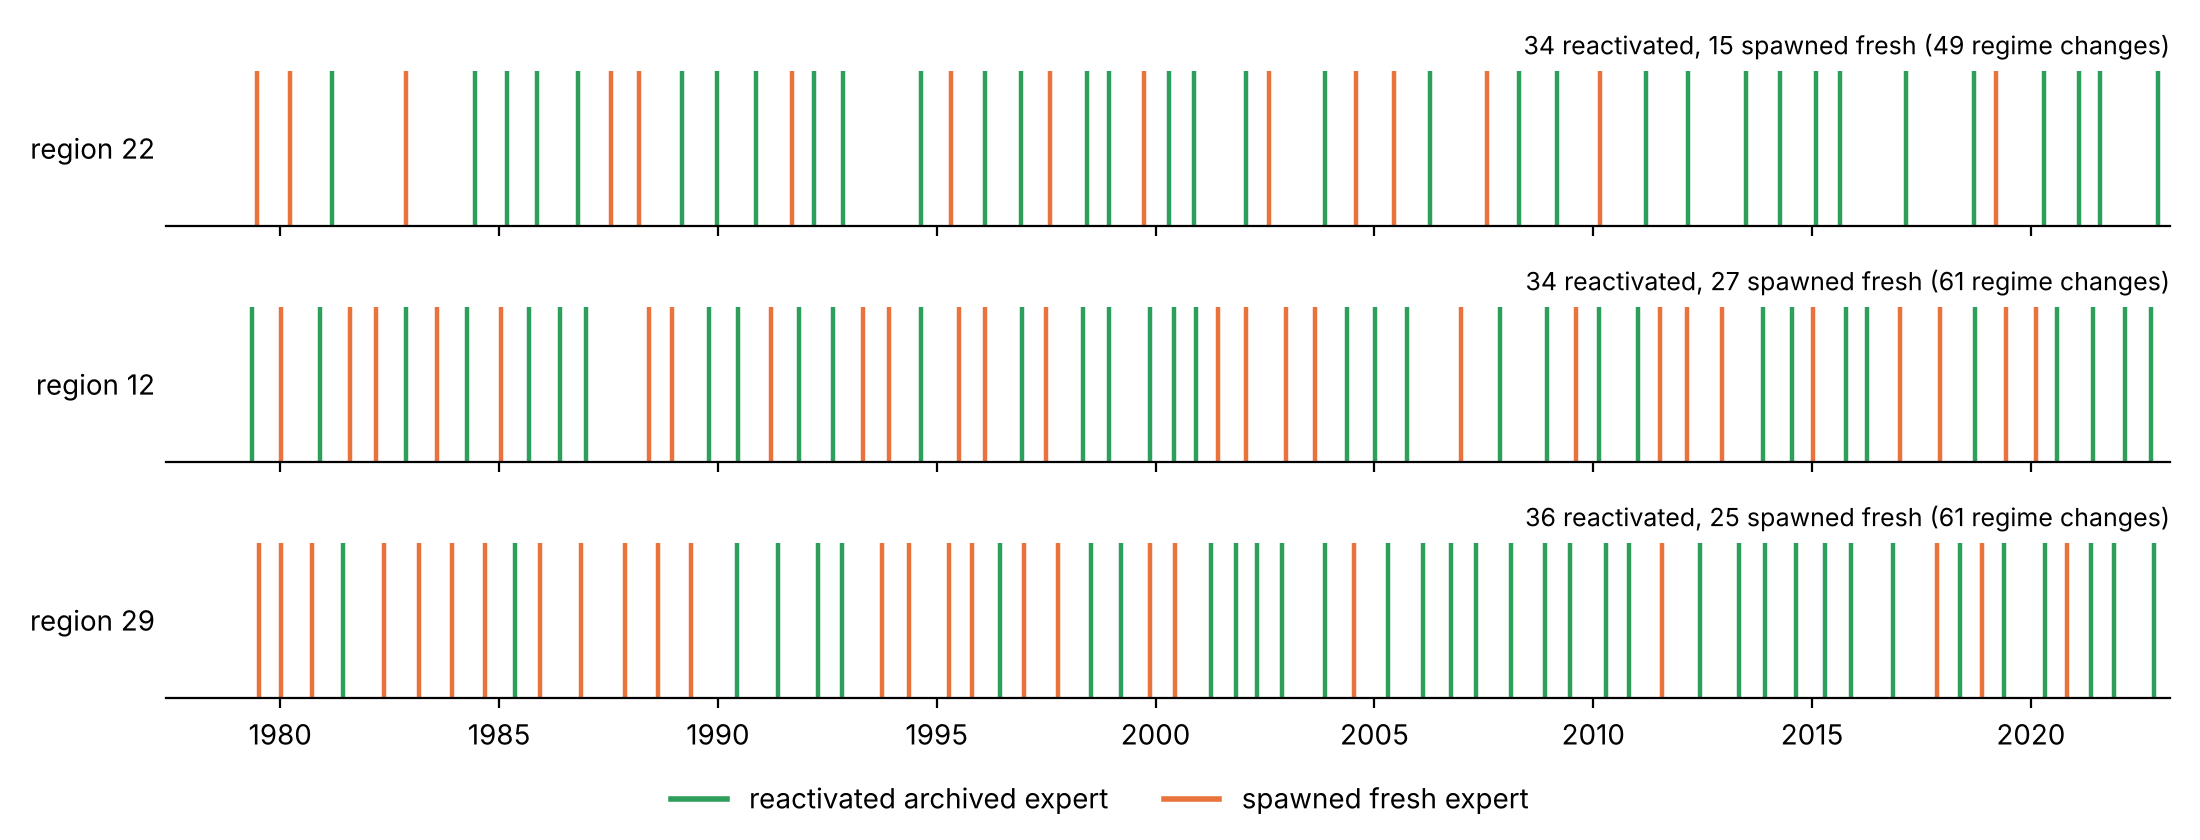
\includegraphics[width=\textwidth]{11_lifecycle_timeline.png}
\caption{Expert lifecycle events, 1979--2022: reactivation of an archived expert (green) or spawning of a fresh expert (orange) at each detected regime change, for regions 22, 12 and 29.}
\label{fig:timeline}
\end{figure}

\begin{table}[htbp]
\centering
\caption{Reactivation strategies: single best-matching archived expert vs a similarity-weighted blend of the top three.}
\label{tab:pool-blend}
\footnotesize
\begin{tabular}{lccc}
\toprule
 & \textbf{Region 22} & \textbf{Region 12} & \textbf{Region 29} \\
\midrule
Blend beats single (events) & 30/49 (61\%) & 42/61 (69\%) & 41/61 (67\%) \\
Mean MSE: single $\to$ blend & 0.368 $\to$ \textbf{0.352} & 0.422 $\to$ \textbf{0.402} & 0.384 $\to$ \textbf{0.376} \\
Forgetting: single $\to$ blend & $-0.010\to\mathbf{-0.013}$ & $0.183\to\mathbf{0.170}$ & $0.092\to\mathbf{0.086}$ \\
\bottomrule
\end{tabular}
\end{table}

Blending the three most similar archived experts beats reactivating the single best match on both forecast error and forgetting at all three regions (Table~\ref{tab:pool-blend}). Whether a reactivated expert should be warm-started from its archived weights or trained fresh depends on the region (Figure~\ref{fig:forget}): warm-starting gives lower forecast error in 28 of 34 events at region 22 and 24 of 36 at region 29, but lower forgetting only at region 29.

\begin{figure}[htbp]
\centering
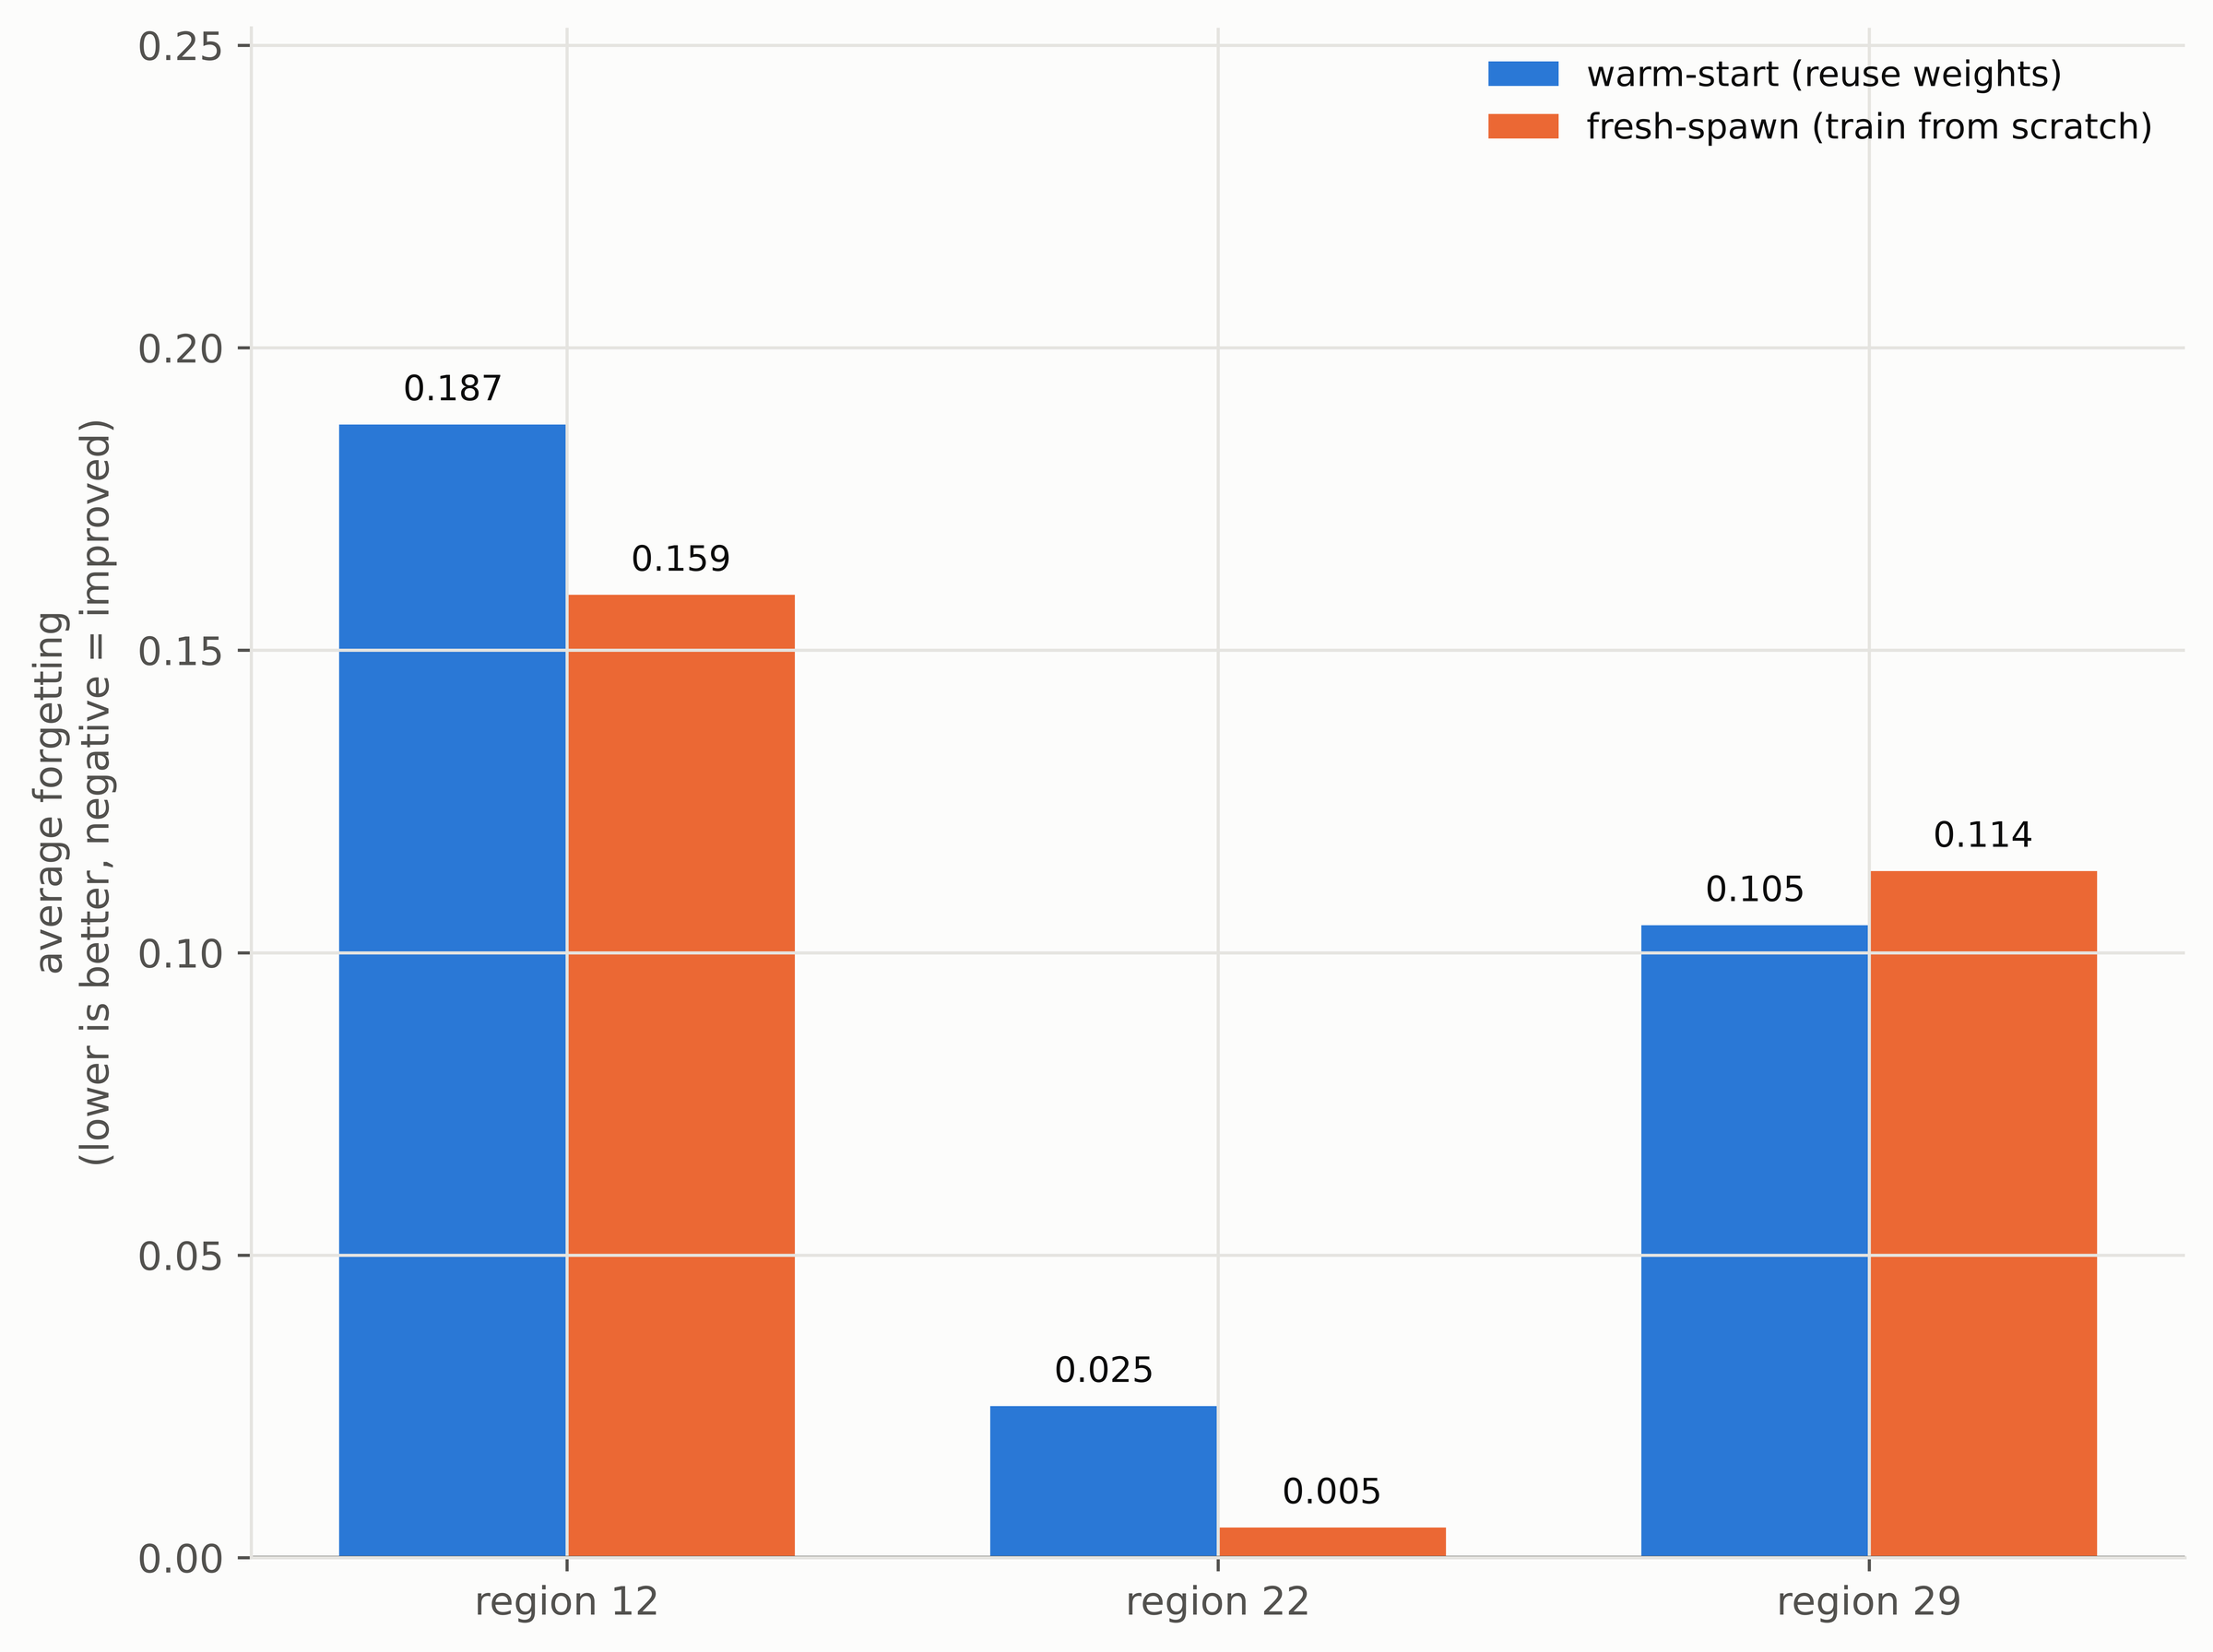
\includegraphics[width=0.62\textwidth]{ppt_forgetting_warm_vs_fresh_3regions_fixed.png}
\caption{Average forgetting (lower is better) when a reactivated expert is warm-started from its archived weights or trained fresh.}
\label{fig:forget}
\end{figure}

\section{Stage D: Structural Drift of the PCMCI Graph}
\label{sec:res-staged}

A Ni\~{n}o-3.4 proxy computed from the project's own SST matches the known ENSO phase in 22 of 24 labelled years. With one-season windows, the parent-set distance is 0.164 when the ENSO phase changes and 0.151 when it does not (Mann--Whitney $p=0.20$); with three-season windows it is 0.200 versus 0.207 ($p=0.76$). Each window has only one or two parents per target, so set membership changes mainly through sampling noise (Figure~\ref{fig:staged}).

\begin{figure}[htbp]
\centering
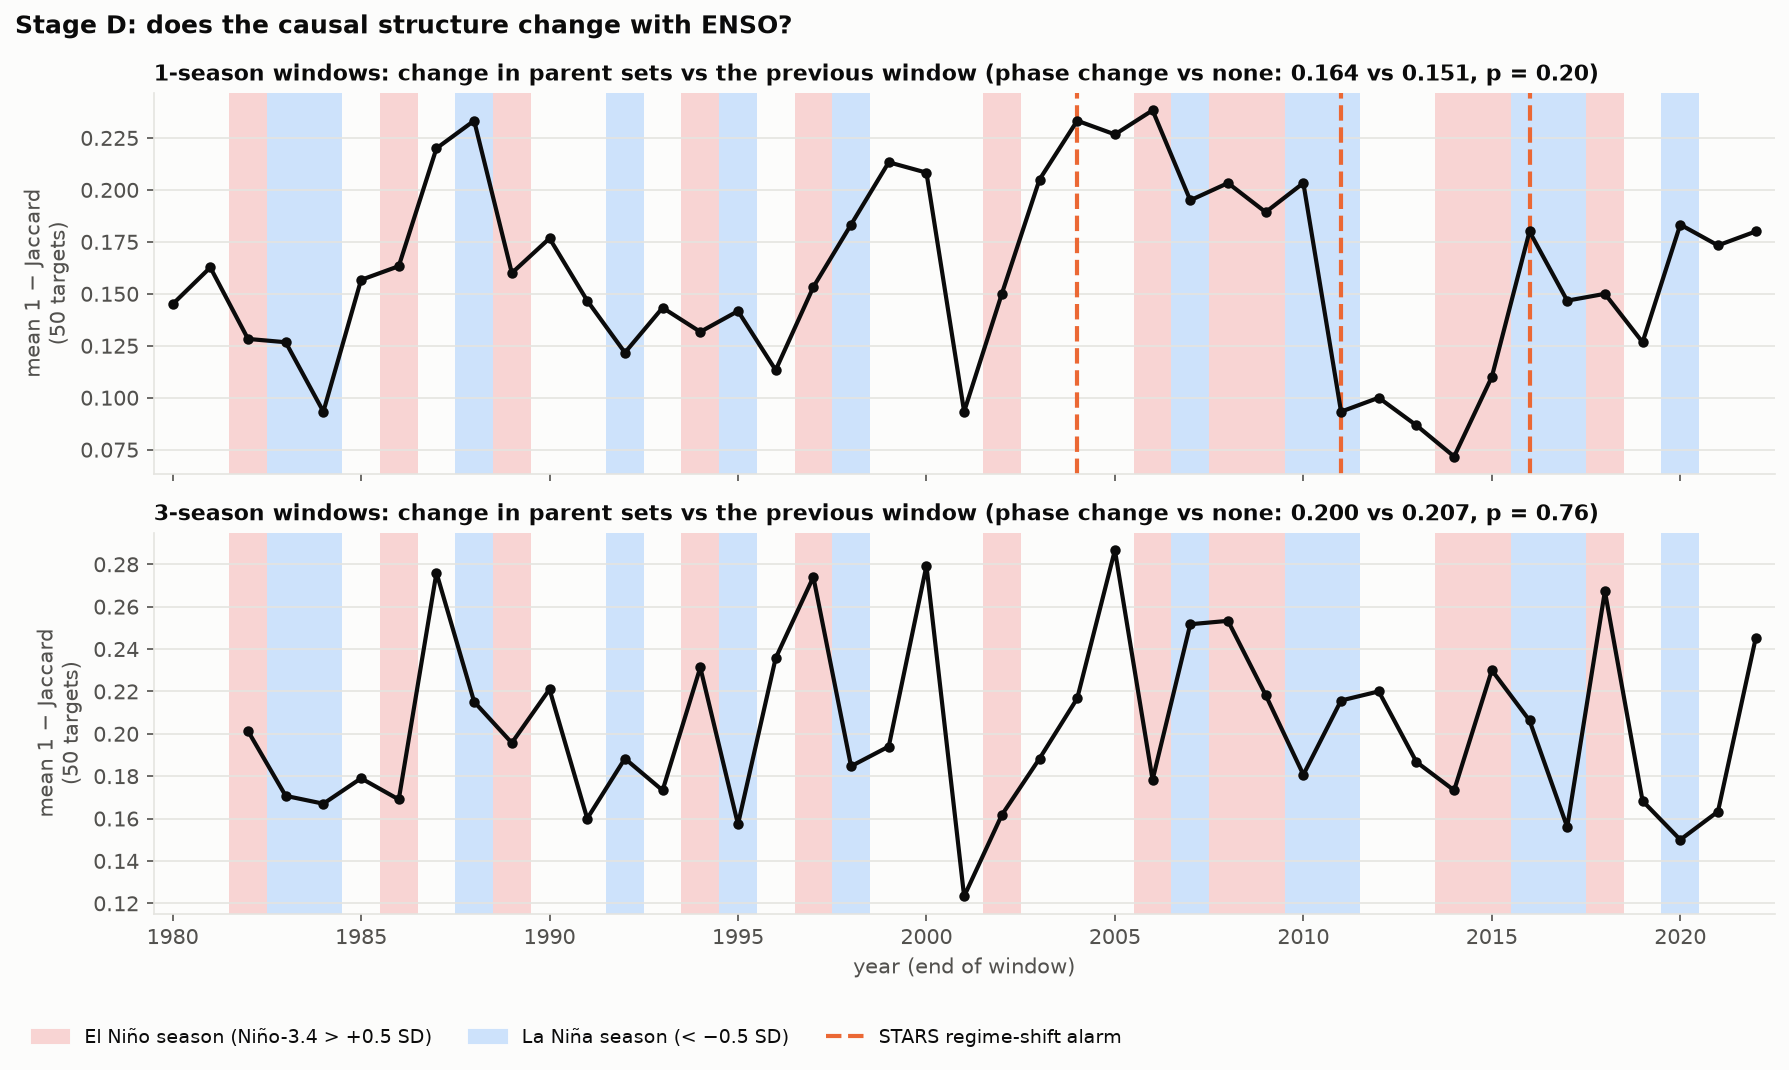
\includegraphics[width=\textwidth]{08_stage_d_drift.png}
\caption{Stage~D: mean parent-set distance between consecutive one-season (top) and three-season (bottom) windows, with El Ni\~{n}o (red) and La Ni\~{n}a (blue) seasons shaded and STARS alarms dashed.}
\label{fig:staged}
\end{figure} Unlike the splitter-score signal of Section~\ref{sec:res-drift}, the discrete PCMCI parent set is therefore not a reliable regime signal at these window lengths; longer windows and strength-based distances are the natural next step.

\section{Summary of Findings}
\label{sec:res-interpret}

\begin{table}[htbp]
\centering
\caption{Outcome of the hypotheses.}
\label{tab:hyp-outcome}
\footnotesize
\renewcommand{\arraystretch}{1.2}
\begin{tabularx}{\textwidth}{>{\raggedright\arraybackslash}p{3.6cm}>{\raggedright\arraybackslash}X>{\raggedright\arraybackslash}p{2.6cm}}
\toprule
\textbf{Hypothesis} & \textbf{Evidence} & \textbf{Outcome} \\
\midrule
H1 Credibility & 0/250 decoys; 3/536 speed violations & Supported \\
H2 Resolution persistence & 33/48 targets $\ge$ 0.5; mean 0.62 & Supported \\
H3 Graph prior helps & Informative splitters 0 $\to$ 24 (7 d) and 0 $\to$ 36 (1 d); 1-day skill better in 32/50 regions; 7-day skill unchanged & Supported at 1 day \\
H4 Earlier detection & Structure channel 2.4--9.9$\times$ faster at regions 22 and 29 & Supported at 2 of 3 regions \\
H5 Regime reuse & 104/171 changes reactivated an archived expert; blend best & Supported \\
\bottomrule
\end{tabularx}
\end{table}

\section{Limitations}
\label{sec:res-validity}

\begin{itemize}
  \item \textbf{No ground truth.} The checks can reject a bad graph but cannot prove a graph correct; every causal claim is a statement of conditional dependence between region means.
  \item \textbf{Hidden drivers and power.} PCMCI assumes all common drivers are observed; BSISO phase, ENSO and moisture are only partly captured. With 18{,}000 candidates per target, some links are missed and some false links remain.
  \item \textbf{Time-scale match.} The validated links act within one or two days, shorter than the 7-day lead; a graph built with lags of at least seven days is needed for week-ahead guidance.
  \item \textbf{Evaluation scope.} The forecasting comparisons use a single training seed and compare against the no-prior model; the drift and lifecycle results cover three regions. The upstream climatology (1979--2014) overlaps the test period by two years.
  \item \textbf{Absolute skill at 7 days.} At seven days the models beat persistence everywhere but not climatology on average ($R^2_{\mathrm{clim}}\approx-0.015$).
\end{itemize}

\section{Implications for Phase 2}
\label{sec:res-implications}

Phase~2 keeps the validation pipeline (decoys, speed mask, persistence), the activity-based season and the region-level prior; builds graphs with lags matched to the forecast lead; uses the dual-channel detector with continuous structure signals; and adopts pooled reactivation of archived experts as the default lifecycle action.

\chapter{Phase 2: India-Focused Forecasting and Adaptive Experts}
\label{chap:phase2}

This chapter describes Phase~2, which carries the Phase~1 lessons into an India-focused regional forecasting system with causal gating and adaptive experts. It combines the regional-forecasting and adaptation components of the research plan into one extension. Section~\ref{sec:p2-status} separates what has been implemented from what is designed and what is future work; unless stated otherwise, the content of this chapter is a design specification.

\section{Motivation: From Regional OLR to Forecasting over India}
\label{sec:p2-motivation}

Phase~1 studied a deliberately simplified problem: a single convective proxy, daily resolution, 50 large regions and a small forecaster. This made it possible to test the causal graph with full control. Its findings, however, matter most if they help a forecast that people use. India is a natural setting for the extension:
\begin{itemize}
  \item The BSISO studied in Phase~1 drives the active and break spells of the Indian summer monsoon~\cite{goswami2001intraseasonal,annamalai2001active}, so the large-scale drivers identified there are physically relevant.
  \item High-resolution regional reanalysis (IMDAA~\cite{rani2021imdaa}) and dense station records~\cite{smith2011integrated} make kilometre-scale, hourly evaluation possible.
  \item Near-surface heat, humidity and wind over India have strong societal impact, and their predictability changes with monsoon regime and ENSO state~\cite{kumar1999weakening}, which makes adaptation to shift a real requirement.
\end{itemize}
The question for Phase~2 is: \emph{can the causal architecture contribute to a competitive hourly forecasting system over India up to 72 hours ahead, and can it adapt when the regional climate relationships change?}

\section{Forecasting Targets, Resolution and Horizon}
\label{sec:p2-targets}

Table~\ref{tab:p2-targets} lists the planned targets. Gridded targets are near-surface fields on a regional grid of about 0.12\dg\ (about 12\,km), matching the IMDAA reanalysis. Point targets are station observations, used to evaluate the gridded forecasts where they matter most and, optionally, as direct forecast targets.

\begin{table}[htbp]
\centering
\caption{Planned Phase~2 forecast targets.}
\label{tab:p2-targets}
\footnotesize
\renewcommand{\arraystretch}{1.2}
\begin{tabularx}{\textwidth}{>{\raggedright\arraybackslash}p{3.5cm}>{\raggedright\arraybackslash}p{2.4cm}>{\raggedright\arraybackslash}X}
\toprule
\textbf{Target} & \textbf{Type} & \textbf{Notes} \\
\midrule
2\,m temperature & Gridded, station & Diurnal cycle and heat-wave relevance \\
2\,m relative humidity & Gridded & Heat stress; monsoon moisture \\
10\,m zonal and meridional wind & Gridded & Monsoon flow; wind energy \\
Mean sea-level pressure & Gridded & Synoptic systems, monsoon trough and depressions \\
2\,m dewpoint & Station & Moisture at observation sites \\
\midrule
\multicolumn{3}{l}{Temporal resolution: hourly. Horizon: 1--72 hours. Domain: Indian region at about 0.12\dg\ ($\approx$12\,km).}\\
\bottomrule
\end{tabularx}
\end{table}

Two features distinguish this task from Phase~1. The horizon is short (up to three days), so the short-lag dependencies that Phase~1 found are exactly the ones that matter. And the targets are dominated by the diurnal cycle and by local surface conditions, so a strong shared model of local dynamics is required before any remote driver can add value.

\section{Proposed Datasets and Their Roles}
\label{sec:p2-data}

Table~\ref{tab:p2-data} lists the candidate datasets. Their versions, periods, licences and acquisition status must be confirmed before they are treated as final choices; the decision log (Appendix~\ref{app:decisions}) records them as open.

\begin{table}[htbp]
\centering
\caption{Candidate Phase~2 datasets. All entries are planned; versions, periods and licences are to be confirmed.}
\label{tab:p2-data}
\footnotesize
\renewcommand{\arraystretch}{1.2}
\begin{tabularx}{\textwidth}{>{\raggedright\arraybackslash}p{2.3cm}>{\raggedright\arraybackslash}p{3.3cm}>{\raggedright\arraybackslash}X}
\toprule
\textbf{Dataset} & \textbf{Characteristics} & \textbf{Role} \\
\midrule
IMDAA~\cite{rani2021imdaa} & Regional reanalysis for the Indian monsoon region; about 12\,km; hourly; satellite era & Primary gridded inputs and targets over India \\
ERA5~\cite{hersbach2020era5} & Global reanalysis; about 31\,km (0.25\dg); hourly; 1940 onward & Boundary context outside the regional domain; source of candidate large-scale drivers (for example BSISO, ENSO and Indian Ocean indices, remote circulation) \\
NOAA ISD~\cite{smith2011integrated} & Hourly and synoptic station observations worldwide & Independent point verification; station targets (2\,m temperature, dewpoint) \\
\bottomrule
\end{tabularx}
\end{table}

Station data require explicit quality control (duplicate removal, outlier and gap handling, station relocation checks) and a policy for matching stations to grid cells. Reanalysis data require consistent regridding, unit harmonisation and alignment of hourly time stamps. As in Phase~1, all statistics used to normalise the data must be estimated on training years only.

\section{Shared Forecasting Backbone}
\label{sec:p2-backbone}

Phase~1 used one small expert per region and no shared model. At kilometre scale and hourly resolution this would discard the common physics shared by all locations. Phase~2 therefore introduces a shared backbone $B_\phi$ that maps the recent regional state to a latent representation for each grid node,
\begin{equation}
  \mathbf{z}_{n,t} = B_\phi\big(\mathbf{x}_{\mathcal{N}(n),\,t-H:t}\big),
\end{equation}
where $\mathcal{N}(n)$ is a local neighbourhood of node $n$ on the regional mesh and $H$ the input history. A graph-based limited-area model~\cite{oskarsson2023graph} or a regional adaptation of a message-passing global model~\cite{keisler2022forecasting,lam2023learning} is a natural choice. The backbone carries the bulk of forecasting skill; the experts and the causal gate add regime-specific and driver-specific corrections.

\section{Candidate Climate Drivers and Lagged Causal Discovery}
\label{sec:p2-drivers}

A \emph{causal detector} identifies which large-scale drivers, and at what lags, carry information about each regional target after conditioning on local history. The candidate drivers come from ERA5 and Phase~1-style regional means: intraseasonal indices (BSISO1/2 amplitude and phase), ENSO and Indian Ocean SST indices, upstream moisture transport, and the state of the large-scale regions identified as drivers in Phase~1. The detector applies the Phase~1 pipeline with three changes motivated by the Phase~1 results:
\begin{enumerate}
  \item \textbf{Lead-matched lags.} For a forecast at lead $L$, drivers are tested only at lags $\tau\ge L$, so that every retained link is usable at the issue time (Eq.~\eqref{eq:availability}).
  \item \textbf{Driver-level priors.} Claims are made at the level of drivers and source regions rather than individual fields, as in the region-level prior of Phase~1.
  \item \textbf{Validation retained.} Decoys, the physical speed mask and resolution persistence are applied as in Phase~1; persistence is tested between the regional grid and a coarser aggregation.
\end{enumerate}
Because hourly data are much more strongly autocorrelated than daily data, the effective sample size per hour of data is low. Discovery can be carried out on daily or six-hourly aggregates of the drivers, with the target aggregated to the same resolution, and the resulting graph applied to the hourly model.

\section{Graph-Guided Gating and Expert Architecture}
\label{sec:p2-gating}

Figure~\ref{fig:p2-arch} shows the planned architecture. Experts $\{E_k\}_{k=1}^{K}$ are small networks that refine the backbone's representation for particular regimes or sub-regions. A gate $g$ assigns weights to the experts for each node and time,
\begin{equation}
  \hat{\mathbf{y}}_{n,t+L} = D_\omega(\mathbf{z}_{n,t}) + \sum_{k=1}^{K} g_k(\mathbf{z}_{n,t},\mathbf{c}_{n,t})\,E_k(\mathbf{z}_{n,t},\mathbf{c}_{n,t}),\qquad \sum_k g_k=1,
  \label{eq:p2moe}
\end{equation}
where $D_\omega$ is the backbone's decoder and $\mathbf{c}_{n,t}$ is a \emph{causal context} vector: the values, at the issue time, of the drivers that the causal detector retained for node $n$, weighted by their link strengths. The gate is sparse (top-1 or top-2 routing~\cite{shazeer2017outrageously,fedus2022switch}) with a load-balancing penalty.

This differs from the Phase~1 use of the graph in an important way. In Phase~1 the graph selected \emph{predictors}: it decided which source regions entered the forecast. In Phase~2 the graph conditions the \emph{gate}: it decides which expert's correction to apply, given the state of the drivers. A driver that is too slow or too remote to add predictive information directly can still be useful for identifying the regime, for example whether the BSISO is in an active phase over India, in which a particular expert is reliable.

\begin{figure}[htbp]
\centering
\resizebox{\textwidth}{!}{%
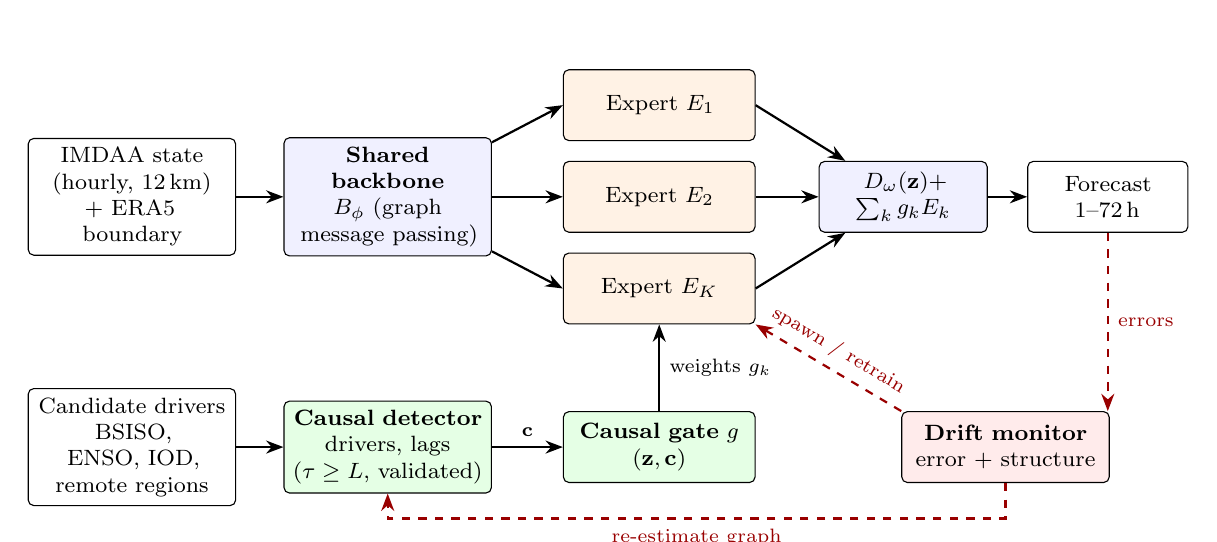
\begin{tikzpicture}[node distance=0.4cm and 0.5cm]
\node[box, text width=2.4cm] (in) {IMDAA state\\(hourly, 12\,km)\\+ ERA5 boundary};
\node[box, fill=blue!6, right=0.6cm of in, text width=2.4cm] (bb) {\textbf{Shared backbone}\\$B_\phi$ (graph\\message passing)};
\node[box, fill=orange!10, right=0.9cm of bb, text width=2.2cm] (e2) {Expert $E_2$};
\node[box, fill=orange!10, above=0.25cm of e2, text width=2.2cm] (e1) {Expert $E_1$};
\node[box, fill=orange!10, below=0.25cm of e2, text width=2.2cm] (e3) {Expert $E_K$};
\node[box, fill=blue!6, right=0.8cm of e2, text width=1.9cm] (sum) {$D_\omega(\mathbf z)+$\\$\sum_k g_k E_k$};
\node[box, right=0.5cm of sum, text width=1.8cm] (out) {Forecast\\1--72\,h};
\node[box, fill=green!10, below=1.1cm of e3, text width=2.2cm] (gate) {\textbf{Causal gate} $g$\\$(\mathbf z,\mathbf c)$};
\node[box, fill=green!10, text width=2.4cm] (cd) at (bb |- gate) {\textbf{Causal detector}\\drivers, lags\\($\tau\ge L$, validated)};
\node[box, text width=2.4cm] (drv) at (in |- gate) {Candidate drivers\\BSISO, ENSO, IOD,\\remote regions};
\coordinate (mid) at ($(sum.south)!0.5!(out.south)$);
\node[box, fill=red!8, text width=2.4cm] (drift) at (mid |- gate) {\textbf{Drift monitor}\\error + structure};
\draw[arr] (in) -- (bb); \draw[arr] (bb) -- (e1.west); \draw[arr] (bb) -- (e2); \draw[arr] (bb) -- (e3.west);
\draw[arr] (e1.east) -- (sum); \draw[arr] (e2) -- (sum); \draw[arr] (e3.east) -- (sum); \draw[arr] (sum) -- (out);
\draw[arr] (drv) -- (cd); \draw[arr] (cd) -- node[lbl,above]{$\mathbf c$} (gate);
\draw[arr] (gate) -- node[lbl,right]{weights $g_k$} (e3);
\draw[darr, red!60!black] (out.south) -- node[lbl,right]{errors} (out.south |- drift.north);
\draw[darr, red!60!black] (drift.north west) -- node[lbl, sloped, above]{spawn / retrain} (e3.south east);
\draw[darr, red!60!black] (drift.south) -- ++(0,-0.45) -| node[lbl, pos=0.25, below]{re-estimate graph} (cd.south);
\end{tikzpicture}%
}
\caption{Planned Phase~2 architecture (schematic). A shared backbone encodes the regional state; a causal detector provides validated, lead-matched drivers that condition a sparse gate over experts; a drift monitor watches forecast errors and causal structure, and triggers re-estimation of the graph and the creation, retraining or reactivation of experts.}
\label{fig:p2-arch}
\end{figure}

\paragraph{Open design choices.} The design documents admit several expert structures, and none has been finalised: (i) \emph{regional experts}, one per sub-region of India (for example by homogeneous rainfall zones); (ii) \emph{per-node experts} with shared parameters and node embeddings; (iii) \emph{regime experts} shared across space and selected by the causal context; or (iv) a hybrid of a shared expert and regime experts. Option (iii) uses the causal context most directly; option (i) is closest to Phase~1. The choice will be made on validation data, and the alternatives are recorded in the decision log.

\section{Drift Monitoring and Causal-Signature Changes}
\label{sec:p2-drift}

A deployed regional model faces three kinds of change: \emph{seasonal} changes that recur every year, \emph{interannual regime} changes such as ENSO phases, and \emph{long-term} changes due to climate trends or changes in the observing system. The model should not react to the first (it can be learned), should adapt to the second, and should be retrained for the third.

Two monitoring channels are planned:
\begin{enumerate}
  \item \textbf{Error channel.} The rolling forecast error of each expert is monitored with ADWIN~\cite{bifet2007learning}, which keeps a variable-length window and signals a change when two sub-windows have significantly different means, or with CUSUM~\cite{page1954continuous}:
  \begin{equation}
    C_t = \max\big(0,\;C_{t-1}+(e_t-\mu_0-\kappa)\big),\qquad \text{alarm if } C_t>h,
  \end{equation}
  where $e_t$ is the error, $\mu_0$ its reference mean, $\kappa$ a slack and $h$ a threshold.
  \item \textbf{Structure channel.} The causal detector is rerun on rolling windows and the change in the driver set or driver strengths is monitored with STARS~\cite{rodionov2004sequential}. Phase~1 showed that a set-based Jaccard distance on short windows is dominated by sampling noise, so Phase~2 uses a strength-based distance over longer windows against a fixed reference,
  \begin{equation}
    \Delta^{\mathrm{str}}_{w} = \frac{\lVert \mathbf{m}_w-\mathbf{m}_{\mathrm{ref}}\rVert_1}{\lVert\mathbf{m}_{\mathrm{ref}}\rVert_1},
  \end{equation}
  where $\mathbf{m}_w$ is the vector of MCI strengths of the candidate links in window $w$.
\end{enumerate}
STARS computes, for each new observation, a regime-shift index
\begin{equation}
  \mathrm{RSI}_{t} = \sum_{s=t}^{t+m}\frac{x_s-\bar{x}_{\mathrm{new}}}{\ell\,\hat\sigma_{\ell}},
\end{equation}
where $\bar{x}_{\mathrm{new}}$ is the critical level that a new regime's mean must exceed (set from a $t$-test at a chosen significance level), $\ell$ is the cut-off length and $\hat\sigma_\ell$ the average standard deviation of $\ell$-length intervals; a shift is accepted if the index keeps its sign over the cut-off length~\cite{rodionov2004sequential}. The two channels can be combined with OR, which reacts quickly at the cost of more false alarms, or with AND, which is more conservative.

\section{Regime-Shift Detection and Selective Expert Adaptation}
\label{sec:p2-adapt}

When a drift alarm is raised for a region or regime, the lifecycle of the affected expert is decided in tiers:
\begin{itemize}
  \item \textbf{Tier 0, no action:} the alarm is not confirmed by the second channel, or the error is within its normal range.
  \item \textbf{Tier 1, retrain:} the expert is fine-tuned on recent data, with an elastic-weight-consolidation penalty~\cite{kirkpatrick2017overcoming} to limit forgetting of earlier regimes.
  \item \textbf{Tier 2, spawn or reactivate:} the current expert is archived together with its causal signature, and either a new expert is spawned or an archived expert is reactivated.
\end{itemize}
Archived experts are retrieved by the similarity of their causal signature to the current one. Two retrieval rules are compared: \emph{single best match}, which reactivates the most similar archived expert, and \emph{pool blend}, which blends the $k$ most similar experts with weights proportional to their similarity. Because climate regimes such as El Ni\~{n}o recur, reactivation reuses knowledge rather than relearning it, and adding experts instead of overwriting them avoids catastrophic forgetting~\cite{rusu2016progressive,aljundi2017expert}.

\section{Groundwork Implemented on the Phase 1 Dataset}
\label{sec:p2-groundwork}

The drift-monitoring and expert-lifecycle machinery has been implemented and tested on the Phase~1 daily OLR data, using the splitter's edge-score pattern as the structural signal (rather than the PCMCI parent sets of Stage~D), at three regions chosen to span low, medium and high splitter discrimination (regions 22, 12 and 29). These experiments are the groundwork for the Phase~2 lifecycle.

\paragraph{Drift detection.} Two test shifts were used: the abrupt 1997--98 El Ni\~{n}o and a gradual multi-year shift. Table~\ref{tab:p2-drift} shows the results for region 22. The error channel alone missed the abrupt shift and detected the gradual one slowly; the structure channel detected both quickly; their OR combination detected both quickly; their AND combination missed the abrupt shift. At regions 12 and 29, both shifts were detected under all signal and combination settings, with region-specific delays; at region 29 the structure channel detected the gradual shift after 117 days, compared with 1{,}158 days for the error channel.

\begin{table}[htbp]
\centering
\caption{Drift detection on two test shifts, region 22 (Phase~1 data, splitter-score structure signal).}
\label{tab:p2-drift}
\small
\renewcommand{\arraystretch}{1.15}
\begin{tabular}{lcc}
\toprule
\textbf{Detector} & \textbf{Abrupt shift (1997--98)} & \textbf{Gradual shift} \\
\midrule
Error channel only & missed & detected, slowly \\
Structure channel only & detected, quickly & detected \\
OR combination & detected, quickly & detected \\
AND combination & missed & detected, slowly \\
\bottomrule
\end{tabular}
\end{table}

\paragraph{Expert retrieval.} Table~\ref{tab:p2-lifecycle} compares the two retrieval rules and the choice between warm-starting a reactivated expert and spawning a fresh one. Blending the three most similar archived experts beat reactivating the single best match on forecast error in 61--69\% of drift events and on forgetting at all three regions, which is the most consistently repeated finding of these experiments. Whether warm-starting helps is region-dependent.

\begin{table}[htbp]
\centering
\caption{Expert lifecycle comparisons on Phase~1 data at three regions. Fractions are drift events in which the first option has lower forecast error.}
\label{tab:p2-lifecycle}
\footnotesize
\renewcommand{\arraystretch}{1.2}
\begin{tabular}{p{6.6cm}ccc}
\toprule
\textbf{Comparison} & \textbf{Region 22} & \textbf{Region 12} & \textbf{Region 29} \\
\midrule
Pool blend beats single best (forecast error) & 30/49 (61\%) & 42/61 (69\%) & 41/61 (67\%) \\
Pool blend better on forgetting & yes & yes & yes \\
Warm start beats fresh spawn (forecast error) & 28/34 (82\%) & mixed & 24/36 (67\%) \\
Warm start better on forgetting & no & no & yes \\
\bottomrule
\end{tabular}
\end{table}

\paragraph{Reconciling the two structural signals.} The splitter-score signal detected the two test shifts, whereas the PCMCI parent-set distance of Stage~D did not track ENSO across all years. The two results are not contradictory: they use different signals (continuous splitter scores versus discrete parent sets), different tests (two named events at three regions versus all phase changes at fifty regions) and different window lengths. Together they suggest that continuous, strength-based structural signals are more promising than set-based ones, which is the choice made for Phase~2 (Section~\ref{sec:p2-drift}).

\section{Evaluation under Distribution Shift}
\label{sec:p2-eval}

The Phase~2 evaluation protocol follows the Phase~1 discipline of chronological splits, frozen choices and paired comparisons, and adds evaluation that is specific to shift:
\begin{itemize}
  \item \textbf{Temporal holdout:} the most recent years are held out entirely; normalisation, graph discovery and model selection use training years only.
  \item \textbf{Regime-stratified scores:} errors reported separately for El Ni\~{n}o, La Ni\~{n}a and neutral seasons, active and break monsoon phases, monsoon onset and withdrawal, and pre-monsoon heat.
  \item \textbf{Leave-regime-out tests:} training without one regime type and testing on it, to measure generalisation to an unseen regime.
  \item \textbf{Detector metrics:} detection delay after a known shift, false-alarm rate in periods without a shift (with known recurring events counted as true shifts, not false alarms), and the number of lifecycle actions.
  \item \textbf{Adaptation metrics:} error after adaptation, forgetting (the increase of error on earlier regimes after adaptation), and compute cost of retraining.
  \item \textbf{Accuracy metrics:} RMSE, MAE and bias per variable, lead and region; station-based verification against ISD; anomaly correlation for the diurnal-cycle-removed signal.
\end{itemize}

\section{Planned Baselines and Benchmarks}
\label{sec:p2-baselines}

Table~\ref{tab:p2-baselines} lists the planned baselines. The ablations isolate each component: the backbone alone, the backbone with experts but an uninformed gate, the gate with a random or correlation context in place of the causal context, and the full system with and without adaptation.

\begin{table}[htbp]
\centering
\caption{Planned Phase~2 baselines and ablations.}
\label{tab:p2-baselines}
\footnotesize
\renewcommand{\arraystretch}{1.2}
\begin{tabularx}{\textwidth}{>{\raggedright\arraybackslash}p{4.4cm}>{\raggedright\arraybackslash}X}
\toprule
\textbf{Baseline / ablation} & \textbf{Purpose} \\
\midrule
Persistence; diurnal persistence (same hour yesterday) & Lower bounds for hourly forecasts \\
Hourly climatology by day of year & Reference for skill scores \\
Backbone only & Value of experts and gate \\
Backbone + experts, learned gate without causal context & Value of the causal context \\
Gate with random / correlation context of equal size & Specificity of causal information (as in Phase~1) \\
Full system without adaptation & Value of drift-triggered adaptation \\
Periodic retraining on a fixed schedule & Adaptation without drift detection \\
Published global ML forecasts, e.g.\ GraphCast~\cite{lam2023learning}, GenCast~\cite{price2025probabilistic}, interpolated to the regional grid & External benchmark, where forecasts are available for the test period \\
\bottomrule
\end{tabularx}
\end{table}

\section{Implementation Status and Unresolved Design Choices}
\label{sec:p2-status}

Table~\ref{tab:p2-status} records the status of each component.

\begin{table}[htbp]
\centering
\caption{Phase~2 component status.}
\label{tab:p2-status}
\footnotesize
\renewcommand{\arraystretch}{1.2}
\begin{tabularx}{\textwidth}{>{\raggedright\arraybackslash}p{4.3cm}>{\raggedright\arraybackslash}p{3.1cm}>{\raggedright\arraybackslash}X}
\toprule
\textbf{Component} & \textbf{Status} & \textbf{Notes} \\
\midrule
Causal discovery and validation pipeline & Implemented (Phase~1) & To be extended with lead-matched lags and driver indices \\
Error and structure drift channels; STARS; ADWIN & Implemented (Phase~1 data) & Strength-based structure distance to be added \\
Expert archive, reactivation, pool blending & Implemented (Phase~1 data) & Tested at three regions \\
India datasets (IMDAA, ERA5, ISD) & Planned & Versions, periods and licences to be confirmed \\
Shared backbone & Designed & Architecture choice open \\
Causal gate and expert structure & Designed & Regional, per-node, regime or hybrid experts: open \\
Shift-aware evaluation & Designed & Protocol in Section~\ref{sec:p2-eval} \\
External benchmarks & Planned & Depends on forecast availability for the test period \\
\bottomrule
\end{tabularx}
\end{table}

\section{Relationship to the Phase 1 Contribution}
\label{sec:p2-relation}

Phase~2 depends on Phase~1 in three ways. First, it inherits the validated components: the decoy test, the physical speed mask and the persistence test give a way to trust a driver set before using it, and they scale to large candidate pools. Second, it inherits two design corrections: lags must match the forecast lead, and set-based structural signals from short windows are too noisy to drive adaptation. Third, it inherits the evaluation discipline: graphs frozen before testing, matched random and correlation controls, and reporting of neutral and negative results. The question left open by Phase~1, whether the causal content of a graph improves on a random graph of the same size, is equally central to Phase~2, where it becomes the comparison between a causal and a random gate context.

\section{Future Scale-Up Considerations}
\label{sec:p2-scale}

If Phase~2 shows regional value, the approach could be extended to larger domains and eventually to a global mesh. Three issues would then dominate: the cost of causal discovery, which grows with the number of targets times the number of candidates and would require hierarchical or dimension-reduced candidate sets; the number of experts, which must stay bounded through archiving and merging; and evaluation against global data-driven systems on standard benchmarks such as WeatherBench~2~\cite{rasp2024weatherbench2}. Global forecasting is not part of this thesis and is discussed only as a long-term direction (Section~\ref{sec:conc-future}).

\section{Chapter Summary}
\label{sec:p2-summary}

Phase~2 extends the causal-graph approach to hourly, kilometre-scale forecasting of near-surface variables over India up to 72 hours ahead. It combines a shared backbone, a causal detector with lead-matched and validated drivers, a gate conditioned on causal context, and drift-triggered expert adaptation with archiving and reactivation. The drift and lifecycle machinery has been implemented and tested on Phase~1 data, where blending archived experts outperformed single-expert reactivation in a majority of drift events and on forgetting at all three regions tested; the remaining components are designed, with their open choices and evaluation protocol recorded.

\chapter{Conclusion and Scope for Further Research}
\label{chap:conclusion}

\section{Summary of the Scientific Problem}
\label{sec:conc-problem}

Forecasting models choose their predictors by association, and in the tropical atmosphere association is inflated by autocorrelation, shared seasonal cycles and common drivers. This thesis asked whether a graph of lagged dependencies, found by causal discovery, validated by independent checks and frozen before the test years, can tell a forecasting model which source regions to use. The setting was daily OLR, a proxy for deep convection, forecast for 50 tropical regions during the BSISO season, with 1979--2012 for development and 2013--2022 held out.

\section{Summary of the Methods}
\label{sec:conc-methods}

The work built a 300-node representation of six variables over 50 OLR-coherent regions and an activity-based BSISO season from a reproduced BSISO index. It applied PCMCI with partial-correlation tests and Benjamini--Hochberg FDR control to 18{,}000 lagged candidates per target, using a vectorised implementation verified against Tigramite. It validated the graph with four checks: phase-randomised decoys in a separate pass, a physical propagation-speed mask, data-driven top-$k$ selection, and persistence at doubled spatial resolution. It merged the validated links into a region-level prior for an invariance-trained splitter and per-region experts, defined three modes of use and three matched control priors, evaluated the prior on held-out years at 7-day and 1-day leads, and measured the temporal stability of the causal structure against ENSO. Finally, it designed an India-focused hourly extension with causal gating and drift-triggered expert adaptation.

\section{Objective-by-Objective Assessment}
\label{sec:conc-objectives}

\begin{table}[htbp]
\centering
\caption{Assessment of the research objectives.}
\label{tab:objectives}
\footnotesize
\renewcommand{\arraystretch}{1.25}
\begin{tabularx}{\textwidth}{>{\raggedright\arraybackslash}p{2.9cm}>{\raggedright\arraybackslash}X>{\raggedright\arraybackslash}p{2.2cm}}
\toprule
\textbf{Objective} & \textbf{Outcome} & \textbf{Status} \\
\midrule
O1 Data representation & 300 nodes, 1979--2022, development/test split; BSISO index with 11.2\%/7.7\% leading variances; season of 208 days per year on average & Achieved \\
O2 Graph discovery & 536 links over 900{,}000 candidates at FDR 0.05; vectorised PCMCI verified against Tigramite; 23 minutes for 50 targets & Achieved \\
O3 Graph validation & 0/250 decoys; 3/536 speed violations; $k^\ast=10$; mean persistence 0.62 (33/48 targets $\ge$ 0.5) & Achieved \\
O4 Graph use & Region-level prior (2.06 regions per target); restrict, initialise and regularise modes and random and correlation controls implemented and unit-tested & Achieved \\
O5 Forecast evaluation & Restrict prior vs no prior in the full pool at 7 and 1 days reported; remaining cells of the 27-configuration grid to follow & Partly achieved \\
O6 Temporal stability & Causal-signature distance computed; no alignment with ENSO & Achieved (negative result) \\
O7 Extension design & Phase~2 architecture, data, baselines and shift-aware evaluation specified; lifecycle groundwork tested & Achieved (design) \\
\bottomrule
\end{tabularx}
\end{table}

Table~\ref{tab:objectives} summarises the outcome of each objective. Six of the seven objectives are achieved. Objective~O5 is partly achieved: the most informative first comparison has been made, and the remaining comparisons use the same, already tested infrastructure.

\section{Contributions and Evidence}
\label{sec:conc-contrib}

\begin{enumerate}
  \item \textbf{A trustworthy graph.} The Phase~1 graph passes every validation check that binds: no decoy selected among 250, 3 of 536 links physically impossible, 62\% mean persistence at doubled resolution, and independent agreement with the splitter for region 22.
  \item \textbf{A reproduced BSISO index and season} from the project's own data that matches the published variance split.
  \item \textbf{A verified, fast PCMCI implementation} that matches Tigramite and makes an 18{,}000-candidate-per-target analysis take 23 minutes.
  \item \textbf{The graph makes source selection discriminative.} With the restrict prior, the number of informative full-pool splitters rises from 0 to 24 of 50 at 7 days and from 0 to 36 at 1 day.
  \item \textbf{A short-lead forecast improvement over the no-prior model.} At 1 day, the restrict prior improves skill in 32 of 50 regions (mean skill relative to persistence $-1.53\to-1.33$; mean $R^2$ relative to climatology $0.720\to0.745$).
  \item \textbf{A characterisation of the graph's time scale.} Outside links act at one or two days, which explains why the graph helps at 1 day and not at 7.
  \item \textbf{A negative result on structural drift.} Set-based causal signatures from one- and three-season windows do not track ENSO.
  \item \textbf{A Phase~2 design} that transfers the validated components and the lessons on lags and drift signals.
\end{enumerate}

\section{What the Experiments Do and Do Not Establish}
\label{sec:conc-establish}

The experiments establish that PCMCI at full scale produces a sparse, interpretable and robust graph for BSISO-season OLR; that using this graph as a restrict prior makes the splitter's choices discriminative; that at the 7-day lead the prior does not change forecast skill; and that at the 1-day lead it improves skill relative to the no-prior model in most regions.

They do not establish that the graph's links are causal in a mechanistic sense, which no observational check can do. They do not yet establish that the one-day gain comes from the graph's choice of regions rather than from the reduced size of the candidate pool; this is the question answered by the random-prior control. And they do not establish that the causal structure changes with climate regimes in a detectable way. The central Phase~1 hypothesis, that a validated causal graph improves both source selection and forecast skill on unseen years, is therefore \emph{not yet confirmed}: the graph is reliable, and its forecasting benefit is so far shown only against the no-prior model and only at short lead.

\section{Scientific and Engineering Limitations}
\label{sec:conc-limitations}

The main limitations are those listed in Section~\ref{sec:res-validity}: the absence of ground truth; finite statistical power with 18{,}000 candidates per target; hidden common drivers; the instability of field choice within a region; the partly circular construction of the regions; the two-year overlap of the upstream climatology with the test period; a single training seed; low absolute skill at seven days, where the models lose to climatology on average; the restriction to linear, lagged dependence; and a single data source. On the engineering side, the forecaster is deliberately small, and the full grid of priors, modes and pools, with multiple seeds, requires several hours of computation per seed.

\section{Lessons for the Phase 2 Extension}
\label{sec:conc-lessons}

\begin{itemize}
  \item Validate before use: the decoy, speed and persistence checks are cheap relative to the value of trusting a driver set, and they scale.
  \item Match the graph to the forecast: test only lags that are usable at the forecast lead.
  \item Claim at the right granularity: region-level or driver-level priors are more reliable than field-level ones.
  \item Always include matched random controls: a reduction of the candidate pool can improve a model on its own.
  \item Prefer continuous, strength-based structural signals over discrete parent sets for drift detection.
  \item Use the graph for routing as well as for selection: drivers that do not add predictive information directly can still identify the regime in which an expert is reliable.
\end{itemize}

\section{Future Directions}
\label{sec:conc-future}

The future work is ordered by its importance for the central question.
\begin{enumerate}
  \item \textbf{Matched controls.} Run the random- and correlation-prior controls in restrict mode, full pool, at 1 and 7 days. This determines whether the one-day gain is due to the graph's content.
  \item \textbf{Lead-matched graph.} Rebuild the graph with $\taumin=7$ and repeat the comparison at 7 days, to test whether week-ahead precursors exist in this representation and whether they improve the forecast.
  \item \textbf{Forecast-aware top-$k$.} Choose the prior size by forecast-horizon skill, or by requiring the selected links to outperform random links of the same size.
  \item \textbf{Decoy strengths before FDR.} Record the full distribution of decoy MCI strengths to give the B1 strength comparison a non-degenerate threshold.
  \item \textbf{The full grid with several seeds.} Run the initialise and regularise modes and the direct and 2hop pools, with three to five seeds, block-bootstrap confidence intervals and Diebold--Mariano tests.
  \item \textbf{Sensitivity analyses.} A full-year graph, persistence between the two halves of the development period, a second reanalysis or OLR product, and a climatology refitted on 1979--2012.
  \item \textbf{Nonlinear and latent-variable discovery.} Conditional-mutual-information tests and LPCMCI~\cite{gerhardus2020high} to address nonlinear coupling and unobserved drivers.
  \item \textbf{Strength-based structural drift.} Longer windows with a fixed or rolling reference and strength-based distances, evaluated against known ENSO and monsoon regime changes.
  \item \textbf{Phase~2 implementation.} Acquire and preprocess IMDAA, ERA5 and ISD; implement the backbone, causal gate and lifecycle; and evaluate with the shift-aware protocol.
\end{enumerate}

\section{Potential Wider-Scale Applications}
\label{sec:conc-wider}

If the regional system shows value, the same protocol could be applied over larger domains, other monsoon regions, or a global mesh. At that scale, causal discovery would need hierarchical candidate sets, the expert pool would need active management, and evaluation would follow standard global benchmarks such as WeatherBench~2~\cite{rasp2024weatherbench2} against global data-driven models~\cite{lam2023learning,price2025probabilistic}. Beyond weather forecasting, the build--validate--freeze--use protocol applies to any setting in which a model must choose among many lagged, autocorrelated candidate predictors, such as hydrology, air quality or energy demand.

\section{Concluding Remarks}
\label{sec:conc-final}

This thesis set out to test whether a causal graph can guide a forecasting model. It found that a graph of lagged climate dependencies can be built at full scale and that it survives every independent check that could have rejected it. It also found that a credible graph is not automatically a useful prior: its benefit depends on whether its time scale matches the forecast, and an apparent benefit must be compared with random alternatives of the same size before it is credited to causal structure. Separating the credibility of a graph from its usefulness, and reporting both honestly, is the central methodological lesson of this work. It is also the principle on which the India-focused extension is designed.


\appendix
\chapter{Mathematical Notation and Supplementary Derivations}
\label{app:notation}

\section{Notation Conventions}
\label{app:conventions}

Scalars are italic ($x$), vectors bold lower case ($\mathbf{x}$), matrices bold upper case ($\mathbf{X}$) and sets calligraphic ($\mathcal{E}$). The time index $t$ counts days in Phase~1 and hours in Phase~2. A node is a pair $i=(r,v)$ of region and variable; $j$ denotes a target node. Lags $\tau$ and leads $L$ are positive integers in units of the time step. Estimated quantities carry a hat. The full symbol list is given in the front matter (List of Symbols).

\section{Partial Correlation as Correlation of Regression Residuals}
\label{app:parcorr}

Let $\mathbf{x},\mathbf{y}\in\R^{n}$ be centred samples and $\mathbf{Z}\in\R^{n\times c}$ a conditioning matrix with orthonormal basis $\mathbf{Q}$ (so $\mathbf{Q}^{\top}\mathbf{Q}=\mathbf{I}$ and $\mathbf{P}=\mathbf{Q}\mathbf{Q}^{\top}$ is the orthogonal projector onto the column space of $\mathbf{Z}$). The least-squares residuals of $\mathbf{x}$ and $\mathbf{y}$ on $\mathbf{Z}$ are $\mathbf{r}_x=(\mathbf{I}-\mathbf{P})\mathbf{x}$ and $\mathbf{r}_y=(\mathbf{I}-\mathbf{P})\mathbf{y}$. The sample partial correlation is the correlation of these residuals,
\begin{equation}
  \hat\rho(x,y\mid\mathbf{Z}) = \frac{\mathbf{r}_x^{\top}\mathbf{r}_y}{\lVert\mathbf{r}_x\rVert\lVert\mathbf{r}_y\rVert}
  = \frac{\mathbf{x}^{\top}(\mathbf{I}-\mathbf{P})\mathbf{y}}{\sqrt{\mathbf{x}^{\top}(\mathbf{I}-\mathbf{P})\mathbf{x}}\sqrt{\mathbf{y}^{\top}(\mathbf{I}-\mathbf{P})\mathbf{y}}},
\end{equation}
using the idempotence and symmetry of $\mathbf{I}-\mathbf{P}$. For $m$ candidate columns $\mathbf{X}_C$ sharing the same conditioning set, the numerators for all candidates are the vector $\mathbf{X}_C^{\top}(\mathbf{I}-\mathbf{P})\mathbf{y}=(\mathbf{X}_C-\mathbf{Q}\mathbf{Q}^{\top}\mathbf{X}_C)^{\top}\mathbf{r}_y$, which is the batched computation used in Algorithm~\ref{alg:pcmci}. Under joint Gaussianity and the null hypothesis $\rho=0$, the statistic $t=\hat\rho\sqrt{(n-2-c)/(1-\hat\rho^{2})}$ follows a Student-$t$ distribution with $n-2-c$ degrees of freedom, because $\hat\rho$ is then the ordinary correlation of two independent Gaussian vectors in the $(n-c)$-dimensional residual space~\cite{wilks2011statistical}.

\section{Phase Randomisation Preserves the Autocorrelation Function}
\label{app:phaserand}

Let $\hat{x}_f$ be the discrete Fourier transform of a demeaned series of length $n$. By the Wiener--Khinchin theorem, the circular sample autocovariance is the inverse transform of the periodogram,
\begin{equation}
  \hat\gamma(h) = \frac{1}{n}\sum_{t=0}^{n-1} x_t\,x_{(t+h)\bmod n} = \frac{1}{n^{2}}\sum_{f}|\hat{x}_f|^{2}\,e^{2\pi i f h/n}.
\end{equation}
A phase-randomised surrogate has Fourier coefficients $\hat{\tilde{x}}_f=|\hat{x}_f|e^{i\theta_f}$, so $|\hat{\tilde{x}}_f|^2=|\hat{x}_f|^2$ and its circular autocovariance is identical to that of the original. The cross-periodogram between a surrogate and any other fixed series $y$ is $\hat{\tilde{x}}_f\overline{\hat{y}_f}=|\hat{x}_f||\hat{y}_f|e^{i(\theta_f-\arg\hat{y}_f)}$; with $\theta_f$ uniform and independent, its expectation is zero at every non-zero frequency, so the expected circular cross-covariance at every lag is zero. The linear (non-circular) autocovariance differs from the circular one by end effects of order $h/n$, which are negligible for $h\le 60$ and $n\approx 16{,}000$.

\section{Benjamini--Hochberg as a Step-Up Procedure}
\label{app:bh}

Given $m$ $p$-values sorted as $p_{(1)}\le\dots\le p_{(m)}$, the BH procedure rejects the hypotheses $H_{(1)},\dots,H_{(h^\ast)}$ with $h^\ast=\max\{h: p_{(h)}\le h\alpha/m\}$. The adjusted values of Eq.~\eqref{eq:bh}, $q_{(h)}=\min_{h'\ge h}\min(1,m\,p_{(h')}/h')$, satisfy $q_{(h)}\le\alpha\iff h\le h^\ast$, so thresholding $q$ at $\alpha$ reproduces the procedure. Under independence of the null $p$-values, $\E[V/\max(S,1)]=\alpha m_0/m\le\alpha$, where $m_0$ is the number of true nulls~\cite{benjamini1995controlling}; the bound continues to hold under positive regression dependence on the subset of nulls~\cite{benjamini2001control}. Counting candidates removed by PC1 with $p=1$ increases $m$ without adding rejections, which makes the procedure conservative relative to correcting over the survivors only.

\section{Implied Speed as a Lower Bound}
\label{app:speed}

Any signal travelling from region $r'$ to region $r$ must cover at least the shortest great-circle distance between a point of $r'$ and a point of $r$. The closest-cell distance $d(r',r)$ of Eq.~\eqref{eq:haversine} approximates this minimum from cell centres, with an error of at most about half a cell diagonal (about 200\,km at 2.5\dg). A signal that takes at most $\tau$ days therefore needs a speed of at least $d(r',r)/(\tau\,\Delta t)$, so $s_e$ is a lower bound on the required speed, and the B2 test rejects a link only if even this most favourable speed is too high. For adjacent regions, $d=0$ and every lag passes.

\section{Relation Between the Two Skill Scores}
\label{app:skill}

For a standardised anomaly target with training mean close to zero, $\MSE_{\mathrm{clim}}\approx\var(Y)$. For persistence at lead $L$, $\MSE_{\mathrm{pers}}=\E[(Y_{t+L}-Y_t)^2]=2\var(Y)\big(1-\rho_Y(L)\big)$ for a stationary series with lag-$L$ autocorrelation $\rho_Y(L)$. Hence
\begin{equation}
  1-R^2_{\mathrm{clim}} = \frac{\MSE}{\var(Y)} = 2\big(1-\rho_Y(L)\big)\,\big(1-S_{\mathrm{pers}}\big).
\end{equation}
At a short lead, $\rho_Y(L)$ is close to one and persistence is very accurate, so a model can have a large $R^2_{\mathrm{clim}}$ and still a strongly negative $S_{\mathrm{pers}}$, as at the 1-day lead in Table~\ref{tab:stagec}. At a long lead, $\rho_Y(L)\approx 0$, so $\MSE_{\mathrm{pers}}\approx 2\var(Y)$; a model with $S_{\mathrm{pers}}\approx 0.4$ then has $1-R^2_{\mathrm{clim}}\approx 1.2$, consistent with the slightly negative $R^2_{\mathrm{clim}}$ at the 7-day lead. Both outcomes follow directly from the persistence properties of OLR rather than from any defect of the models.

\section{Counting Candidate Combinations}
\label{app:count}

With $N$ nodes, lags $1,\dots,\taumax$ and $J$ target nodes, the number of lagged candidates per target is $N\taumax$ (each node, including the target itself, at each lag), and the total for all targets is $JN\taumax$. For $N=300$, $\taumax=60$ and $J=50$ this is $18{,}000$ per target and $900{,}000$ in total. If all $N$ nodes were targets and self-links were excluded, the count would be $N(N-1)\taumax=5{,}382{,}000$. For the decoy pass, $N=550$ gives $33{,}000$ candidates per target; for the 100-region pass, $N=596$ gives $35{,}760$.

\chapter{Configuration, Variable Dictionary, and Experiment Registry}
\label{app:config}

\section{Variable Dictionary}
\label{app:vardict}

\begin{small}
\renewcommand{\arraystretch}{1.2}
\begin{longtable}{>{\raggedright\arraybackslash}p{2.6cm}>{\raggedright\arraybackslash}p{4.3cm}>{\raggedright\arraybackslash}p{7.3cm}}
\caption{Variable and derived-quantity dictionary.}\label{tab:vardict}\\
\toprule
\textbf{Name (code)} & \textbf{Definition} & \textbf{Notes} \\
\midrule
\endfirsthead
\toprule
\textbf{Name (code)} & \textbf{Definition} & \textbf{Notes} \\
\midrule
\endhead
\bottomrule
\endfoot
\texttt{sst} & Sea surface temperature anomaly & Region mean over ocean cells only \\
\texttt{h850} & 850\,hPa geopotential height anomaly & Region mean over all cells \\
\texttt{u200} & 200\,hPa zonal wind anomaly & Region mean \\
\texttt{pw} & Precipitable water anomaly & Region mean \\
\texttt{u850} & 850\,hPa zonal wind anomaly & Region mean; BSISO index field \\
\texttt{olr} & Outgoing longwave radiation anomaly & Region mean; forecast target; BSISO index field \\
\texttt{is\_ocean} & Ocean fraction of a region & Static feature appended to each feature vector \\
Node $(r,v)$ & Standardised region mean of variable $v$ & Standardised over 1979--2012 \\
Feature vector & 6 fields $\times$ lags $\{0,1,2,3,5,7,10\}$ + ocean fraction & 49 values per region per day \\
BSISO amplitude & $\sqrt{\mathrm{PC1}^2+\mathrm{PC2}^2}$ & Combined OLR/u850 EOF, May--Oct 1979--2012 \\
Season mask & Activity-based target-day set & 31-day mean amplitude $>1$ for $\ge 20$ days, $\pm 21$-day pad \\
Ni\~{n}o-3.4 proxy & Season-mean SST, 5\dg S--5\dg N, 170\dg W--120\dg W, detrended & El Ni\~{n}o $>+0.5$\,SD; La Ni\~{n}a $<-0.5$\,SD \\
MCI strength & $\MCI_{i\to j}(\tau)$ & Signed partial correlation \\
Implied speed & $d(r',r)/(\tau\cdot 86{,}400\,\mathrm{s})$ & Closest-cell haversine distance \\
Persistence score & $\Pi_r$ & Fraction of outside links reappearing at 100 regions \\
Prior strength & $\pi_r(r')=\max|\MCI|$ & Over validated links from region $r'$ \\
\end{longtable}
\end{small}

\section{Hyperparameter Summary}
\label{app:hyper}

Table~\ref{tab:hyper-all} collects every fixed setting of Phase~1 in one place; the stage-specific tables are Table~\ref{tab:pcmci-config} (Stage~A), Table~\ref{tab:val-config} (Stage~B) and Table~\ref{tab:hyper} (Stage~C).

\begin{small}
\renewcommand{\arraystretch}{1.15}
\begin{longtable}{>{\raggedright\arraybackslash}p{3.2cm}>{\raggedright\arraybackslash}p{6.0cm}>{\raggedright\arraybackslash}p{5.0cm}}
\caption{All fixed Phase~1 settings.}\label{tab:hyper-all}\\
\toprule
\textbf{Stage} & \textbf{Setting} & \textbf{Value} \\
\midrule
\endfirsthead
\toprule
\textbf{Stage} & \textbf{Setting} & \textbf{Value} \\
\midrule
\endhead
\bottomrule
\endfoot
Data & Regions / nodes & 50 / 300 (100 / 596 for B4) \\
 & Development / test & 1979--2012 / 2013--2022 \\
Season & Index domain & 10\dg S--30\dg N, 40\dg--160\dg E \\
 & Search window, threshold, run, pad & 1 Apr--30 Nov; 1; 20 days; 21 days \\
A & Lags; test; $\alpha_{\mathrm{PC}}$; $\alpha_{\mathrm{FDR}}$ & 1--60; ParCorr; 0.05; 0.05 (BH) \\
B1 & Decoys; gate & 250; decoy rate $<30\%$ \\
B2 & Speed limits & SST 1, OLR/PW 20, h850/u850/u200 50\ms \\
 & Oscillation flag & $\tau\ge 25$ days \\
B3 & $k$ range; ridge; fit/score & 0--10; $10^{-3}$; 1979--2004 / 2005--2012 \\
B4 & Lag tolerance; pass & $\pm 2$ days; $\Pi_r\ge 0.5$ \\
C & Epochs; samples; lr; batch & 5; 4{,}000; $10^{-3}$; 16 \\
 & Hidden; window; swaps; $\lambda_{\max}$ & 16; 10 days; 6; 1 (30\% warm-up) \\
 & $\rho_{\mathrm{top}}$; $\beta$; $\gamma$; seed & $\min(0.5,3/|\mathcal{C}_r|)$; 2; 1; 0 \\
D & Windows; candidate set & 1 and 3 seasons; B1+B2 links + own OLR lags 1--3 \\
 & Distance; detector & $1-$Jaccard of (region, field) sets; STARS \\
\end{longtable}
\end{small}

\section{Physical-Mask Assumptions and References}
\label{app:mask}

The B2 limits (Table~\ref{tab:speeds}) rest on three bodies of evidence. The eastward speed of the intraseasonal convective envelope is about 5\ms~\cite{zhang2005mjo,lee2013realtime}. Convectively coupled Kelvin waves propagate at roughly 15--20\ms, and dry or weakly coupled Kelvin waves faster~\cite{wheeler1999convectively,kiladis2009convectively}; equatorial wave theory~\cite{matsuno1966quasi} and the Gill response~\cite{gill1980simple} explain how localised heating projects onto these waves. SST anomalies evolve through slow oceanic and air--sea processes, so a direct SST-to-target link faster than about 1\ms\ is implausible; fast atmospheric responses to SST are carried by atmospheric nodes. The limits are upper bounds chosen to be generous: a link that fails them would need a speed above any of these processes even along the shortest path.

\section{Experiment Registry and Ablation Matrix}
\label{app:registry}

\begin{small}
\renewcommand{\arraystretch}{1.15}
\begin{longtable}{>{\raggedright\arraybackslash}p{0.8cm}>{\raggedright\arraybackslash}p{6.4cm}>{\raggedright\arraybackslash}p{4.4cm}>{\raggedright\arraybackslash}p{2.4cm}}
\caption{Experiment registry. \done: results in Chapter~\ref{chap:results} or~\ref{chap:phase2}; \planned: defined, to be run.}\label{tab:registry}\\
\toprule
\textbf{ID} & \textbf{Experiment} & \textbf{Question} & \textbf{Status} \\
\midrule
\endfirsthead
\toprule
\textbf{ID} & \textbf{Experiment} & \textbf{Question} & \textbf{Status} \\
\midrule
\endhead
\bottomrule
\endfoot
E1 & BSISO index and season & Reproduce published index & \done \\
E2 & Stage A, 50 regions & RQ1 & \done \\
E3 & B1 decoy pass & RQ2 & \done \\
E4 & B2 lag mask & RQ2 & \done \\
E5 & B3 top-$k$ & RQ2 & \done \\
E6 & Stage A at 100 regions; B4 & RQ2 & \done \\
E7 & No prior, 3 pools, 7 d, season & Baseline & \done \\
E8 & PCMCI restrict, full, 7 d & RQ3 & \done \\
E9 & No prior and PCMCI restrict, full, 1 d & RQ3 & \done \\
E10 & Stage D, 1- and 3-season windows & RQ5 & \done \\
E11 & Alternative splitters (CIA, GSINA), region 22 & Splitter choice & \done \\
E12 & Drift channels and lifecycle, regions 12, 22, 29 & Phase~2 groundwork & \done \\
E13 & Random prior, restrict, full, 1 and 7 d & RQ4 & \planned \\
E14 & Correlation prior, restrict, full, 1 and 7 d & RQ4 & \planned \\
E15 & Graph with $\taumin=7$; rerun E8, E13, E14 & RQ3 at matched lead & \planned \\
E16 & Top-$k$ by forecast-horizon skill or vs random & B3 sharpness & \planned \\
E17 & Decoy strengths before FDR & B1 strength bar & \planned \\
E18 & Initialise and regularise modes, all pools & RQ3, RQ4 & \planned \\
E19 & 3--5 seeds for all Stage C cells & Uncertainty & \planned \\
E20 & Full-year graph & Season specificity & \planned \\
E21 & Persistence across development-period halves & Temporal robustness & \planned \\
E22 & Second reanalysis / OLR product & Data-source robustness & \planned \\
E23 & Climatology refitted on 1979--2012 & Leakage sensitivity & \planned \\
E24 & Strength-based drift, longer windows & RQ5 & \planned \\
E25 & Prior excluding B4-flagged links & B4 as a filter & \planned \\
\end{longtable}
\end{small}

\section{Data Sources and Licences}
\label{app:licences}

\begin{table}[htbp]
\centering
\caption{Data sources. Licence terms must be confirmed with each provider before redistribution of derived data.}
\label{tab:licences}
\footnotesize
\renewcommand{\arraystretch}{1.2}
\begin{tabularx}{\textwidth}{>{\raggedright\arraybackslash}p{3.3cm}>{\raggedright\arraybackslash}p{2.0cm}>{\raggedright\arraybackslash}X}
\toprule
\textbf{Source} & \textbf{Phase} & \textbf{Licence / access} \\
\midrule
BSISO monitoring archive (six fields) & 1 & [confirm with provider] \\
IMDAA regional reanalysis~\cite{rani2021imdaa} & 2 & Distributed by the Indian national meteorological agencies; registration required [confirm terms] \\
ERA5~\cite{hersbach2020era5} & 2 & Copernicus Climate Change Service licence [confirm version] \\
NOAA ISD~\cite{smith2011integrated} & 2 & NOAA open data; WMO data-exchange restrictions may apply to some stations [confirm] \\
\bottomrule
\end{tabularx}
\end{table}

\chapter{Reproducibility, Artifacts, and Decision Log}
\label{app:repro}

\section{Repository Structure}
\label{app:structure}

All code lives under \path{code/} in the project repository. The Phase~1 components are:
\begin{lstlisting}
code/
  causal_moe/
    data/          raw.py, clustering.py, mesh.py, windows.py, splits.py,
                   candidate_edges.py (direct / 2hop / full pools)
    causal_graph/  season.py   BSISO index and season mask
                   nodes.py    300 / 596 node series, distances
                   pcmci.py    Stage A (PC1 + MCI, ParCorr, BH-FDR)
                   validate.py Stage B (decoys, lag mask, top-k, persistence)
                   prior.py    Stage C (pcmci / random / corr; restrict / init / regularize)
    splitter/      dirgnn.py (invariance-trained splitter), cia.py, gsina.py
    experts/       expert.py (per-region expert), pool.py (expert blending)
    drift/         rodionov.py (STARS), channels.py, archive.py, forgetting.py
    baselines/     simple.py
  scripts/         phase1_build_graph.py, phase1_run_stage_c.py,
                   phase1_stage_d_drift.py, generate_phase1_figures.py, ...
  tests/           automated tests (including test_pcmci.py)
  results/phase1/  frozen graph, check outputs, Stage C and D results, figures
thesis/            this LaTeX project
\end{lstlisting}

\section{Result Files Behind the Reported Numbers}
\label{app:resultmap}

\begin{small}
\renewcommand{\arraystretch}{1.15}
\begin{longtable}{>{\raggedright\arraybackslash}p{6.0cm}>{\raggedright\arraybackslash}p{8.2cm}}
\caption{Mapping from reported results to result files (paths relative to \texttt{code/results/}).}\label{tab:resultmap}\\
\toprule
\textbf{Result} & \textbf{File} \\
\midrule
\endfirsthead
\toprule
\textbf{Result} & \textbf{File} \\
\midrule
\endhead
\bottomrule
\endfoot
BSISO variance, season statistics (Table~\ref{tab:bsiso}, Fig.~\ref{fig:season}) & \path{phase1/bsiso_season.json}, \path{.npz} \\
Stage A graph (Table~\ref{tab:stagea}) & \path{phase1/stage_a_50.json} \\
B1 decoys (Fig.~\ref{fig:b1}) & \path{phase1/b1_decoy_pass.json} \\
B2, B3, prior, flags (Figs.~\ref{fig:checks}--\ref{fig:b3}) & \path{phase1/causal_graph_50.json} \\
B4 (Fig.~\ref{fig:b4}) & \path{phase1/stage_a_100.json}, \path{causal_graph_50.json} \\
No-prior pools, season (Table~\ref{tab:pool}) & \path{phase1/stage_c/{direct,2hop,full\}\_none.json} \\
No-prior pools, year-round (Table~\ref{tab:pool}) & \path{step7_all_places_direct_lead7.json}, \path{step7_all_places_2hop.json}, \path{step7_all_places_full.json} \\
Stage C, 7 days (Table~\ref{tab:stagec}, Fig.~\ref{fig:stagec7}) & \path{phase1/stage_c/full_{none,pcmci_restrict\}.json} \\
Stage C, 1 day (Tables~\ref{tab:stagec},~\ref{tab:prior-size}, Fig.~\ref{fig:stagec1}) & \path{phase1/stage_c_lead1/full_{none,pcmci_restrict\}.json} \\
Stage D (Table~\ref{tab:staged}, Fig.~\ref{fig:staged}) & \path{phase1/stage_d_drift_w{1,3\}.json} \\
Alternative splitters (Table~\ref{tab:alt-splitters}) & \path{step4_place22.json}, \path{step_cia_place22_direct_w1.0.json}, \path{step_gsina_place22_direct_seed0.json} \\
Drift detection (Table~\ref{tab:p2-drift}) & \path{step5_drift_place{22,12,29\}\_direct.json} \\
Expert lifecycle (Table~\ref{tab:p2-lifecycle}) & \path{step6_lifecycle_place{22,12,29\}\_direct.json} \\
\end{longtable}
\end{small}

The figures of Chapter~\ref{chap:results} were produced by \path{scripts/generate_phase1_figures.py}, except Figure~\ref{fig:pool}, produced by the project's earlier figure script, and Figure~\ref{fig:stagec1}, produced for this thesis by \path{thesis/scripts/make_stage_c_figures.py} from the Stage~C 1-day result files. The paired tests of Section~\ref{sec:res-stagec} were computed from the per-region values in the same files.

\section{Step-by-Step Reproduction Guide}
\label{app:steps}

The following steps reproduce every Phase~1 result, starting from the repository root. Install the pinned dependencies, and Tigramite for the PCMCI verification tests; place the gridded archive under \path{data/raw/rt_preprocessed_archive/} (six \texttt{\{field\}\_rt\_1979\_2022.npz} files and \path{parameters/sst_ocean_mask.npz}); then run, from \path{code/}:
\begin{lstlisting}
pip install -r requirements.txt tigramite
python -m pytest tests                                   # automated tests
python scripts/build_mesh_cache.py                       # 7-day feature cache
python scripts/build_mesh_cache.py --lead-time-days 1 \
    --out cache/windowed_clustered50_lead1_v2.npz        # 1-day feature cache
python scripts/phase1_build_graph.py                     # Stages A and B (~2.5 h)
python scripts/phase1_run_stage_c.py --pools full --priors none,pcmci --modes restrict
python scripts/phase1_run_stage_c.py --pools full --priors none,pcmci --modes restrict \
    --cache-path cache/windowed_clustered50_lead1_v2.npz \
    --out-dir results/phase1/stage_c_lead1               # 1-day lead
python scripts/phase1_run_stage_c.py --workers 12        # full 27-configuration grid
python scripts/phase1_stage_d_drift.py --window-seasons 1
python scripts/phase1_stage_d_drift.py --window-seasons 3
python scripts/generate_phase1_figures.py                # figures from saved results
\end{lstlisting}
The thesis itself is built from \path{thesis/} with \texttt{latexmk -pdf mythesis.tex} (see \path{thesis/README.md}).

\section{Decision Log}
\label{app:decisions}

\begin{small}
\renewcommand{\arraystretch}{1.2}
\begin{longtable}{>{\raggedright\arraybackslash}p{0.7cm}>{\raggedright\arraybackslash}p{3.8cm}>{\raggedright\arraybackslash}p{5.2cm}>{\raggedright\arraybackslash}p{4.5cm}}
\caption{Methodological decisions: the choice made, the alternatives, and open items.}\label{tab:decisions}\\
\toprule
\textbf{ID} & \textbf{Decision} & \textbf{Choice and rationale} & \textbf{Alternatives / status} \\
\midrule
\endfirsthead
\toprule
\textbf{ID} & \textbf{Decision} & \textbf{Choice and rationale} & \textbf{Alternatives / status} \\
\midrule
\endhead
\bottomrule
\endfoot
D1 & Prior granularity & Region level; the splitter selects whole regions and field choice within a region is unstable & Field- or lag-level prior; kept in graph file \\
D2 & CI test & ParCorr; fast, exact for linear-Gaussian, verified & CMI-kNN, GPDC for nonlinear dependence (future) \\
D3 & Source conditioning & Own past for non-target nodes; full parents for target nodes & Full graph for all 300 nodes (higher cost) \\
D4 & FDR scope & Per target over all 18{,}000 candidates & Over survivors only (less conservative); over all targets jointly \\
D5 & Lag range & 1--60 days, lag 0 excluded & $\taumin=L$ for lead-matched graph (E15) \\
D6 & B2 failures & Removed from prior, kept in graph & Diagnostic only; or hard delete \\
D7 & B3 ranking & $|\MCI|$ & Ablation-based importance; bootstrap frequency \\
D8 & B4 failures & Flag, keep in prior & Exclude flagged links (E25) \\
D9 & Region means & Unweighted cell means & Area-weighted ($\cos\varphi$); difference $<$13\% in weights \\
D10 & Season & Activity-based, target days only & Fixed May--Oct; full-year (E20) \\
D11 & Anomaly climatology & Upstream, 1979--2014 & Refit on 1979--2012 (E23) \\
D12 & Forecast type & Direct, separate model per lead & Autoregressive roll-out \\
D13 & First Stage C comparison & Restrict, full pool, 7 and 1 days & Remaining grid cells (E13--E19) \\
D14 & Data provenance & Archive as received & Confirm originating products and licence \\
D15 & Phase~2 expert structure & Open & Regional, per-node, regime or hybrid experts \\
D16 & Phase~2 datasets & IMDAA, ERA5, ISD (planned) & Versions, periods and licences to confirm \\
\end{longtable}
\end{small}


\clearpage
\renewcommand{\bibname}{References}
\bibliographystyle{ieeetr}
\addcontentsline{toc}{chapter}{References}
\bibliography{mybib}

\chapter*{List of Publications \\ \large(Based on the Research Work)}
\addcontentsline{toc}{chapter}{List of Publications Based on the Research Work}
\textbf{\Large Papers Published}

\noindent [None at the time of submission. Replace this line with published papers, if any.]

\vspace{0.4cm}
\noindent \textbf{\Large Papers Communicated}

\noindent [None at the time of submission. Replace this line with communicated papers, if any.]

\end{document}
